% Demonstration built from REAL EECS 16A questionBank material, not from
% invented figures. Four question files were copied verbatim out of the corpus
% into corpus/ below, and `latexally apply` wrapped each figure in Described
% with a hand-written description. Nothing else in them was touched.
%
%   corpus/questionBank/sec/13/q_polynomial_fir_convolution.tex   1 figure
%   corpus/questionBank/sec/13/q_freq_resp_dag_diagram.tex        2 figures
%   corpus/sp26/dis/13A/questions/q_pca.tex                       4 figures
%   corpus/sp26/dis/13A/questions/q_diode_ls.tex                  1 figure
%
% Build both variants from this ONE source; build.sh supplies the class option:
%   pdflatex "\PassOptionsToClass{sol}{latexally-assignment}% Demonstration built from REAL EECS 16A questionBank material, not from
% invented figures. Four question files were copied verbatim out of the corpus
% into corpus/ below, and `latexally apply` wrapped each figure in Described
% with a hand-written description. Nothing else in them was touched.
%
%   corpus/questionBank/sec/13/q_polynomial_fir_convolution.tex   1 figure
%   corpus/questionBank/sec/13/q_freq_resp_dag_diagram.tex        2 figures
%   corpus/sp26/dis/13A/questions/q_pca.tex                       4 figures
%   corpus/sp26/dis/13A/questions/q_diode_ls.tex                  1 figure
%
% Build both variants from this ONE source; build.sh supplies the class option:
%   pdflatex "\PassOptionsToClass{sol}{latexally-assignment}% Demonstration built from REAL EECS 16A questionBank material, not from
% invented figures. Four question files were copied verbatim out of the corpus
% into corpus/ below, and `latexally apply` wrapped each figure in Described
% with a hand-written description. Nothing else in them was touched.
%
%   corpus/questionBank/sec/13/q_polynomial_fir_convolution.tex   1 figure
%   corpus/questionBank/sec/13/q_freq_resp_dag_diagram.tex        2 figures
%   corpus/sp26/dis/13A/questions/q_pca.tex                       4 figures
%   corpus/sp26/dis/13A/questions/q_diode_ls.tex                  1 figure
%
% Build both variants from this ONE source; build.sh supplies the class option:
%   pdflatex "\PassOptionsToClass{sol}{latexally-assignment}% Demonstration built from REAL EECS 16A questionBank material, not from
% invented figures. Four question files were copied verbatim out of the corpus
% into corpus/ below, and `latexally apply` wrapped each figure in Described
% with a hand-written description. Nothing else in them was touched.
%
%   corpus/questionBank/sec/13/q_polynomial_fir_convolution.tex   1 figure
%   corpus/questionBank/sec/13/q_freq_resp_dag_diagram.tex        2 figures
%   corpus/sp26/dis/13A/questions/q_pca.tex                       4 figures
%   corpus/sp26/dis/13A/questions/q_diode_ls.tex                  1 figure
%
% Build both variants from this ONE source; build.sh supplies the class option:
%   pdflatex "\PassOptionsToClass{sol}{latexally-assignment}\input{demo-questionbank}"
%   pdflatex "\PassOptionsToClass{prob}{latexally-assignment}\input{demo-questionbank}"

\DocumentMetadata{
  lang       = en-US,
  pdfversion = 2.0,
  testphase  = {phase-III,math,table,graphic,firstaid},
}
\documentclass{latexally-assignment}

\usepackage{amsmath,amssymb}
\usepackage{float}
\usepackage{tikz}
\usetikzlibrary{calc,shapes.geometric,positioning}
\usepackage[american]{circuitikz}

% The corpus macros these four files use, reproduced from questionBank/ee16.sty
% and questionBank/sp26/sp26.sty so the demo does not need the whole course
% preamble chain. Same meanings, nothing more.
\providecommand{\bmqty}[1]{\begin{bmatrix}#1\end{bmatrix}}
\providecommand{\e}{\mathop{\mathrm{e}}\nolimits}
\providecommand{\wt}[1]{\widetilde{#1}}
\NewDocumentEnvironment{hint}{+b}{\itshape (HINT: #1)}{}

\setcoursenumber{EECS 16A}
\setcoursename{Designing Information Devices and Systems I}
\setsemester{Spring 2026}

\begin{document}

\def\title{Described figures from the question bank}
\maketitle

\vspace{0.5em}
Every figure below carries a description in the PDF structure tree. A screen
reader announces "graphic" and then that description; it never reaches the
drawing underneath. Hovering shows nothing --- \texttt{/Alt} is not a tooltip.

\begin{qunlist}

  \input{corpus/questionBank/sec/13/q_polynomial_fir_convolution.tex}
  \newpage
  \input{corpus/questionBank/sec/13/q_freq_resp_dag_diagram.tex}
  \newpage
  \input{corpus/sp26/dis/13A/questions/q_pca.tex}
  \newpage
  \input{corpus/sp26/dis/13A/questions/q_diode_ls.tex}

\end{qunlist}

\end{document}
"
%   pdflatex "\PassOptionsToClass{prob}{latexally-assignment}% Demonstration built from REAL EECS 16A questionBank material, not from
% invented figures. Four question files were copied verbatim out of the corpus
% into corpus/ below, and `latexally apply` wrapped each figure in Described
% with a hand-written description. Nothing else in them was touched.
%
%   corpus/questionBank/sec/13/q_polynomial_fir_convolution.tex   1 figure
%   corpus/questionBank/sec/13/q_freq_resp_dag_diagram.tex        2 figures
%   corpus/sp26/dis/13A/questions/q_pca.tex                       4 figures
%   corpus/sp26/dis/13A/questions/q_diode_ls.tex                  1 figure
%
% Build both variants from this ONE source; build.sh supplies the class option:
%   pdflatex "\PassOptionsToClass{sol}{latexally-assignment}\input{demo-questionbank}"
%   pdflatex "\PassOptionsToClass{prob}{latexally-assignment}\input{demo-questionbank}"

\DocumentMetadata{
  lang       = en-US,
  pdfversion = 2.0,
  testphase  = {phase-III,math,table,graphic,firstaid},
}
\documentclass{latexally-assignment}

\usepackage{amsmath,amssymb}
\usepackage{float}
\usepackage{tikz}
\usetikzlibrary{calc,shapes.geometric,positioning}
\usepackage[american]{circuitikz}

% The corpus macros these four files use, reproduced from questionBank/ee16.sty
% and questionBank/sp26/sp26.sty so the demo does not need the whole course
% preamble chain. Same meanings, nothing more.
\providecommand{\bmqty}[1]{\begin{bmatrix}#1\end{bmatrix}}
\providecommand{\e}{\mathop{\mathrm{e}}\nolimits}
\providecommand{\wt}[1]{\widetilde{#1}}
\NewDocumentEnvironment{hint}{+b}{\itshape (HINT: #1)}{}

\setcoursenumber{EECS 16A}
\setcoursename{Designing Information Devices and Systems I}
\setsemester{Spring 2026}

\begin{document}

\def\title{Described figures from the question bank}
\maketitle

\vspace{0.5em}
Every figure below carries a description in the PDF structure tree. A screen
reader announces "graphic" and then that description; it never reaches the
drawing underneath. Hovering shows nothing --- \texttt{/Alt} is not a tooltip.

\begin{qunlist}

  \input{corpus/questionBank/sec/13/q_polynomial_fir_convolution.tex}
  \newpage
  \input{corpus/questionBank/sec/13/q_freq_resp_dag_diagram.tex}
  \newpage
  \input{corpus/sp26/dis/13A/questions/q_pca.tex}
  \newpage
  \input{corpus/sp26/dis/13A/questions/q_diode_ls.tex}

\end{qunlist}

\end{document}
"

\DocumentMetadata{
  lang       = en-US,
  pdfversion = 2.0,
  testphase  = {phase-III,math,table,graphic,firstaid},
}
\documentclass{latexally-assignment}

\usepackage{amsmath,amssymb}
\usepackage{float}
\usepackage{tikz}
\usetikzlibrary{calc,shapes.geometric,positioning}
\usepackage[american]{circuitikz}

% The corpus macros these four files use, reproduced from questionBank/ee16.sty
% and questionBank/sp26/sp26.sty so the demo does not need the whole course
% preamble chain. Same meanings, nothing more.
\providecommand{\bmqty}[1]{\begin{bmatrix}#1\end{bmatrix}}
\providecommand{\e}{\mathop{\mathrm{e}}\nolimits}
\providecommand{\wt}[1]{\widetilde{#1}}
\NewDocumentEnvironment{hint}{+b}{\itshape (HINT: #1)}{}

\setcoursenumber{EECS 16A}
\setcoursename{Designing Information Devices and Systems I}
\setsemester{Spring 2026}

\begin{document}

\def\title{Described figures from the question bank}
\maketitle

\vspace{0.5em}
Every figure below carries a description in the PDF structure tree. A screen
reader announces "graphic" and then that description; it never reaches the
drawing underneath. Hovering shows nothing --- \texttt{/Alt} is not a tooltip.

\begin{qunlist}

  \qns{Polynomial Multiplication and Discrete-Time Convolution [Adapted from EE 120]}
% Adapted and extended by Ken Zheng for EECS 16A Fall 2025 Discussion

The impulse response of a real, discrete-time FIR filter $\mathsf{A}$ is described by  
$$a[n]=a_0 \delta[n]+a_1 \delta[n-1]+\cdots + a_N \delta[n-N], \quad \text{where } N\in \{1,2,3,\ldots\}.$$

\begin{enumerate}[(a)]
\item Show that the frequency response $A(\omega)$ of the filter is a polynomial, in terms of $e^{-i\omega}$, whose coefficients have a simple relationship with the impulse response values $a_0,\ldots,a_N$.

\ans{

    Substituting \(a[n]\) into the frequency response formula we see that:
    \begin{equation*}
        A(w) = \sum_{n=-\infty}^{\infty} a[n]e^{-iwn}
    \end{equation*}
    As $a[n] = 0$ outside the range of $n = 0$ to $n = N$ ,
    \begin{equation*}
        A(w) = a_0 e^{-iw\cdot 0} + a_1 e^{-iw\cdot 1} + \ldots + a_N e^{-iw\cdot N}
    \end{equation*}
    \begin{equation*}
        = a_0 + a_1 e^{-iw} + \ldots + a_N e^{-iwN}
    \end{equation*}
}
\item Suppose the filter $\mathsf{A}$ is placed in a cascade (series) interconnection with another discrete-time FIR filter $\mathsf{B}$ whose impulse response is described by  
$$b[n]=b_0 \delta[n]+b_1 \delta[n-1]+\cdots + b_M \delta[n-M],\quad \text{where } M\in \{1,2,3,\ldots\}.$$

The cascade structure, which we call $\mathsf{C}$, is shown in the figure below.
\vspace{4pt}

\centerline{
    \begin{Described}{Block diagram: input x enters block A, whose output feeds block B, and block B's output is y. An outer box enclosing both blocks is labelled C.}
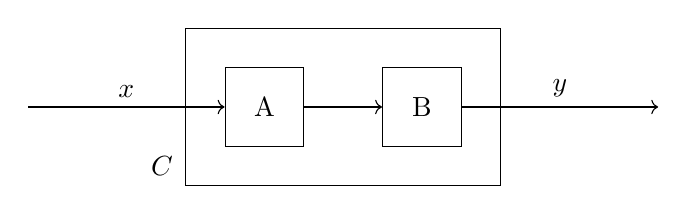
\begin{tikzpicture}
        % Define nodes for blocks A and B
        \node[draw, rectangle, minimum width=1cm, minimum height=1cm] (A) at (0,0) {A};
        \node[draw, rectangle, minimum width=1cm, minimum height=1cm] (B) at (2,0) {B};
        
        % Draw the outer rectangle
        \draw (-1, 1) rectangle (3, -1);
        
        % Draw arrows and labels
        \draw[->] (-3, 0) -- (A.west) node[midway,above] {$x$};
        \draw[->] (A.east) -- (B.west);
        \draw[->] (B.east) -- (5, 0) node[midway,above] {$y$};
        
        % Label C 
        \node at (-1.3, -0.5) [below] {$C$};
    \end{tikzpicture}
\end{Described}
}
Let $c$ denote the impulse response of the cascade interconnection.

\begin{enumerate}[(i)]
\item Express $c$ in terms of $a$ and $b$.
    
\ans{

        The impulse response \(c\) of the cascade interconnection is given by 
        \begin{equation*}
            c[n] = (a * b)[n] = \sum_{k=-\infty}^{\infty} a[k]\,b[n-k]
        \end{equation*}
         Substituting \(n = 0\):
        \begin{equation*}
            c_0 = a_0 b_0
        \end{equation*}
        \(n = 1\):
        \begin{equation*}
            c_1 = a_0 b_1 + a_1 b_0 
        \end{equation*}
        \(n = 2\):
        \begin{equation*}
            c_2 = a_0 b_2 + a_1 b_1 + a_2 b_0
        \end{equation*}
        And so on...
    
        Thus, we can write:
        \begin{equation*}
            c_n = \sum_{k=\max(0,n-M)}^{\min(n, N)} a_k b_{n-k}
        \end{equation*}
        \null\hfill for \(n = 0, 1, \ldots, N + M\)
        
        where we found the bounds of summation from the two conditions that ensure we are indexing \(a[n]\) and \(b[n]\) without exceeding the bounds of their signal.
        $$ 0 \leq k \leq N \Longrightarrow k \leq N \quad \text{and} \quad k \geq 0 $$
        $$ 0 \leq n - k \leq M \Longrightarrow k \leq n \quad \text{and} \quad k \geq n - M $$
        and so
        $$ k \leq \min(n, N) \quad \text{and} \quad k \geq \max(0, n-M) $$

        Lastly, 
         \begin{equation*}
            c[n] = c_0\delta[n] + c_1 \delta[n - 1] + ... + c_{N + M} \delta[n - ( N + M)]
        \end{equation*}
        
    }

\item Consider two polynomials $A(z)$ and $B(z)$ described as follows:
    $$
    A(z) = a_0 +a_1 z + \cdots + a_N z^N \quad \quad \quad B(z) = b_0 +b_1 z + \cdots + b_M z^M \, ,
    $$
    where $M$ and $N$ and positive integers.
    Let $C(z)=A(z)\, B(z)$, where $$ C(z) = c_0 +c_1 z + \cdots + c_{N+M} z^{N+M}.$$  Show that multiplying polynomials is tantamount to convolving their coefficients; in particular, explain how $c_n=(a*b)_n=\displaystyle\sum_m a_m b_{n-m}$, where $n={0,1,\ldots, N+M}$.
    
    \ans{
    \begin{equation*}
        C(z) = (a_0 +a_1 z + \cdots + a_N z^N) (b_0 +b_1 z + \cdots + b_M z^M)
    \end{equation*}
    \begin{equation*}
        C(z) = a_0 b_0 + (a_0 b_1 + a_1 b_0) z + (a_0 b_2 + a_1 b_1 + a_2 b_0) z^2 + ...
    \end{equation*}
    As you can see, each coefficient of \(z^n\) is the sum of all products of \(a_i\) and \(b_j\) where \(i + j = n\):
    \begin{equation*}
        c_n =  \sum_{m=\max(0,n-M)}^{\min(n, N)} a_m b_{n-m}
    \end{equation*}
    \null\hfill for \(n = 0, 1, 2, ..., N + M\)

    Just like the definition of convolution!
    }

\end{enumerate}
\end{enumerate}
  \newpage
  \qns{Frequency Response from a DAG Block Diagram [Adapted from EE 120]}
% Adapted by Ken Zheng for EECS 16A Fall 2025 Discussion

    Consider a DT LTI system with input $x[n]$ and output $y[n]$ that is implemented by the following block diagram:
    \begin{figure}[h!]
      \centering
      \begin{Described}{Block diagram: input x of n enters a summing junction whose output is y of n. That output is tapped, passed through a delay block D and then a gain of minus 0.5, and fed back into the summing junction.}
\begin{circuitikz}
          \node (x) at (0, 0) {$x[n]$};
          \node[circle, draw] (sum) at (2, 0) {$+$};
          % FIXME: find a better way to draw the triangle
          % \node[triangleblock, shape border rotate=90, inner sep=-1mm] (gain) at (3, -1.5) {$-0.5$};
          % \node at (3, -1.5) {$-0.5$};
          \node[draw, inner sep=5pt] (delay) at (6, -1.5) {$D$};
          \node (y) at (9, 0) {$y[n]$};
          \draw[->] (x.east) -- (sum.west);
          \draw[->] (sum.east) -- (y.west);
          \draw[->] (7.5, 0) -- (7.5, -1.5) -- (delay.east);
          % \draw[-, thick] (delay.west) -- (gain.east);
          % \draw[->, thick] (gain.west) -- (2, -1.5) -- (sum.south);
          \draw[->] (delay.west) to [amp, t=$-0.5$, blocks/scale=1.5] (2, -1.5) to (sum.south);
      \end{circuitikz}
\end{Described}
  \end{figure}
\begin{enumerate}
        \item Find the LCCDE that describes this system. 
        
        \ans{
            The difference equation describing this system is
              \begin{equation*}
                y[n] = x[n] - 0.5y[n-1]
              \end{equation*}
        }

        \item Find the frequency response $H(\omega)$ of this system. 
            
        \ans{
            Using the eigenfunction property by setting $x[n] = e^{i\omega n}$ and $y[n] = H(\omega) e^{i\omega n}$,
            \begin{align*}
            H(\omega) e^{i\omega n} &= e^{i\omega n} - 0.5 H(\omega) e^{i\omega (n-1)} \\
            &= e^{i\omega n} - 0.5 H(\omega) e^{-i\omega}e^{i\omega n} \\
            \left(1 + 0.5 e^{-i\omega}\right) e^{i\omega n} H(\omega) &= e^{i\omega n} \\
            H(\omega) &= \frac{e^{i\omega n}}{\left(1 + 0.5 e^{-i\omega}\right)e^{i\omega n}} \\
                &= \frac{1}{1 + 0.5 e^{-i\omega}}
            \end{align*} 
        } 

        \vspace{4cm}

        \item Is this a high pass or low pass filter?
        
        \ans{
            We can think about this in two ways:
            
            \textbf{1. Geometric Approach:}

            Recall from part (b) that the frequency response can be written as:
            \[
            H(\omega) = \frac{1}{1 + 0.5 e^{-i\omega}} = \frac{e^{i\omega}}{e^{i\omega} - (-0.5)}
            \]
            The magnitude is therefore:
            \[
            |H(\omega)| = \frac{1}{|e^{i\omega} - (-0.5)|}
            \]
            This represents the reciprocal of the distance from the point $e^{i\omega}$ on the unit circle to the point located at $-0.5$ on the real axis:

            \begin{center}
            \begin{Described}{Complex plane with real and imaginary axes and the unit circle centred at the origin. A point is marked at minus 0.5 on the real axis, with an arrow from it to the point e to the i omega on the circle.}
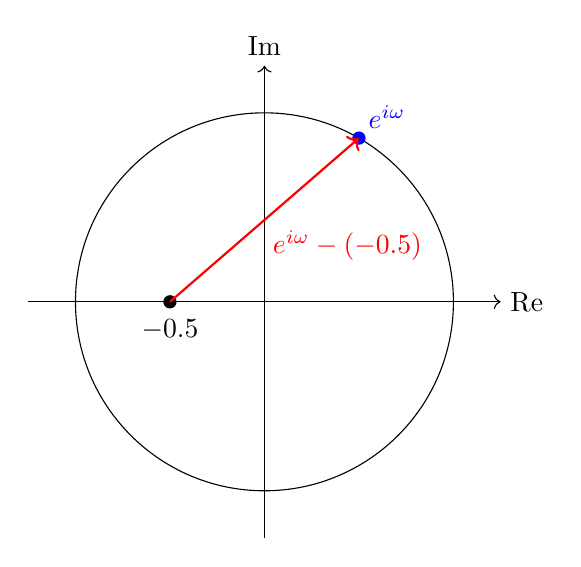
\begin{tikzpicture}[scale=1.2]
                % Axes
                \draw[->] (-2.5,0) -- (2.5,0) node[right] {$\operatorname{Re}$};
                \draw[->] (0,-2.5) -- (0,2.5) node[above] {$\operatorname{Im}$};

                % Unit circle
                \draw (0,0) circle (2);

                % Pole at -0.5
                \fill[black] (-1,0) circle (2pt) node[below left] {};
                \node[black] at (-1,-0.3) {$-0.5$};

                % Point on unit circle at angle ω
                \coordinate (P) at (60:2);
                \fill[blue] (P) circle (2pt) node[above right] {$e^{i\omega}$};

                % Vector from pole to point on circle
                % \draw[->, thick, red] (-1,0) -- (P);
                \draw[->, thick, red] (-1,0) -- (P) node[midway, below] {$\qquad\qquad\qquad e^{i \omega} - (-0.5)$};  % Label added here


                % Labels
                \node at (1.8,1.8) {};
            \end{tikzpicture}
\end{Described}
            \end{center}

            Key observations:
            \begin{itemize}
                \item When $\omega = 0$, $e^{i\omega} = 1$. The distance from $1$ to $-0.5$ is $1.5$, so $|H(0)| = 1/1.5 \approx 0.667$.
                \item When $\omega = \pi$, $e^{i\omega} = -1$. The distance from $-1$ to $-0.5$ is $0.5$, so $|H(\pi)| = 1/0.5 = 2$.
                \item As $\omega$ moves from $0$ to $\pi$, the point $e^{i\omega}$ travels along the upper half of the unit circle from $(1,0)$ to $(-1,0)$. 
                The distance to the point at $-0.5$ decreases monotonically, so $|H(\omega)|$ increases. Thus, we have a high-pass filter!\\
            \end{itemize}

            
            \textbf{2. Algebraic Approach:}
            
            To determine the filter type, we simplify the magnitude of the frequency response first:

            \[
            |H(\omega)| = \frac{1}{\sqrt{(1 + 0.5\cos\omega)^2 + (0.5\sin\omega)^2}}
            \]


            Expanding \( (1 + 0.5\cos\omega)^2 \) and \( (0.5\sin\omega)^2 \):
            \[
            (1 + 0.5\cos\omega)^2 = 1^2 + 2(1)(0.5\cos\omega) + (0.5\cos\omega)^2 = 1 + \cos\omega + 0.25\cos^2\omega
            \]
            \[
            (0.5\sin\omega)^2 = 0.25\sin^2\omega
            \]


            Add the two results in the square root:
            \[
            (1 + 0.5\cos\omega)^2 + (0.5\sin\omega)^2 = \left[1 + \cos\omega + 0.25\cos^2\omega\right] + \left[0.25\sin^2\omega\right]
            \]
            \[
            = 1 + \cos\omega + 0.25\left(\cos^2\omega + \sin^2\omega\right)
            \]
            \[
            = 1 + \cos\omega + 0.25(1) = 1 + \cos\omega + 0.25 = 1.25 + \cos\omega
            \]


            Substitute back into \( |H(\omega)| \):
            \[
            |H(\omega)| = \frac{1}{\sqrt{1.25 + \cos\omega}}
            \]
                        
            Now we analyze the magnitude at key frequencies:
            
            Low frequency (\( \omega = 0 \)): 
                \[
                |H(0)| =  \frac{1}{\sqrt{1.25 + \cos0}} = \frac{1}{1.5} \approx 0.667 \quad (\text{attenuated})
                \]
            High frequency (\( \omega = \pi \)): 
                \[
                |H(\pi)| =  \frac{1}{\sqrt{1.25 + \cos\pi}} = 2 \quad (\text{passed})
                \]

            We can see that, again, the filter attenuates low frequencies and passes high frequencies, so it is a high-pass filter!\\

            Both geometrically and algebraically, we conclude this is a \textbf{high-pass filter}. Nice!
        }
\end{enumerate}

  \newpage
  \qns{Using PCA to Detect Fraudulent Transactions (Adapted from EECS 16B Spring 2023 Final)}\\
	PCA has many different uses when applied to real-world data. One potential application is making classification of data much easier.
	
	Suppose we are given some data, where each datapoint represents a transaction. Each one is labeled either normal or fraudulent. We will utilize PCA to develop a useful classifier.

	We plot the data in two dimensions, where each dimension is some unspecified feature that will aid us in classifying the points:

	\begin{figure}[H]
        \centering
        \begin{Described}{Scatter plot on x and y axes running about minus 4 to 4, with four transactions marked: circles at (-3, -1) and (0, -2), and diamonds at (2, 0) and (1, 3).}
\begin{tikzpicture}
            \node (origin) at (0, 0) {};
            \node (top) at ($(origin) + (0, 4)$) {};
            \node (bottom) at ($(origin) + (0, -4)$) {};
            \node (left) at ($(origin) + (-4, 0)$) {};
            \node (right) at ($(origin) + (4, 0)$) {};
            \draw [->] (bottom) -- (top);
            \draw [->] (left) -- (right);
    
            \node at (-3, -2.2) (leftendpoint) {};
            \node at (3, 2.2) (rightendpoint) {};
            %\node at ($(origin) + (0.8, 1.3)$) {$y=\alpha x$};
            \node at ($(origin) + (3.9, -0.3)$) {$x$};
            \node at ($(origin) + (0.3, 4.0)$) {$y$};
    
            %\draw[line width=0.75mm] (leftendpoint) -- (rightendpoint);
    
            \node[circle, fill=black!60!green, inner sep=1.5pt] at ($({-3/1.0}, {-1/1.0})$) (dp1) {};
            \node[circle, fill=black!60!green, inner sep=1.5pt] at ($({0/1.0}, {-2/1.0})$) (dp2) {};
            \node[diamond, fill=red, inner sep=1.5pt] at ($({1/1.0}, {3/1.0})$) (dp3) {};
			\node[diamond, fill=red, inner sep=1.5pt] at ($({2/1.0}, {0/1.0})$) (dp4) {};
    
            \node at ($({1/1.0}, 0.1)$) (dp1x) {};
            \node at ($(-0.1, {-2/1.0})$) (dp1y) {};
            \node at ($({1/1.0}, 0.3)$) {$1$};
            \node at ($(-0.3, {-2/1.0})$) {$-2$};
            %\draw[dotted] (dp1) -- (dp1x);
            %\draw[dotted] (dp1) -- (dp1y);
    
            \node at ($({2/1.0}, -0.1)$) (dp2x) {};
            \node at ($(-0.1, {3/1.0})$) (dp2y) {};
            \node at ($({2/1.0}, -0.3)$) {$2$};
            \node at ($(-0.3, {3/1.0})$) {$3$};
            %\draw[dotted] (dp2) -- (dp2x);
            %\draw[dotted] (dp2) -- (dp2y);
    
            \node at ($({-3/1.0}, 0.1)$) (dp3x) {};
            \node at ($(0.1, {-1/1.0})$) (dp3y) {};
            \node at ($({-3/1.0}, 0.3)$) {$-3$};
            \node at ($(-0.3, {-1/1.0 -0.3} )$) {$-1$};
            %\draw[dotted] (dp3) -- (dp3x);
            %\draw[dotted] (dp3) -- (dp3y);
    
    
            \node[inner sep=0pt] at ($(leftendpoint)!(dp1)!(rightendpoint)$) (pdp1) {};
            \node[inner sep=0pt] at ($(leftendpoint)!(dp2)!(rightendpoint)$) (pdp2) {};
            \node[inner sep=0pt] at ($(leftendpoint)!(dp3)!(rightendpoint)$) (pdp3) {};
    
            %\draw[red] (dp1) -- (pdp1);
            %\draw[red] (dp2) -- (pdp2);
            %\draw[red] (dp3) -- (pdp3);
        \end{tikzpicture}
\end{Described}
        \caption{Plot of Transactions in 2-D}
	\end{figure}

	Thus, we have a total of 4 transactions, $\bmqty{-3 \\ -1}$ and $\bmqty{0 \\ -2}$ are normal, while $\bmqty{2 \\ 0}$ and $\bmqty{1 \\ 3}$ are fraudulent.
	\begin{enumerate}
		%Part A:
		
		\qitem Suppose we now construct a data matrix, where the \textit{data points are columns}. 

			\begin{equation}
				X = \bmqty{-3 & 0 & 2 & 1 \\ -1 & -2 & 0 & 3}
			\end{equation}

			Using this data matrix, \textbf{calculate its first principal component $\vec{u}_1$}.

			\begin{hint}
			\begin{enumerate}

				\item You may also make use of the fact that $XX^T$ is given by:
				\begin{align}
					XX^{\top} &= \bmqty{-3 & 0 & 2 & 1 \\ -1 & -2 & 0 & 3}\bmqty{-3 & 0 & 2 & 1 \\ -1 & -2 & 0 & 3}^{\top} \\
						&= \bmqty{14 & 6 \\ 6 & 14}
				\end{align}
				\item You may also make use of the characteristic polynomial of $XX^T$:
				\begin{equation}
					\lambda^2 - 28\lambda + 160 = (\lambda - 20)(\lambda - 8) = 0
				\end{equation}
			\end{enumerate}
			\end{hint}
			
			\begin{hint} Remember that your principal component should be of unit norm. \end{hint}

		\ans{
			% From PCA, we know that our first principal component of a matrix with column data is the first column vector of $U$ in the SVD of $X$. Thus, we use the SVD method of calculation (find the eigenvector corresponding to the largest eigenvalue of $XX^{\top}$ and normalize to yield $\vec{u}_1$).

			% \begin{align}
			% 	XX^{\top} &= \bmqty{-3 & 0 & 2 & 1 \\ -1 & -2 & 0 & 3}\bmqty{-3 & 0 & 2 & 1 \\ -1 & -2 & 0 & 3}^{\top} \\
			% 		 &= \bmqty{14 & 6 \\ 6 & 14}
			% \end{align}

			% From setting $\mathrm{det}(XX^{\top} - \lambda I) = 0$, we should find our characteristic polynomial to be 
			
			% \begin{equation}
			% 	\lambda^2 - 28\lambda + 160 = 0
			% \end{equation}

			Our eigenvalues are $\lambda_1 = 20$ and $\lambda_2 = 8$. Thus, the eigenvector corresponding to our largest eigenvalue $\lambda_1 = 20$ is $\vec{v}_1 = \bmqty{1 \\ 1}$ from inspection.
			
			Thus, our principal component vector is given as the normalized eigenvector: i.e. $\vec{u}_1 = \bmqty{\frac{1}{\sqrt{2}} \\ \frac{1}{\sqrt{2}}}$.
        }

		%Part B:
		
		\qitem	It's difficult to come up with a useful classifier in two dimensions. Let's use PCA dimensionality reduction to help.
			
			Using your answer in part (a), \textbf{project your two-dimensional data points onto one dimension. Express your answer as the vector $\vec{z} \in \mathbb{R}^{1 \times 4}$.}

		\ans{
			To project our 2-d data into 1-d, we project our data matrix onto the first principal component as follows:
			
			\begin{equation}
				\vec{z} = \vec{u}_1^{\top}X = \bmqty{\frac{1}{\sqrt{2}} \\ \frac{1}{\sqrt{2}}} \bmqty{-3 & 0 & 2 & 1 \\ -1 & -2 & 0 & 3} = \bmqty{-\frac{4}{\sqrt{2}} & -\frac{2}{\sqrt{2}} & \frac{2}{\sqrt{2}} & \frac{4}{\sqrt{2}}}
			\end{equation}
		}
		
		%Part C:
		
		\qitem	Now, plot each of these points, on the line below. Indicate the value and label (normal as circle and fraudulent as diamond) for each point.
			
			\textit{Note: your plot doesn't have to be to scale.}

			\begin{figure}[H]
				\centering
				\begin{Described}{Blank horizontal number line labelled z, with only the origin marked 0 and no points plotted.}
\begin{tikzpicture}
					\node (origin) at (0, 0) {|};
            		%\node (top) at ($(origin) + (0, 4)$) {};
            		%\node (bottom) at ($(origin) + (0, -4)$) {};
            		\node (left) at ($(origin) + (-4, 0)$) {};
            		\node (right) at ($(origin) + (4, 0)$) {};
					\node at ($(origin) + (3.9, -0.3)$) {$z$};
					\node at ($(origin) + (0, -0.3)$) {0};
            		%\draw [->] (bottom) -- (top);
            		\draw [<->] (left) -- (right);

				\end{tikzpicture}
\end{Described}
				\caption{Plot of Transactions in 1-D}
			\end{figure}

		\ans{
			\begin{figure}[H]
				\centering
				\begin{Described}{Number line labelled z with the origin marked 0 and four points: circles at minus four over root two and minus two over root two, diamonds at two over root two and four over root two.}
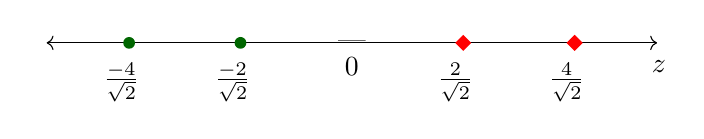
\begin{tikzpicture}
					\node (origin) at (0, 0) {|};
            		%\node (top) at ($(origin) + (0, 4)$) {};
            		%\node (bottom) at ($(origin) + (0, -4)$) {};
            		\node (left) at ($(origin) + (-4, 0)$) {};
            		\node (right) at ($(origin) + (4, 0)$) {};
					\node at ($(origin) + (3.9, -0.3)$) {$z$};
					\node at ($(origin) + (0, -0.3)$) {0};
            		%\draw [->] (bottom) -- (top);
            		\draw [<->] (left) -- (right);

					\node[circle, fill=black!60!green, inner sep=1.5pt] at ($(origin) + (-4/1.414, 0)$) (dp1) {};
					\node at ($(origin) + (-4/1.414 -0.1, -0.5)$) {$\frac{-4}{\sqrt{2}}$};
					\node[circle, fill=black!60!green, inner sep=1.5pt] at ($(origin) + (-2/1.414, 0)$) (dp1) {};
					\node at ($(origin) + (-2/1.414 -0.1, -0.5)$) {$\frac{-2}{\sqrt{2}}$};
					\node[diamond, fill=red, inner sep=1.5pt] at ($(origin) + (2/1.414, 0)$) (dp1) {};
					\node at ($(origin) + (2/1.414 -0.1, -0.5)$) {$\frac{2}{\sqrt{2}}$};
					\node[diamond, fill=red, inner sep=1.5pt] at ($(origin) + (4/1.414, 0)$) (dp1) {};
					\node at ($(origin) + (4/1.414 -0.1, -0.5)$) {$\frac{4}{\sqrt{2}}$};
				\end{tikzpicture}
\end{Described}
				\caption{Plot of Transactions in 1-D}
			\end{figure}
		}

		%Part D:
		
		\qitem	Suppose you are given some transaction datapoint, $\vec{x}_i$ and you project it to be one-dimensional, i.e. $z_i$. \textbf{Based on your plot from part (c), come up with an inequality in terms of $z_i$ to identify if that transaction is fraudulent.}
			
			\textit{Note: There can be more than one answer, but please only give one.}

		\ans{
			$\vec{z}_i > 0$ is a possible answer. In fact any answer in between $\vec{z}_i \geq -\frac{2}{\sqrt{2}}$ and $\vec{z}_i \geq \frac{2}{\sqrt{2}}$ is valid.
		}

		%Part E:
		
		\qitem	It can often be informative to compare our original data with its PCA reconstructions. \textbf{Using PCA, reconstruct $\vec{z}$ back into 2-D as the matrix $\wt{X} \in \mathbb{R}^{2 \times 4}$.}

		\ans{
			Using the reconstruction principle of PCA, we lift the 1D data back into 2 dimensions by doing the following:
			\begin{equation}
				\wt{X} = \vec{u}_1\vec{u}_1^{\top}X = \bmqty{-2 & -1 & 1 & 2 \\ -2 & -1 & 1 & 2}
			\end{equation}
		}

		%Part F:
		
		\qitem	Finally, we visualize our PCA reconstruction. \textbf{On the graph below, draw your first principal component direction (extend it as a solid line in both directions). Draw your reconstructioned points from $\wt{X}$, with dotted lines connecting them with the corresponding point in $X$. } You may draw on the plot on the next page.

			\begin{figure}[H]
				\centering
				\begin{Described}{Scatter plot on x and y axes running about minus 4 to 4, with four transactions marked: circles at (-3, -1) and (0, -2), and diamonds at (2, 0) and (1, 3).}
\begin{tikzpicture}
					\node (origin) at (0, 0) {};
					\node (top) at ($(origin) + (0, 4)$) {};
					\node (bottom) at ($(origin) + (0, -4)$) {};
					\node (left) at ($(origin) + (-4, 0)$) {};
					\node (right) at ($(origin) + (4, 0)$) {};
					\draw [->] (bottom) -- (top);
					\draw [->] (left) -- (right);
			
					\node at (-3, -2.2) (leftendpoint) {};
					\node at (3, 2.2) (rightendpoint) {};
					%\node at ($(origin) + (0.8, 1.3)$) {$y=\alpha x$};
					\node at ($(origin) + (3.9, -0.3)$) {$x$};
					\node at ($(origin) + (0.3, 4.0)$) {$y$};
			
					%\draw[line width=0.75mm] (leftendpoint) -- (rightendpoint);
			
					\node[circle, fill=black!60!green, inner sep=1.5pt] at ($({-3/1.0}, {-1/1.0})$) (dp1) {};
					\node[circle, fill=black!60!green, inner sep=1.5pt] at ($({0/1.0}, {-2/1.0})$) (dp2) {};
					\node[diamond, fill=red, inner sep=1.5pt] at ($({1/1.0}, {3/1.0})$) (dp3) {};
					\node[diamond, fill=red, inner sep=1.5pt] at ($({2/1.0}, {0/1.0})$) (dp4) {};
			
					\node at ($({1/1.0}, 0.1)$) (dp1x) {};
					\node at ($(-0.1, {-2/1.0})$) (dp1y) {};
					\node at ($({1/1.0}, 0.3)$) {$1$};
					\node at ($(-0.3, {-2/1.0})$) {$-2$};
					%\draw[dotted] (dp1) -- (dp1x);
					%\draw[dotted] (dp1) -- (dp1y);
			
					\node at ($({2/1.0}, -0.1)$) (dp2x) {};
					\node at ($(-0.1, {3/1.0})$) (dp2y) {};
					\node at ($({2/1.0}, -0.3)$) {$2$};
					\node at ($(-0.3, {3/1.0})$) {$3$};
					%\draw[dotted] (dp2) -- (dp2x);
					%\draw[dotted] (dp2) -- (dp2y);
			
					\node at ($({-3/1.0}, 0.1)$) (dp3x) {};
					\node at ($(0.1, {-1/1.0})$) (dp3y) {};
					\node at ($({-3/1.0}, 0.3)$) {$-3$};
					\node at ($(-0.3, {-1/1.0 -0.3} )$) {$-1$};
					%\draw[dotted] (dp3) -- (dp3x);
					%\draw[dotted] (dp3) -- (dp3y);
			
			
					\node[inner sep=0pt] at ($(leftendpoint)!(dp1)!(rightendpoint)$) (pdp1) {};
					\node[inner sep=0pt] at ($(leftendpoint)!(dp2)!(rightendpoint)$) (pdp2) {};
					\node[inner sep=0pt] at ($(leftendpoint)!(dp3)!(rightendpoint)$) (pdp3) {};
			
					%\draw[red] (dp1) -- (pdp1);
					%\draw[red] (dp2) -- (pdp2);
					%\draw[red] (dp3) -- (pdp3);
				\end{tikzpicture}
\end{Described}
				\caption{Plot of Transactions in 2-D}
			\end{figure}

		\ans{

			Using the answer from part (d), students should end up with the following graph:
			\begin{figure}[H]
				\centering
				\begin{Described}{The same four transactions, with a solid line through the origin along y = x and reconstructed points on it at (-2, -2), (-1, -1), (1, 1) and (2, 2), each joined to its original point by a dotted line.}
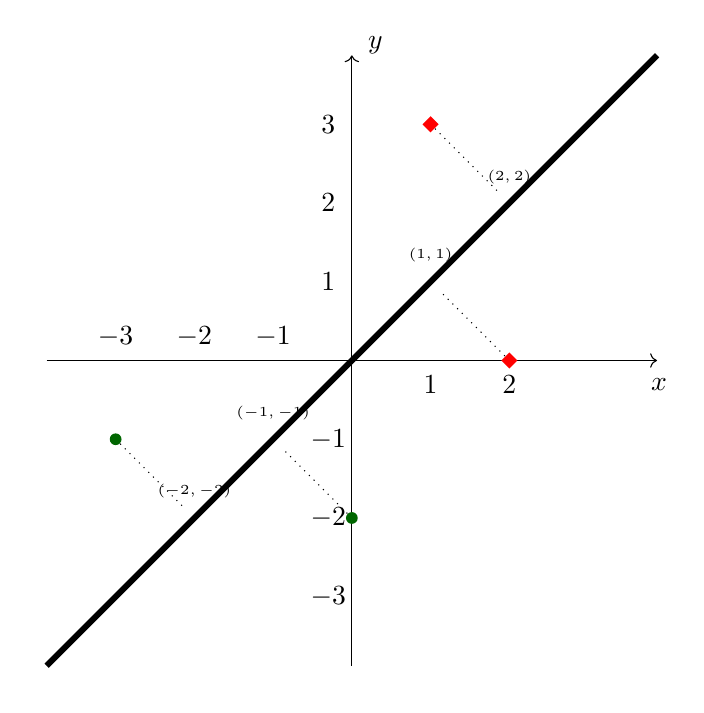
\begin{tikzpicture}
					\node (origin) at (0, 0) {};
					\node (top) at ($(origin) + (0, 4)$) {};
					\node (bottom) at ($(origin) + (0, -4)$) {};
					\node (left) at ($(origin) + (-4, 0)$) {};
					\node (right) at ($(origin) + (4, 0)$) {};
					\draw [->] (bottom) -- (top);
					\draw [->] (left) -- (right);
			
					\node at (-4, -4) (leftendpoint) {};
					\node at (4, 4) (rightendpoint) {};
					%\node at ($(origin) + (0.8, 1.3)$) {$y=\alpha x$};
					\node at ($(origin) + (3.9, -0.3)$) {$x$};
					\node at ($(origin) + (0.3, 4.0)$) {$y$};
			
					\draw[line width=0.75mm] (leftendpoint) -- (rightendpoint);
			
					\node[circle, fill=black!60!green, inner sep=1.5pt] at ($({-3/1.0}, {-1/1.0})$) (dp1) {};
					\node[circle, fill=black!60!green, inner sep=1.5pt] at ($({0/1.0}, {-2/1.0})$) (dp2) {};
					\node[diamond, fill=red, inner sep=1.5pt] at ($({2/1.0}, {0/1.0})$) (dp3) {};
					\node[diamond, fill=red, inner sep=1.5pt] at ($({1/1.0}, {3/1.0})$) (dp4) {};
					

					\node[label= {\tiny $\left( -2, -2\right)$}] at (-2, -2) (r1) {};
					\node[label= {\tiny $\left( -1, -1\right)$}] at (-1, -1) (r2) {};
					\node[label= {\tiny $\left( 1, 1\right)$}] at (1, 1) (r3) {};
					\node[label= {\tiny $\left( 2, 2\right)$}] at (2, 2) (r4) {};

					\draw[dotted] (dp1) -- (r1);
					\draw[dotted] (dp2) -- (r2);
					\draw[dotted] (dp3) -- (r3);
					\draw[dotted] (dp4) -- (r4);
			
					\node at ($({1/1.0}, 0.1)$) (dp1x) {};
					\node at ($(-0.1, {-2/1.0})$) (dp1y) {};
					\node at ($({1/1.0}, -0.3)$) {$1$};
					\node at ($(-0.3, {-2/1.0})$) {$-2$};
					%\draw[dotted] (dp1) -- (dp1x);
					%\draw[dotted] (dp1) -- (dp1y);
			
					\node at ($({2/1.0}, -0.1)$) (dp2x) {};
					\node at ($(-0.1, {3/1.0})$) (dp2y) {};
					\node at ($({2/1.0}, -0.3)$) {$2$};
					\node at ($(-0.3, {1/1.0})$) {$1$};
					\node at ($(-0.3, {2/1.0})$) {$2$};
					\node at ($(-0.3, {3/1.0})$) {$3$};
					%\draw[dotted] (dp2) -- (dp2x);
					%\draw[dotted] (dp2) -- (dp2y);
			
					\node at ($({-3/1.0}, 0.1)$) (dp3x) {};
					\node at ($(0.1, {-1/1.0})$) (dp3y) {};
					\node at ($({-3/1.0}, 0.3)$) {$-3$};
					\node at ($({-2/1.0}, 0.3)$) {$-2$};
					\node at ($({-1/1.0}, 0.3)$) {$-1$};
					\node at ($(-0.3, {-3/1.0} )$) {$-3$};
					\node at ($(-0.3, {-1/1.0} )$) {$-1$};
					%\draw[dotted] (dp3) -- (dp3x);
					%\draw[dotted] (dp3) -- (dp3y);
			
			
					\node[inner sep=0pt] at ($(leftendpoint)!(dp1)!(rightendpoint)$) (pdp1) {};
					\node[inner sep=0pt] at ($(leftendpoint)!(dp2)!(rightendpoint)$) (pdp2) {};
					\node[inner sep=0pt] at ($(leftendpoint)!(dp3)!(rightendpoint)$) (pdp3) {};
			
					%\draw[red] (dp1) -- (pdp1);
					%\draw[red] (dp2) -- (pdp2);
					%\draw[red] (dp3) -- (pdp3);
				\end{tikzpicture}
\end{Described}
				\caption{Plot of Transactions in 2-D}
			\end{figure}
		}


\end{enumerate}

  \newpage
  \qns{Diode System ID (Adapted from EECS 16B Fall 2023 Final)}

    \textbf{Note: This problem does not require knowledge of circuits or diodes.}
    
    Suppose that we want to characterize a diode $D_1$ with parasitic resistance $R_p$, represented by the following model:
    \begin{figure}[H]
        \begin{center}
            \begin{Described}{Voltage source V sub B drives from ground up to the top node, where diode D1 carries current I D to the right with voltage V D across it, in series with resistor R sub p returning to ground.}
\begin{circuitikz}
                \draw (0, 2) to [V, l_=$V_B$] (0, 0) node[ground]{}
                (0, 2) to [Do, l=$D_1$, i=$I_D$, v=$V_D$] (3, 2) to [R, l=$R_p$] (5, 2) node[ground]{}
                ;
            \end{circuitikz}
\end{Described}
        \end{center}
    \end{figure}
    The current through the diode (forward-biased) is modeled as
    \begin{equation}
        I_D = I_0\e^{\frac{V_D}{V_T}}
    \end{equation}
    where $V_D$ is the voltage across the diode (as shown in the diagram), $I_0$ is a parameter associated with the diode, and $V_T$ is the thermal voltage, a temperature dependent variable.
    
    With some analysis, the system equation can be simplified to:
    \begin{equation}
        I_D = I_0 \e^{\frac{V_B - I_D R_p}{V_T}}
    \end{equation}
    To collect data, we will vary the temperature to vary $V_T$ and measure the current $I_D$ through the diode.
    
        \begin{enumerate}

            \qitem    Use the provided system equation to show that
                \begin{equation}
                    I_D R_p - V_T \ln(I_0) = V_B - V_T \ln(I_D)
                \end{equation}
                    is a valid equation to represent the system.
                \begin{hint}
                    Use the logarithm identity $\ln(\frac{a}{b}) = \ln(a) - \ln(b)$.
                \end{hint}
            
    
            \ans{
                \begin{align}
                    I_D &= I_0 \e^{\frac{V_B - I_D R_p}{V_T}} \\
                    V_T\ln(\frac{I_D}{I_0}) &= V_B - I_D R_p \\
                    V_T\ln(I_D) - V_T\ln(I_0) &= V_B - I_D R_p \\
                    I_D R_p - V_T \ln(I_0) &= V_B - V_T \ln(I_D)
                \end{align}
            }
    
            % \begin{problempart}{4}{System ID}{0}{0}
            %     Suppose we use $V_B = 1 \mathrm{V}$ and collect the following data points:
            %     \begin{itemize}
            %         \item For $V_T = 0.025 \mathrm{V}$, $I_D = 0.0185 \mathrm{A}$.
            %         \item For $V_T = 0.05 \mathrm{V}$, $I_D = 0.0172 \mathrm{A}$.
            %         \item For $V_T = 0.0125 \mathrm{V}$, $I_D = 0.0193 \mathrm{A}$.
            %     \end{itemize}
            %     \textbf{Find the matrix $D$ and vector $\vec{s}$ to set up a least-squares problem $D\vec{p} \approx \vec{s}$ where $\vec{p} = \begin{bmatrix} \ln(I_0) \\ R_p \end{bmatrix}$.}
    
            %     You do not have to simplify the elements $D$ and $\vec{s}$, but the elements should be numerical values, not in terms of variables.
            % \end{problempart}
    
            % \begin{solution}{4in}
            %     Each data point can be used with the provided system equation from the first part to create a system of linear equations with the unknowns being $\ln(I_0)$ and $R_p$ (remember that the problem provides that $V_B = 1 \mathrm{V}$):
            %     \begin{itemize}
            %         \item $-0.025\ln(I_0) + 0.0185R_p = 1 - 0.025\ln(0.0185)$
            %         \item $-0.05\ln(I_0) + 0.0172R_p = 1 - 0.05\ln(0.0172)$
            %         \item $-0.0125\ln(I_0) + 0.0193R_p = 1 - 0.0125\ln(0.0193)$
            %     \end{itemize}
            %     The matrix form of this system is:
            %     \begin{equation}
            %         \begin{bmatrix} -0.025 & 0.0185 \\ -0.05 & 0.0172 \\ -0.0125 & 0.0193 \end{bmatrix} \begin{bmatrix} \ln(I_0) \\ R_p \end{bmatrix} = \begin{bmatrix} 1 - 0.025\ln(0.0185) \\ 1 - 0.05\ln(0.0172) \\ 1 - 0.0125\ln(0.0193) \end{bmatrix}
            %     \end{equation}
            %     Thus, for the least-squares problem, $D = \begin{bmatrix} -0.025 & 0.0185 \\ -0.05 & 0.0172 \\ -0.0125 & 0.0193 \end{bmatrix}$ and $\vec{s} = \begin{bmatrix} 1 - 0.025\ln(0.0185) \\ 1 - 0.05\ln(0.0172) \\ 1 - 0.0125\ln(0.0193) \end{bmatrix}$
            % \end{solution}
    
            \vspace{5cm}
            
            \qitem    Suppose we use $V_B = v_B$ and collect the following data points:
                \begin{itemize}
                    \item For $V_T = v_{T1}$, $I_D = i_{D1}$.
                    \item For $V_T = v_{T2}$, $I_D = i_{D2}$.
                    \item For $V_T = v_{T3}$, $I_D = i_{D3}$.
                \end{itemize}
                Find the matrix $\textbf{A}$ and vector $\vec{x}$ to set up a least-squares problem $\textbf{A} \vec{x} \approx \vec{b}$ where $\vec{x} = \begin{bmatrix} \ln(I_0) \\ R_p \end{bmatrix}$
    
            \ans{
                Each data point can be used with the provided system equation from the first part to create a system of linear equations with the unknowns being $\ln(I_0)$ and $R_p$ (remember that the problem provides that $V_B = v_B$):
                \begin{itemize}
                    \item $-v_{T1}\ln(I_0) + i_{D1}R_p = v_B - v_{T1}\ln(i_{D1})$
                    \item $-v_{T2}\ln(I_0) + i_{D2}R_p = v_B - v_{T2}\ln(i_{D2})$
                    \item $-v_{T3}\ln(I_0) + i_{D3}R_p = v_B - v_{T3}\ln(i_{D3})$
                \end{itemize}
                The matrix form of this system is:
                \begin{equation}
                    \begin{bmatrix} -v_{T1} & i_{D1} \\ -v_{T2} & i_{D2} \\ -v_{T3} & i_{D3} \end{bmatrix} \begin{bmatrix} \ln(I_0) \\ R_p \end{bmatrix} = \begin{bmatrix} v_B - v_{T1}\ln(i_{D1}) \\ v_B - v_{T2}\ln(i_{D2}) \\ v_B - v_{T3}\ln(i_{D3}) \end{bmatrix}
                \end{equation}
                Thus, for the least-squares problem, $\textbf{A} = \begin{bmatrix} -v_{T1} & i_{D1} \\ -v_{T2} & i_{D2} \\ -v_{T3} & i_{D3} \end{bmatrix}$ and $\vec{b} = \begin{bmatrix} v_B - v_{T1}\ln(i_{D1}) \\ v_B - v_{T2}\ln(i_{D2}) \\ v_B - v_{T3}\ln(i_{D3}) \end{bmatrix}$
            }
            
            \vspace{5cm}
            
            \qitem    Explain how you would use the least-squares system from the previous part to find model parameters $I_0$ and $R_p$. You do not need to use actual values for this part; you explanation can just use $\textbf{A}$ and $\vec{b}$ as known variables to show what calculations you would do to find $I_0$ and $R_p$.
            
    
            \ans{
                We would first find the optimal parameter $\hat{\vec{x}}$ with the least squares formula:
                \begin{equation}
                    \hat{\vec{x}} = (\textbf{A}^\top \textbf{A})^{-1} \textbf{A}^{\top} \vec{b}
                \end{equation}
                The elements of $\hat{\vec{x}}$ represent optimal values for $\ln(I_0)$ and $R_p$ so we set the elements of $\hat{\vec{x}}$ equal to those parameters for our model:
                \begin{align}
                    \hat{x}_{v_B} = \ln(I_0) &\rightarrow I_0 = \e^{\hat{x}_1} \\
                    \hat{x}_2 = R_p &\rightarrow R_p = \hat{x}_2
                \end{align}
                Thus, we have found parameter values for $I_0$ and $R_p$ from the least-squares system.
            }
    
        \end{enumerate}

\end{qunlist}

\end{document}
"
%   pdflatex "\PassOptionsToClass{prob}{latexally-assignment}% Demonstration built from REAL EECS 16A questionBank material, not from
% invented figures. Four question files were copied verbatim out of the corpus
% into corpus/ below, and `latexally apply` wrapped each figure in Described
% with a hand-written description. Nothing else in them was touched.
%
%   corpus/questionBank/sec/13/q_polynomial_fir_convolution.tex   1 figure
%   corpus/questionBank/sec/13/q_freq_resp_dag_diagram.tex        2 figures
%   corpus/sp26/dis/13A/questions/q_pca.tex                       4 figures
%   corpus/sp26/dis/13A/questions/q_diode_ls.tex                  1 figure
%
% Build both variants from this ONE source; build.sh supplies the class option:
%   pdflatex "\PassOptionsToClass{sol}{latexally-assignment}% Demonstration built from REAL EECS 16A questionBank material, not from
% invented figures. Four question files were copied verbatim out of the corpus
% into corpus/ below, and `latexally apply` wrapped each figure in Described
% with a hand-written description. Nothing else in them was touched.
%
%   corpus/questionBank/sec/13/q_polynomial_fir_convolution.tex   1 figure
%   corpus/questionBank/sec/13/q_freq_resp_dag_diagram.tex        2 figures
%   corpus/sp26/dis/13A/questions/q_pca.tex                       4 figures
%   corpus/sp26/dis/13A/questions/q_diode_ls.tex                  1 figure
%
% Build both variants from this ONE source; build.sh supplies the class option:
%   pdflatex "\PassOptionsToClass{sol}{latexally-assignment}\input{demo-questionbank}"
%   pdflatex "\PassOptionsToClass{prob}{latexally-assignment}\input{demo-questionbank}"

\DocumentMetadata{
  lang       = en-US,
  pdfversion = 2.0,
  testphase  = {phase-III,math,table,graphic,firstaid},
}
\documentclass{latexally-assignment}

\usepackage{amsmath,amssymb}
\usepackage{float}
\usepackage{tikz}
\usetikzlibrary{calc,shapes.geometric,positioning}
\usepackage[american]{circuitikz}

% The corpus macros these four files use, reproduced from questionBank/ee16.sty
% and questionBank/sp26/sp26.sty so the demo does not need the whole course
% preamble chain. Same meanings, nothing more.
\providecommand{\bmqty}[1]{\begin{bmatrix}#1\end{bmatrix}}
\providecommand{\e}{\mathop{\mathrm{e}}\nolimits}
\providecommand{\wt}[1]{\widetilde{#1}}
\NewDocumentEnvironment{hint}{+b}{\itshape (HINT: #1)}{}

\setcoursenumber{EECS 16A}
\setcoursename{Designing Information Devices and Systems I}
\setsemester{Spring 2026}

\begin{document}

\def\title{Described figures from the question bank}
\maketitle

\vspace{0.5em}
Every figure below carries a description in the PDF structure tree. A screen
reader announces "graphic" and then that description; it never reaches the
drawing underneath. Hovering shows nothing --- \texttt{/Alt} is not a tooltip.

\begin{qunlist}

  \input{corpus/questionBank/sec/13/q_polynomial_fir_convolution.tex}
  \newpage
  \input{corpus/questionBank/sec/13/q_freq_resp_dag_diagram.tex}
  \newpage
  \input{corpus/sp26/dis/13A/questions/q_pca.tex}
  \newpage
  \input{corpus/sp26/dis/13A/questions/q_diode_ls.tex}

\end{qunlist}

\end{document}
"
%   pdflatex "\PassOptionsToClass{prob}{latexally-assignment}% Demonstration built from REAL EECS 16A questionBank material, not from
% invented figures. Four question files were copied verbatim out of the corpus
% into corpus/ below, and `latexally apply` wrapped each figure in Described
% with a hand-written description. Nothing else in them was touched.
%
%   corpus/questionBank/sec/13/q_polynomial_fir_convolution.tex   1 figure
%   corpus/questionBank/sec/13/q_freq_resp_dag_diagram.tex        2 figures
%   corpus/sp26/dis/13A/questions/q_pca.tex                       4 figures
%   corpus/sp26/dis/13A/questions/q_diode_ls.tex                  1 figure
%
% Build both variants from this ONE source; build.sh supplies the class option:
%   pdflatex "\PassOptionsToClass{sol}{latexally-assignment}\input{demo-questionbank}"
%   pdflatex "\PassOptionsToClass{prob}{latexally-assignment}\input{demo-questionbank}"

\DocumentMetadata{
  lang       = en-US,
  pdfversion = 2.0,
  testphase  = {phase-III,math,table,graphic,firstaid},
}
\documentclass{latexally-assignment}

\usepackage{amsmath,amssymb}
\usepackage{float}
\usepackage{tikz}
\usetikzlibrary{calc,shapes.geometric,positioning}
\usepackage[american]{circuitikz}

% The corpus macros these four files use, reproduced from questionBank/ee16.sty
% and questionBank/sp26/sp26.sty so the demo does not need the whole course
% preamble chain. Same meanings, nothing more.
\providecommand{\bmqty}[1]{\begin{bmatrix}#1\end{bmatrix}}
\providecommand{\e}{\mathop{\mathrm{e}}\nolimits}
\providecommand{\wt}[1]{\widetilde{#1}}
\NewDocumentEnvironment{hint}{+b}{\itshape (HINT: #1)}{}

\setcoursenumber{EECS 16A}
\setcoursename{Designing Information Devices and Systems I}
\setsemester{Spring 2026}

\begin{document}

\def\title{Described figures from the question bank}
\maketitle

\vspace{0.5em}
Every figure below carries a description in the PDF structure tree. A screen
reader announces "graphic" and then that description; it never reaches the
drawing underneath. Hovering shows nothing --- \texttt{/Alt} is not a tooltip.

\begin{qunlist}

  \input{corpus/questionBank/sec/13/q_polynomial_fir_convolution.tex}
  \newpage
  \input{corpus/questionBank/sec/13/q_freq_resp_dag_diagram.tex}
  \newpage
  \input{corpus/sp26/dis/13A/questions/q_pca.tex}
  \newpage
  \input{corpus/sp26/dis/13A/questions/q_diode_ls.tex}

\end{qunlist}

\end{document}
"

\DocumentMetadata{
  lang       = en-US,
  pdfversion = 2.0,
  testphase  = {phase-III,math,table,graphic,firstaid},
}
\documentclass{latexally-assignment}

\usepackage{amsmath,amssymb}
\usepackage{float}
\usepackage{tikz}
\usetikzlibrary{calc,shapes.geometric,positioning}
\usepackage[american]{circuitikz}

% The corpus macros these four files use, reproduced from questionBank/ee16.sty
% and questionBank/sp26/sp26.sty so the demo does not need the whole course
% preamble chain. Same meanings, nothing more.
\providecommand{\bmqty}[1]{\begin{bmatrix}#1\end{bmatrix}}
\providecommand{\e}{\mathop{\mathrm{e}}\nolimits}
\providecommand{\wt}[1]{\widetilde{#1}}
\NewDocumentEnvironment{hint}{+b}{\itshape (HINT: #1)}{}

\setcoursenumber{EECS 16A}
\setcoursename{Designing Information Devices and Systems I}
\setsemester{Spring 2026}

\begin{document}

\def\title{Described figures from the question bank}
\maketitle

\vspace{0.5em}
Every figure below carries a description in the PDF structure tree. A screen
reader announces "graphic" and then that description; it never reaches the
drawing underneath. Hovering shows nothing --- \texttt{/Alt} is not a tooltip.

\begin{qunlist}

  \qns{Polynomial Multiplication and Discrete-Time Convolution [Adapted from EE 120]}
% Adapted and extended by Ken Zheng for EECS 16A Fall 2025 Discussion

The impulse response of a real, discrete-time FIR filter $\mathsf{A}$ is described by  
$$a[n]=a_0 \delta[n]+a_1 \delta[n-1]+\cdots + a_N \delta[n-N], \quad \text{where } N\in \{1,2,3,\ldots\}.$$

\begin{enumerate}[(a)]
\item Show that the frequency response $A(\omega)$ of the filter is a polynomial, in terms of $e^{-i\omega}$, whose coefficients have a simple relationship with the impulse response values $a_0,\ldots,a_N$.

\ans{

    Substituting \(a[n]\) into the frequency response formula we see that:
    \begin{equation*}
        A(w) = \sum_{n=-\infty}^{\infty} a[n]e^{-iwn}
    \end{equation*}
    As $a[n] = 0$ outside the range of $n = 0$ to $n = N$ ,
    \begin{equation*}
        A(w) = a_0 e^{-iw\cdot 0} + a_1 e^{-iw\cdot 1} + \ldots + a_N e^{-iw\cdot N}
    \end{equation*}
    \begin{equation*}
        = a_0 + a_1 e^{-iw} + \ldots + a_N e^{-iwN}
    \end{equation*}
}
\item Suppose the filter $\mathsf{A}$ is placed in a cascade (series) interconnection with another discrete-time FIR filter $\mathsf{B}$ whose impulse response is described by  
$$b[n]=b_0 \delta[n]+b_1 \delta[n-1]+\cdots + b_M \delta[n-M],\quad \text{where } M\in \{1,2,3,\ldots\}.$$

The cascade structure, which we call $\mathsf{C}$, is shown in the figure below.
\vspace{4pt}

\centerline{
    \begin{Described}{Block diagram: input x enters block A, whose output feeds block B, and block B's output is y. An outer box enclosing both blocks is labelled C.}
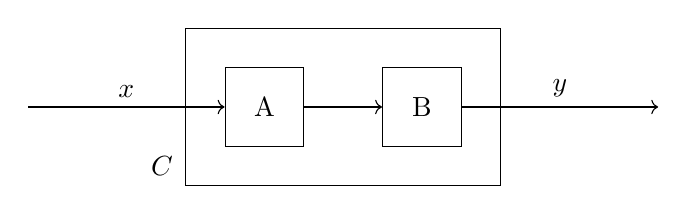
\begin{tikzpicture}
        % Define nodes for blocks A and B
        \node[draw, rectangle, minimum width=1cm, minimum height=1cm] (A) at (0,0) {A};
        \node[draw, rectangle, minimum width=1cm, minimum height=1cm] (B) at (2,0) {B};
        
        % Draw the outer rectangle
        \draw (-1, 1) rectangle (3, -1);
        
        % Draw arrows and labels
        \draw[->] (-3, 0) -- (A.west) node[midway,above] {$x$};
        \draw[->] (A.east) -- (B.west);
        \draw[->] (B.east) -- (5, 0) node[midway,above] {$y$};
        
        % Label C 
        \node at (-1.3, -0.5) [below] {$C$};
    \end{tikzpicture}
\end{Described}
}
Let $c$ denote the impulse response of the cascade interconnection.

\begin{enumerate}[(i)]
\item Express $c$ in terms of $a$ and $b$.
    
\ans{

        The impulse response \(c\) of the cascade interconnection is given by 
        \begin{equation*}
            c[n] = (a * b)[n] = \sum_{k=-\infty}^{\infty} a[k]\,b[n-k]
        \end{equation*}
         Substituting \(n = 0\):
        \begin{equation*}
            c_0 = a_0 b_0
        \end{equation*}
        \(n = 1\):
        \begin{equation*}
            c_1 = a_0 b_1 + a_1 b_0 
        \end{equation*}
        \(n = 2\):
        \begin{equation*}
            c_2 = a_0 b_2 + a_1 b_1 + a_2 b_0
        \end{equation*}
        And so on...
    
        Thus, we can write:
        \begin{equation*}
            c_n = \sum_{k=\max(0,n-M)}^{\min(n, N)} a_k b_{n-k}
        \end{equation*}
        \null\hfill for \(n = 0, 1, \ldots, N + M\)
        
        where we found the bounds of summation from the two conditions that ensure we are indexing \(a[n]\) and \(b[n]\) without exceeding the bounds of their signal.
        $$ 0 \leq k \leq N \Longrightarrow k \leq N \quad \text{and} \quad k \geq 0 $$
        $$ 0 \leq n - k \leq M \Longrightarrow k \leq n \quad \text{and} \quad k \geq n - M $$
        and so
        $$ k \leq \min(n, N) \quad \text{and} \quad k \geq \max(0, n-M) $$

        Lastly, 
         \begin{equation*}
            c[n] = c_0\delta[n] + c_1 \delta[n - 1] + ... + c_{N + M} \delta[n - ( N + M)]
        \end{equation*}
        
    }

\item Consider two polynomials $A(z)$ and $B(z)$ described as follows:
    $$
    A(z) = a_0 +a_1 z + \cdots + a_N z^N \quad \quad \quad B(z) = b_0 +b_1 z + \cdots + b_M z^M \, ,
    $$
    where $M$ and $N$ and positive integers.
    Let $C(z)=A(z)\, B(z)$, where $$ C(z) = c_0 +c_1 z + \cdots + c_{N+M} z^{N+M}.$$  Show that multiplying polynomials is tantamount to convolving their coefficients; in particular, explain how $c_n=(a*b)_n=\displaystyle\sum_m a_m b_{n-m}$, where $n={0,1,\ldots, N+M}$.
    
    \ans{
    \begin{equation*}
        C(z) = (a_0 +a_1 z + \cdots + a_N z^N) (b_0 +b_1 z + \cdots + b_M z^M)
    \end{equation*}
    \begin{equation*}
        C(z) = a_0 b_0 + (a_0 b_1 + a_1 b_0) z + (a_0 b_2 + a_1 b_1 + a_2 b_0) z^2 + ...
    \end{equation*}
    As you can see, each coefficient of \(z^n\) is the sum of all products of \(a_i\) and \(b_j\) where \(i + j = n\):
    \begin{equation*}
        c_n =  \sum_{m=\max(0,n-M)}^{\min(n, N)} a_m b_{n-m}
    \end{equation*}
    \null\hfill for \(n = 0, 1, 2, ..., N + M\)

    Just like the definition of convolution!
    }

\end{enumerate}
\end{enumerate}
  \newpage
  \qns{Frequency Response from a DAG Block Diagram [Adapted from EE 120]}
% Adapted by Ken Zheng for EECS 16A Fall 2025 Discussion

    Consider a DT LTI system with input $x[n]$ and output $y[n]$ that is implemented by the following block diagram:
    \begin{figure}[h!]
      \centering
      \begin{Described}{Block diagram: input x of n enters a summing junction whose output is y of n. That output is tapped, passed through a delay block D and then a gain of minus 0.5, and fed back into the summing junction.}
\begin{circuitikz}
          \node (x) at (0, 0) {$x[n]$};
          \node[circle, draw] (sum) at (2, 0) {$+$};
          % FIXME: find a better way to draw the triangle
          % \node[triangleblock, shape border rotate=90, inner sep=-1mm] (gain) at (3, -1.5) {$-0.5$};
          % \node at (3, -1.5) {$-0.5$};
          \node[draw, inner sep=5pt] (delay) at (6, -1.5) {$D$};
          \node (y) at (9, 0) {$y[n]$};
          \draw[->] (x.east) -- (sum.west);
          \draw[->] (sum.east) -- (y.west);
          \draw[->] (7.5, 0) -- (7.5, -1.5) -- (delay.east);
          % \draw[-, thick] (delay.west) -- (gain.east);
          % \draw[->, thick] (gain.west) -- (2, -1.5) -- (sum.south);
          \draw[->] (delay.west) to [amp, t=$-0.5$, blocks/scale=1.5] (2, -1.5) to (sum.south);
      \end{circuitikz}
\end{Described}
  \end{figure}
\begin{enumerate}
        \item Find the LCCDE that describes this system. 
        
        \ans{
            The difference equation describing this system is
              \begin{equation*}
                y[n] = x[n] - 0.5y[n-1]
              \end{equation*}
        }

        \item Find the frequency response $H(\omega)$ of this system. 
            
        \ans{
            Using the eigenfunction property by setting $x[n] = e^{i\omega n}$ and $y[n] = H(\omega) e^{i\omega n}$,
            \begin{align*}
            H(\omega) e^{i\omega n} &= e^{i\omega n} - 0.5 H(\omega) e^{i\omega (n-1)} \\
            &= e^{i\omega n} - 0.5 H(\omega) e^{-i\omega}e^{i\omega n} \\
            \left(1 + 0.5 e^{-i\omega}\right) e^{i\omega n} H(\omega) &= e^{i\omega n} \\
            H(\omega) &= \frac{e^{i\omega n}}{\left(1 + 0.5 e^{-i\omega}\right)e^{i\omega n}} \\
                &= \frac{1}{1 + 0.5 e^{-i\omega}}
            \end{align*} 
        } 

        \vspace{4cm}

        \item Is this a high pass or low pass filter?
        
        \ans{
            We can think about this in two ways:
            
            \textbf{1. Geometric Approach:}

            Recall from part (b) that the frequency response can be written as:
            \[
            H(\omega) = \frac{1}{1 + 0.5 e^{-i\omega}} = \frac{e^{i\omega}}{e^{i\omega} - (-0.5)}
            \]
            The magnitude is therefore:
            \[
            |H(\omega)| = \frac{1}{|e^{i\omega} - (-0.5)|}
            \]
            This represents the reciprocal of the distance from the point $e^{i\omega}$ on the unit circle to the point located at $-0.5$ on the real axis:

            \begin{center}
            \begin{Described}{Complex plane with real and imaginary axes and the unit circle centred at the origin. A point is marked at minus 0.5 on the real axis, with an arrow from it to the point e to the i omega on the circle.}
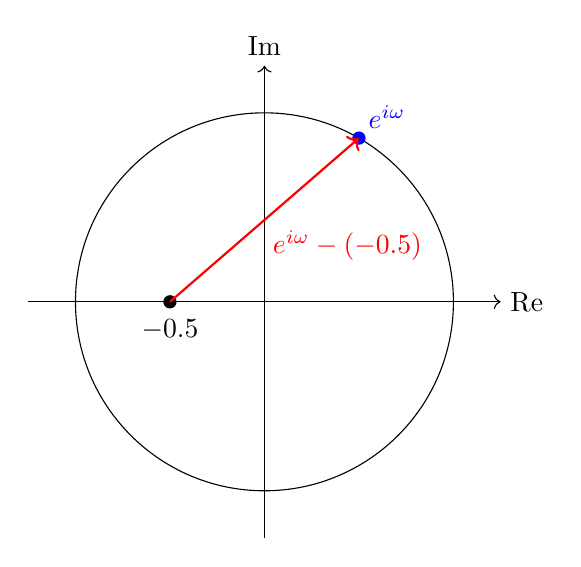
\begin{tikzpicture}[scale=1.2]
                % Axes
                \draw[->] (-2.5,0) -- (2.5,0) node[right] {$\operatorname{Re}$};
                \draw[->] (0,-2.5) -- (0,2.5) node[above] {$\operatorname{Im}$};

                % Unit circle
                \draw (0,0) circle (2);

                % Pole at -0.5
                \fill[black] (-1,0) circle (2pt) node[below left] {};
                \node[black] at (-1,-0.3) {$-0.5$};

                % Point on unit circle at angle ω
                \coordinate (P) at (60:2);
                \fill[blue] (P) circle (2pt) node[above right] {$e^{i\omega}$};

                % Vector from pole to point on circle
                % \draw[->, thick, red] (-1,0) -- (P);
                \draw[->, thick, red] (-1,0) -- (P) node[midway, below] {$\qquad\qquad\qquad e^{i \omega} - (-0.5)$};  % Label added here


                % Labels
                \node at (1.8,1.8) {};
            \end{tikzpicture}
\end{Described}
            \end{center}

            Key observations:
            \begin{itemize}
                \item When $\omega = 0$, $e^{i\omega} = 1$. The distance from $1$ to $-0.5$ is $1.5$, so $|H(0)| = 1/1.5 \approx 0.667$.
                \item When $\omega = \pi$, $e^{i\omega} = -1$. The distance from $-1$ to $-0.5$ is $0.5$, so $|H(\pi)| = 1/0.5 = 2$.
                \item As $\omega$ moves from $0$ to $\pi$, the point $e^{i\omega}$ travels along the upper half of the unit circle from $(1,0)$ to $(-1,0)$. 
                The distance to the point at $-0.5$ decreases monotonically, so $|H(\omega)|$ increases. Thus, we have a high-pass filter!\\
            \end{itemize}

            
            \textbf{2. Algebraic Approach:}
            
            To determine the filter type, we simplify the magnitude of the frequency response first:

            \[
            |H(\omega)| = \frac{1}{\sqrt{(1 + 0.5\cos\omega)^2 + (0.5\sin\omega)^2}}
            \]


            Expanding \( (1 + 0.5\cos\omega)^2 \) and \( (0.5\sin\omega)^2 \):
            \[
            (1 + 0.5\cos\omega)^2 = 1^2 + 2(1)(0.5\cos\omega) + (0.5\cos\omega)^2 = 1 + \cos\omega + 0.25\cos^2\omega
            \]
            \[
            (0.5\sin\omega)^2 = 0.25\sin^2\omega
            \]


            Add the two results in the square root:
            \[
            (1 + 0.5\cos\omega)^2 + (0.5\sin\omega)^2 = \left[1 + \cos\omega + 0.25\cos^2\omega\right] + \left[0.25\sin^2\omega\right]
            \]
            \[
            = 1 + \cos\omega + 0.25\left(\cos^2\omega + \sin^2\omega\right)
            \]
            \[
            = 1 + \cos\omega + 0.25(1) = 1 + \cos\omega + 0.25 = 1.25 + \cos\omega
            \]


            Substitute back into \( |H(\omega)| \):
            \[
            |H(\omega)| = \frac{1}{\sqrt{1.25 + \cos\omega}}
            \]
                        
            Now we analyze the magnitude at key frequencies:
            
            Low frequency (\( \omega = 0 \)): 
                \[
                |H(0)| =  \frac{1}{\sqrt{1.25 + \cos0}} = \frac{1}{1.5} \approx 0.667 \quad (\text{attenuated})
                \]
            High frequency (\( \omega = \pi \)): 
                \[
                |H(\pi)| =  \frac{1}{\sqrt{1.25 + \cos\pi}} = 2 \quad (\text{passed})
                \]

            We can see that, again, the filter attenuates low frequencies and passes high frequencies, so it is a high-pass filter!\\

            Both geometrically and algebraically, we conclude this is a \textbf{high-pass filter}. Nice!
        }
\end{enumerate}

  \newpage
  \qns{Using PCA to Detect Fraudulent Transactions (Adapted from EECS 16B Spring 2023 Final)}\\
	PCA has many different uses when applied to real-world data. One potential application is making classification of data much easier.
	
	Suppose we are given some data, where each datapoint represents a transaction. Each one is labeled either normal or fraudulent. We will utilize PCA to develop a useful classifier.

	We plot the data in two dimensions, where each dimension is some unspecified feature that will aid us in classifying the points:

	\begin{figure}[H]
        \centering
        \begin{Described}{Scatter plot on x and y axes running about minus 4 to 4, with four transactions marked: circles at (-3, -1) and (0, -2), and diamonds at (2, 0) and (1, 3).}
\begin{tikzpicture}
            \node (origin) at (0, 0) {};
            \node (top) at ($(origin) + (0, 4)$) {};
            \node (bottom) at ($(origin) + (0, -4)$) {};
            \node (left) at ($(origin) + (-4, 0)$) {};
            \node (right) at ($(origin) + (4, 0)$) {};
            \draw [->] (bottom) -- (top);
            \draw [->] (left) -- (right);
    
            \node at (-3, -2.2) (leftendpoint) {};
            \node at (3, 2.2) (rightendpoint) {};
            %\node at ($(origin) + (0.8, 1.3)$) {$y=\alpha x$};
            \node at ($(origin) + (3.9, -0.3)$) {$x$};
            \node at ($(origin) + (0.3, 4.0)$) {$y$};
    
            %\draw[line width=0.75mm] (leftendpoint) -- (rightendpoint);
    
            \node[circle, fill=black!60!green, inner sep=1.5pt] at ($({-3/1.0}, {-1/1.0})$) (dp1) {};
            \node[circle, fill=black!60!green, inner sep=1.5pt] at ($({0/1.0}, {-2/1.0})$) (dp2) {};
            \node[diamond, fill=red, inner sep=1.5pt] at ($({1/1.0}, {3/1.0})$) (dp3) {};
			\node[diamond, fill=red, inner sep=1.5pt] at ($({2/1.0}, {0/1.0})$) (dp4) {};
    
            \node at ($({1/1.0}, 0.1)$) (dp1x) {};
            \node at ($(-0.1, {-2/1.0})$) (dp1y) {};
            \node at ($({1/1.0}, 0.3)$) {$1$};
            \node at ($(-0.3, {-2/1.0})$) {$-2$};
            %\draw[dotted] (dp1) -- (dp1x);
            %\draw[dotted] (dp1) -- (dp1y);
    
            \node at ($({2/1.0}, -0.1)$) (dp2x) {};
            \node at ($(-0.1, {3/1.0})$) (dp2y) {};
            \node at ($({2/1.0}, -0.3)$) {$2$};
            \node at ($(-0.3, {3/1.0})$) {$3$};
            %\draw[dotted] (dp2) -- (dp2x);
            %\draw[dotted] (dp2) -- (dp2y);
    
            \node at ($({-3/1.0}, 0.1)$) (dp3x) {};
            \node at ($(0.1, {-1/1.0})$) (dp3y) {};
            \node at ($({-3/1.0}, 0.3)$) {$-3$};
            \node at ($(-0.3, {-1/1.0 -0.3} )$) {$-1$};
            %\draw[dotted] (dp3) -- (dp3x);
            %\draw[dotted] (dp3) -- (dp3y);
    
    
            \node[inner sep=0pt] at ($(leftendpoint)!(dp1)!(rightendpoint)$) (pdp1) {};
            \node[inner sep=0pt] at ($(leftendpoint)!(dp2)!(rightendpoint)$) (pdp2) {};
            \node[inner sep=0pt] at ($(leftendpoint)!(dp3)!(rightendpoint)$) (pdp3) {};
    
            %\draw[red] (dp1) -- (pdp1);
            %\draw[red] (dp2) -- (pdp2);
            %\draw[red] (dp3) -- (pdp3);
        \end{tikzpicture}
\end{Described}
        \caption{Plot of Transactions in 2-D}
	\end{figure}

	Thus, we have a total of 4 transactions, $\bmqty{-3 \\ -1}$ and $\bmqty{0 \\ -2}$ are normal, while $\bmqty{2 \\ 0}$ and $\bmqty{1 \\ 3}$ are fraudulent.
	\begin{enumerate}
		%Part A:
		
		\qitem Suppose we now construct a data matrix, where the \textit{data points are columns}. 

			\begin{equation}
				X = \bmqty{-3 & 0 & 2 & 1 \\ -1 & -2 & 0 & 3}
			\end{equation}

			Using this data matrix, \textbf{calculate its first principal component $\vec{u}_1$}.

			\begin{hint}
			\begin{enumerate}

				\item You may also make use of the fact that $XX^T$ is given by:
				\begin{align}
					XX^{\top} &= \bmqty{-3 & 0 & 2 & 1 \\ -1 & -2 & 0 & 3}\bmqty{-3 & 0 & 2 & 1 \\ -1 & -2 & 0 & 3}^{\top} \\
						&= \bmqty{14 & 6 \\ 6 & 14}
				\end{align}
				\item You may also make use of the characteristic polynomial of $XX^T$:
				\begin{equation}
					\lambda^2 - 28\lambda + 160 = (\lambda - 20)(\lambda - 8) = 0
				\end{equation}
			\end{enumerate}
			\end{hint}
			
			\begin{hint} Remember that your principal component should be of unit norm. \end{hint}

		\ans{
			% From PCA, we know that our first principal component of a matrix with column data is the first column vector of $U$ in the SVD of $X$. Thus, we use the SVD method of calculation (find the eigenvector corresponding to the largest eigenvalue of $XX^{\top}$ and normalize to yield $\vec{u}_1$).

			% \begin{align}
			% 	XX^{\top} &= \bmqty{-3 & 0 & 2 & 1 \\ -1 & -2 & 0 & 3}\bmqty{-3 & 0 & 2 & 1 \\ -1 & -2 & 0 & 3}^{\top} \\
			% 		 &= \bmqty{14 & 6 \\ 6 & 14}
			% \end{align}

			% From setting $\mathrm{det}(XX^{\top} - \lambda I) = 0$, we should find our characteristic polynomial to be 
			
			% \begin{equation}
			% 	\lambda^2 - 28\lambda + 160 = 0
			% \end{equation}

			Our eigenvalues are $\lambda_1 = 20$ and $\lambda_2 = 8$. Thus, the eigenvector corresponding to our largest eigenvalue $\lambda_1 = 20$ is $\vec{v}_1 = \bmqty{1 \\ 1}$ from inspection.
			
			Thus, our principal component vector is given as the normalized eigenvector: i.e. $\vec{u}_1 = \bmqty{\frac{1}{\sqrt{2}} \\ \frac{1}{\sqrt{2}}}$.
        }

		%Part B:
		
		\qitem	It's difficult to come up with a useful classifier in two dimensions. Let's use PCA dimensionality reduction to help.
			
			Using your answer in part (a), \textbf{project your two-dimensional data points onto one dimension. Express your answer as the vector $\vec{z} \in \mathbb{R}^{1 \times 4}$.}

		\ans{
			To project our 2-d data into 1-d, we project our data matrix onto the first principal component as follows:
			
			\begin{equation}
				\vec{z} = \vec{u}_1^{\top}X = \bmqty{\frac{1}{\sqrt{2}} \\ \frac{1}{\sqrt{2}}} \bmqty{-3 & 0 & 2 & 1 \\ -1 & -2 & 0 & 3} = \bmqty{-\frac{4}{\sqrt{2}} & -\frac{2}{\sqrt{2}} & \frac{2}{\sqrt{2}} & \frac{4}{\sqrt{2}}}
			\end{equation}
		}
		
		%Part C:
		
		\qitem	Now, plot each of these points, on the line below. Indicate the value and label (normal as circle and fraudulent as diamond) for each point.
			
			\textit{Note: your plot doesn't have to be to scale.}

			\begin{figure}[H]
				\centering
				\begin{Described}{Blank horizontal number line labelled z, with only the origin marked 0 and no points plotted.}
\begin{tikzpicture}
					\node (origin) at (0, 0) {|};
            		%\node (top) at ($(origin) + (0, 4)$) {};
            		%\node (bottom) at ($(origin) + (0, -4)$) {};
            		\node (left) at ($(origin) + (-4, 0)$) {};
            		\node (right) at ($(origin) + (4, 0)$) {};
					\node at ($(origin) + (3.9, -0.3)$) {$z$};
					\node at ($(origin) + (0, -0.3)$) {0};
            		%\draw [->] (bottom) -- (top);
            		\draw [<->] (left) -- (right);

				\end{tikzpicture}
\end{Described}
				\caption{Plot of Transactions in 1-D}
			\end{figure}

		\ans{
			\begin{figure}[H]
				\centering
				\begin{Described}{Number line labelled z with the origin marked 0 and four points: circles at minus four over root two and minus two over root two, diamonds at two over root two and four over root two.}
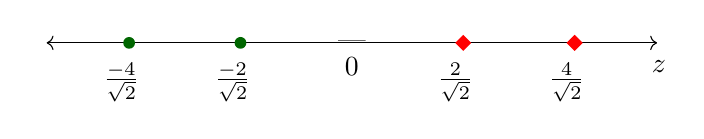
\begin{tikzpicture}
					\node (origin) at (0, 0) {|};
            		%\node (top) at ($(origin) + (0, 4)$) {};
            		%\node (bottom) at ($(origin) + (0, -4)$) {};
            		\node (left) at ($(origin) + (-4, 0)$) {};
            		\node (right) at ($(origin) + (4, 0)$) {};
					\node at ($(origin) + (3.9, -0.3)$) {$z$};
					\node at ($(origin) + (0, -0.3)$) {0};
            		%\draw [->] (bottom) -- (top);
            		\draw [<->] (left) -- (right);

					\node[circle, fill=black!60!green, inner sep=1.5pt] at ($(origin) + (-4/1.414, 0)$) (dp1) {};
					\node at ($(origin) + (-4/1.414 -0.1, -0.5)$) {$\frac{-4}{\sqrt{2}}$};
					\node[circle, fill=black!60!green, inner sep=1.5pt] at ($(origin) + (-2/1.414, 0)$) (dp1) {};
					\node at ($(origin) + (-2/1.414 -0.1, -0.5)$) {$\frac{-2}{\sqrt{2}}$};
					\node[diamond, fill=red, inner sep=1.5pt] at ($(origin) + (2/1.414, 0)$) (dp1) {};
					\node at ($(origin) + (2/1.414 -0.1, -0.5)$) {$\frac{2}{\sqrt{2}}$};
					\node[diamond, fill=red, inner sep=1.5pt] at ($(origin) + (4/1.414, 0)$) (dp1) {};
					\node at ($(origin) + (4/1.414 -0.1, -0.5)$) {$\frac{4}{\sqrt{2}}$};
				\end{tikzpicture}
\end{Described}
				\caption{Plot of Transactions in 1-D}
			\end{figure}
		}

		%Part D:
		
		\qitem	Suppose you are given some transaction datapoint, $\vec{x}_i$ and you project it to be one-dimensional, i.e. $z_i$. \textbf{Based on your plot from part (c), come up with an inequality in terms of $z_i$ to identify if that transaction is fraudulent.}
			
			\textit{Note: There can be more than one answer, but please only give one.}

		\ans{
			$\vec{z}_i > 0$ is a possible answer. In fact any answer in between $\vec{z}_i \geq -\frac{2}{\sqrt{2}}$ and $\vec{z}_i \geq \frac{2}{\sqrt{2}}$ is valid.
		}

		%Part E:
		
		\qitem	It can often be informative to compare our original data with its PCA reconstructions. \textbf{Using PCA, reconstruct $\vec{z}$ back into 2-D as the matrix $\wt{X} \in \mathbb{R}^{2 \times 4}$.}

		\ans{
			Using the reconstruction principle of PCA, we lift the 1D data back into 2 dimensions by doing the following:
			\begin{equation}
				\wt{X} = \vec{u}_1\vec{u}_1^{\top}X = \bmqty{-2 & -1 & 1 & 2 \\ -2 & -1 & 1 & 2}
			\end{equation}
		}

		%Part F:
		
		\qitem	Finally, we visualize our PCA reconstruction. \textbf{On the graph below, draw your first principal component direction (extend it as a solid line in both directions). Draw your reconstructioned points from $\wt{X}$, with dotted lines connecting them with the corresponding point in $X$. } You may draw on the plot on the next page.

			\begin{figure}[H]
				\centering
				\begin{Described}{Scatter plot on x and y axes running about minus 4 to 4, with four transactions marked: circles at (-3, -1) and (0, -2), and diamonds at (2, 0) and (1, 3).}
\begin{tikzpicture}
					\node (origin) at (0, 0) {};
					\node (top) at ($(origin) + (0, 4)$) {};
					\node (bottom) at ($(origin) + (0, -4)$) {};
					\node (left) at ($(origin) + (-4, 0)$) {};
					\node (right) at ($(origin) + (4, 0)$) {};
					\draw [->] (bottom) -- (top);
					\draw [->] (left) -- (right);
			
					\node at (-3, -2.2) (leftendpoint) {};
					\node at (3, 2.2) (rightendpoint) {};
					%\node at ($(origin) + (0.8, 1.3)$) {$y=\alpha x$};
					\node at ($(origin) + (3.9, -0.3)$) {$x$};
					\node at ($(origin) + (0.3, 4.0)$) {$y$};
			
					%\draw[line width=0.75mm] (leftendpoint) -- (rightendpoint);
			
					\node[circle, fill=black!60!green, inner sep=1.5pt] at ($({-3/1.0}, {-1/1.0})$) (dp1) {};
					\node[circle, fill=black!60!green, inner sep=1.5pt] at ($({0/1.0}, {-2/1.0})$) (dp2) {};
					\node[diamond, fill=red, inner sep=1.5pt] at ($({1/1.0}, {3/1.0})$) (dp3) {};
					\node[diamond, fill=red, inner sep=1.5pt] at ($({2/1.0}, {0/1.0})$) (dp4) {};
			
					\node at ($({1/1.0}, 0.1)$) (dp1x) {};
					\node at ($(-0.1, {-2/1.0})$) (dp1y) {};
					\node at ($({1/1.0}, 0.3)$) {$1$};
					\node at ($(-0.3, {-2/1.0})$) {$-2$};
					%\draw[dotted] (dp1) -- (dp1x);
					%\draw[dotted] (dp1) -- (dp1y);
			
					\node at ($({2/1.0}, -0.1)$) (dp2x) {};
					\node at ($(-0.1, {3/1.0})$) (dp2y) {};
					\node at ($({2/1.0}, -0.3)$) {$2$};
					\node at ($(-0.3, {3/1.0})$) {$3$};
					%\draw[dotted] (dp2) -- (dp2x);
					%\draw[dotted] (dp2) -- (dp2y);
			
					\node at ($({-3/1.0}, 0.1)$) (dp3x) {};
					\node at ($(0.1, {-1/1.0})$) (dp3y) {};
					\node at ($({-3/1.0}, 0.3)$) {$-3$};
					\node at ($(-0.3, {-1/1.0 -0.3} )$) {$-1$};
					%\draw[dotted] (dp3) -- (dp3x);
					%\draw[dotted] (dp3) -- (dp3y);
			
			
					\node[inner sep=0pt] at ($(leftendpoint)!(dp1)!(rightendpoint)$) (pdp1) {};
					\node[inner sep=0pt] at ($(leftendpoint)!(dp2)!(rightendpoint)$) (pdp2) {};
					\node[inner sep=0pt] at ($(leftendpoint)!(dp3)!(rightendpoint)$) (pdp3) {};
			
					%\draw[red] (dp1) -- (pdp1);
					%\draw[red] (dp2) -- (pdp2);
					%\draw[red] (dp3) -- (pdp3);
				\end{tikzpicture}
\end{Described}
				\caption{Plot of Transactions in 2-D}
			\end{figure}

		\ans{

			Using the answer from part (d), students should end up with the following graph:
			\begin{figure}[H]
				\centering
				\begin{Described}{The same four transactions, with a solid line through the origin along y = x and reconstructed points on it at (-2, -2), (-1, -1), (1, 1) and (2, 2), each joined to its original point by a dotted line.}
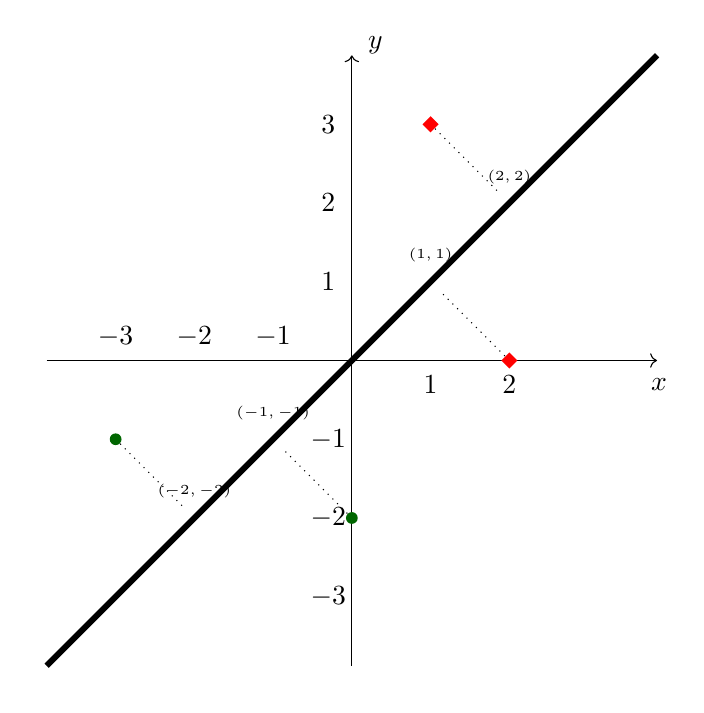
\begin{tikzpicture}
					\node (origin) at (0, 0) {};
					\node (top) at ($(origin) + (0, 4)$) {};
					\node (bottom) at ($(origin) + (0, -4)$) {};
					\node (left) at ($(origin) + (-4, 0)$) {};
					\node (right) at ($(origin) + (4, 0)$) {};
					\draw [->] (bottom) -- (top);
					\draw [->] (left) -- (right);
			
					\node at (-4, -4) (leftendpoint) {};
					\node at (4, 4) (rightendpoint) {};
					%\node at ($(origin) + (0.8, 1.3)$) {$y=\alpha x$};
					\node at ($(origin) + (3.9, -0.3)$) {$x$};
					\node at ($(origin) + (0.3, 4.0)$) {$y$};
			
					\draw[line width=0.75mm] (leftendpoint) -- (rightendpoint);
			
					\node[circle, fill=black!60!green, inner sep=1.5pt] at ($({-3/1.0}, {-1/1.0})$) (dp1) {};
					\node[circle, fill=black!60!green, inner sep=1.5pt] at ($({0/1.0}, {-2/1.0})$) (dp2) {};
					\node[diamond, fill=red, inner sep=1.5pt] at ($({2/1.0}, {0/1.0})$) (dp3) {};
					\node[diamond, fill=red, inner sep=1.5pt] at ($({1/1.0}, {3/1.0})$) (dp4) {};
					

					\node[label= {\tiny $\left( -2, -2\right)$}] at (-2, -2) (r1) {};
					\node[label= {\tiny $\left( -1, -1\right)$}] at (-1, -1) (r2) {};
					\node[label= {\tiny $\left( 1, 1\right)$}] at (1, 1) (r3) {};
					\node[label= {\tiny $\left( 2, 2\right)$}] at (2, 2) (r4) {};

					\draw[dotted] (dp1) -- (r1);
					\draw[dotted] (dp2) -- (r2);
					\draw[dotted] (dp3) -- (r3);
					\draw[dotted] (dp4) -- (r4);
			
					\node at ($({1/1.0}, 0.1)$) (dp1x) {};
					\node at ($(-0.1, {-2/1.0})$) (dp1y) {};
					\node at ($({1/1.0}, -0.3)$) {$1$};
					\node at ($(-0.3, {-2/1.0})$) {$-2$};
					%\draw[dotted] (dp1) -- (dp1x);
					%\draw[dotted] (dp1) -- (dp1y);
			
					\node at ($({2/1.0}, -0.1)$) (dp2x) {};
					\node at ($(-0.1, {3/1.0})$) (dp2y) {};
					\node at ($({2/1.0}, -0.3)$) {$2$};
					\node at ($(-0.3, {1/1.0})$) {$1$};
					\node at ($(-0.3, {2/1.0})$) {$2$};
					\node at ($(-0.3, {3/1.0})$) {$3$};
					%\draw[dotted] (dp2) -- (dp2x);
					%\draw[dotted] (dp2) -- (dp2y);
			
					\node at ($({-3/1.0}, 0.1)$) (dp3x) {};
					\node at ($(0.1, {-1/1.0})$) (dp3y) {};
					\node at ($({-3/1.0}, 0.3)$) {$-3$};
					\node at ($({-2/1.0}, 0.3)$) {$-2$};
					\node at ($({-1/1.0}, 0.3)$) {$-1$};
					\node at ($(-0.3, {-3/1.0} )$) {$-3$};
					\node at ($(-0.3, {-1/1.0} )$) {$-1$};
					%\draw[dotted] (dp3) -- (dp3x);
					%\draw[dotted] (dp3) -- (dp3y);
			
			
					\node[inner sep=0pt] at ($(leftendpoint)!(dp1)!(rightendpoint)$) (pdp1) {};
					\node[inner sep=0pt] at ($(leftendpoint)!(dp2)!(rightendpoint)$) (pdp2) {};
					\node[inner sep=0pt] at ($(leftendpoint)!(dp3)!(rightendpoint)$) (pdp3) {};
			
					%\draw[red] (dp1) -- (pdp1);
					%\draw[red] (dp2) -- (pdp2);
					%\draw[red] (dp3) -- (pdp3);
				\end{tikzpicture}
\end{Described}
				\caption{Plot of Transactions in 2-D}
			\end{figure}
		}


\end{enumerate}

  \newpage
  \qns{Diode System ID (Adapted from EECS 16B Fall 2023 Final)}

    \textbf{Note: This problem does not require knowledge of circuits or diodes.}
    
    Suppose that we want to characterize a diode $D_1$ with parasitic resistance $R_p$, represented by the following model:
    \begin{figure}[H]
        \begin{center}
            \begin{Described}{Voltage source V sub B drives from ground up to the top node, where diode D1 carries current I D to the right with voltage V D across it, in series with resistor R sub p returning to ground.}
\begin{circuitikz}
                \draw (0, 2) to [V, l_=$V_B$] (0, 0) node[ground]{}
                (0, 2) to [Do, l=$D_1$, i=$I_D$, v=$V_D$] (3, 2) to [R, l=$R_p$] (5, 2) node[ground]{}
                ;
            \end{circuitikz}
\end{Described}
        \end{center}
    \end{figure}
    The current through the diode (forward-biased) is modeled as
    \begin{equation}
        I_D = I_0\e^{\frac{V_D}{V_T}}
    \end{equation}
    where $V_D$ is the voltage across the diode (as shown in the diagram), $I_0$ is a parameter associated with the diode, and $V_T$ is the thermal voltage, a temperature dependent variable.
    
    With some analysis, the system equation can be simplified to:
    \begin{equation}
        I_D = I_0 \e^{\frac{V_B - I_D R_p}{V_T}}
    \end{equation}
    To collect data, we will vary the temperature to vary $V_T$ and measure the current $I_D$ through the diode.
    
        \begin{enumerate}

            \qitem    Use the provided system equation to show that
                \begin{equation}
                    I_D R_p - V_T \ln(I_0) = V_B - V_T \ln(I_D)
                \end{equation}
                    is a valid equation to represent the system.
                \begin{hint}
                    Use the logarithm identity $\ln(\frac{a}{b}) = \ln(a) - \ln(b)$.
                \end{hint}
            
    
            \ans{
                \begin{align}
                    I_D &= I_0 \e^{\frac{V_B - I_D R_p}{V_T}} \\
                    V_T\ln(\frac{I_D}{I_0}) &= V_B - I_D R_p \\
                    V_T\ln(I_D) - V_T\ln(I_0) &= V_B - I_D R_p \\
                    I_D R_p - V_T \ln(I_0) &= V_B - V_T \ln(I_D)
                \end{align}
            }
    
            % \begin{problempart}{4}{System ID}{0}{0}
            %     Suppose we use $V_B = 1 \mathrm{V}$ and collect the following data points:
            %     \begin{itemize}
            %         \item For $V_T = 0.025 \mathrm{V}$, $I_D = 0.0185 \mathrm{A}$.
            %         \item For $V_T = 0.05 \mathrm{V}$, $I_D = 0.0172 \mathrm{A}$.
            %         \item For $V_T = 0.0125 \mathrm{V}$, $I_D = 0.0193 \mathrm{A}$.
            %     \end{itemize}
            %     \textbf{Find the matrix $D$ and vector $\vec{s}$ to set up a least-squares problem $D\vec{p} \approx \vec{s}$ where $\vec{p} = \begin{bmatrix} \ln(I_0) \\ R_p \end{bmatrix}$.}
    
            %     You do not have to simplify the elements $D$ and $\vec{s}$, but the elements should be numerical values, not in terms of variables.
            % \end{problempart}
    
            % \begin{solution}{4in}
            %     Each data point can be used with the provided system equation from the first part to create a system of linear equations with the unknowns being $\ln(I_0)$ and $R_p$ (remember that the problem provides that $V_B = 1 \mathrm{V}$):
            %     \begin{itemize}
            %         \item $-0.025\ln(I_0) + 0.0185R_p = 1 - 0.025\ln(0.0185)$
            %         \item $-0.05\ln(I_0) + 0.0172R_p = 1 - 0.05\ln(0.0172)$
            %         \item $-0.0125\ln(I_0) + 0.0193R_p = 1 - 0.0125\ln(0.0193)$
            %     \end{itemize}
            %     The matrix form of this system is:
            %     \begin{equation}
            %         \begin{bmatrix} -0.025 & 0.0185 \\ -0.05 & 0.0172 \\ -0.0125 & 0.0193 \end{bmatrix} \begin{bmatrix} \ln(I_0) \\ R_p \end{bmatrix} = \begin{bmatrix} 1 - 0.025\ln(0.0185) \\ 1 - 0.05\ln(0.0172) \\ 1 - 0.0125\ln(0.0193) \end{bmatrix}
            %     \end{equation}
            %     Thus, for the least-squares problem, $D = \begin{bmatrix} -0.025 & 0.0185 \\ -0.05 & 0.0172 \\ -0.0125 & 0.0193 \end{bmatrix}$ and $\vec{s} = \begin{bmatrix} 1 - 0.025\ln(0.0185) \\ 1 - 0.05\ln(0.0172) \\ 1 - 0.0125\ln(0.0193) \end{bmatrix}$
            % \end{solution}
    
            \vspace{5cm}
            
            \qitem    Suppose we use $V_B = v_B$ and collect the following data points:
                \begin{itemize}
                    \item For $V_T = v_{T1}$, $I_D = i_{D1}$.
                    \item For $V_T = v_{T2}$, $I_D = i_{D2}$.
                    \item For $V_T = v_{T3}$, $I_D = i_{D3}$.
                \end{itemize}
                Find the matrix $\textbf{A}$ and vector $\vec{x}$ to set up a least-squares problem $\textbf{A} \vec{x} \approx \vec{b}$ where $\vec{x} = \begin{bmatrix} \ln(I_0) \\ R_p \end{bmatrix}$
    
            \ans{
                Each data point can be used with the provided system equation from the first part to create a system of linear equations with the unknowns being $\ln(I_0)$ and $R_p$ (remember that the problem provides that $V_B = v_B$):
                \begin{itemize}
                    \item $-v_{T1}\ln(I_0) + i_{D1}R_p = v_B - v_{T1}\ln(i_{D1})$
                    \item $-v_{T2}\ln(I_0) + i_{D2}R_p = v_B - v_{T2}\ln(i_{D2})$
                    \item $-v_{T3}\ln(I_0) + i_{D3}R_p = v_B - v_{T3}\ln(i_{D3})$
                \end{itemize}
                The matrix form of this system is:
                \begin{equation}
                    \begin{bmatrix} -v_{T1} & i_{D1} \\ -v_{T2} & i_{D2} \\ -v_{T3} & i_{D3} \end{bmatrix} \begin{bmatrix} \ln(I_0) \\ R_p \end{bmatrix} = \begin{bmatrix} v_B - v_{T1}\ln(i_{D1}) \\ v_B - v_{T2}\ln(i_{D2}) \\ v_B - v_{T3}\ln(i_{D3}) \end{bmatrix}
                \end{equation}
                Thus, for the least-squares problem, $\textbf{A} = \begin{bmatrix} -v_{T1} & i_{D1} \\ -v_{T2} & i_{D2} \\ -v_{T3} & i_{D3} \end{bmatrix}$ and $\vec{b} = \begin{bmatrix} v_B - v_{T1}\ln(i_{D1}) \\ v_B - v_{T2}\ln(i_{D2}) \\ v_B - v_{T3}\ln(i_{D3}) \end{bmatrix}$
            }
            
            \vspace{5cm}
            
            \qitem    Explain how you would use the least-squares system from the previous part to find model parameters $I_0$ and $R_p$. You do not need to use actual values for this part; you explanation can just use $\textbf{A}$ and $\vec{b}$ as known variables to show what calculations you would do to find $I_0$ and $R_p$.
            
    
            \ans{
                We would first find the optimal parameter $\hat{\vec{x}}$ with the least squares formula:
                \begin{equation}
                    \hat{\vec{x}} = (\textbf{A}^\top \textbf{A})^{-1} \textbf{A}^{\top} \vec{b}
                \end{equation}
                The elements of $\hat{\vec{x}}$ represent optimal values for $\ln(I_0)$ and $R_p$ so we set the elements of $\hat{\vec{x}}$ equal to those parameters for our model:
                \begin{align}
                    \hat{x}_{v_B} = \ln(I_0) &\rightarrow I_0 = \e^{\hat{x}_1} \\
                    \hat{x}_2 = R_p &\rightarrow R_p = \hat{x}_2
                \end{align}
                Thus, we have found parameter values for $I_0$ and $R_p$ from the least-squares system.
            }
    
        \end{enumerate}

\end{qunlist}

\end{document}
"

\DocumentMetadata{
  lang       = en-US,
  pdfversion = 2.0,
  testphase  = {phase-III,math,table,graphic,firstaid},
}
\documentclass{latexally-assignment}

\usepackage{amsmath,amssymb}
\usepackage{float}
\usepackage{tikz}
\usetikzlibrary{calc,shapes.geometric,positioning}
\usepackage[american]{circuitikz}

% The corpus macros these four files use, reproduced from questionBank/ee16.sty
% and questionBank/sp26/sp26.sty so the demo does not need the whole course
% preamble chain. Same meanings, nothing more.
\providecommand{\bmqty}[1]{\begin{bmatrix}#1\end{bmatrix}}
\providecommand{\e}{\mathop{\mathrm{e}}\nolimits}
\providecommand{\wt}[1]{\widetilde{#1}}
\NewDocumentEnvironment{hint}{+b}{\itshape (HINT: #1)}{}

\setcoursenumber{EECS 16A}
\setcoursename{Designing Information Devices and Systems I}
\setsemester{Spring 2026}

\begin{document}

\def\title{Described figures from the question bank}
\maketitle

\vspace{0.5em}
Every figure below carries a description in the PDF structure tree. A screen
reader announces "graphic" and then that description; it never reaches the
drawing underneath. Hovering shows nothing --- \texttt{/Alt} is not a tooltip.

\begin{qunlist}

  \qns{Polynomial Multiplication and Discrete-Time Convolution [Adapted from EE 120]}
% Adapted and extended by Ken Zheng for EECS 16A Fall 2025 Discussion

The impulse response of a real, discrete-time FIR filter $\mathsf{A}$ is described by  
$$a[n]=a_0 \delta[n]+a_1 \delta[n-1]+\cdots + a_N \delta[n-N], \quad \text{where } N\in \{1,2,3,\ldots\}.$$

\begin{enumerate}[(a)]
\item Show that the frequency response $A(\omega)$ of the filter is a polynomial, in terms of $e^{-i\omega}$, whose coefficients have a simple relationship with the impulse response values $a_0,\ldots,a_N$.

\ans{

    Substituting \(a[n]\) into the frequency response formula we see that:
    \begin{equation*}
        A(w) = \sum_{n=-\infty}^{\infty} a[n]e^{-iwn}
    \end{equation*}
    As $a[n] = 0$ outside the range of $n = 0$ to $n = N$ ,
    \begin{equation*}
        A(w) = a_0 e^{-iw\cdot 0} + a_1 e^{-iw\cdot 1} + \ldots + a_N e^{-iw\cdot N}
    \end{equation*}
    \begin{equation*}
        = a_0 + a_1 e^{-iw} + \ldots + a_N e^{-iwN}
    \end{equation*}
}
\item Suppose the filter $\mathsf{A}$ is placed in a cascade (series) interconnection with another discrete-time FIR filter $\mathsf{B}$ whose impulse response is described by  
$$b[n]=b_0 \delta[n]+b_1 \delta[n-1]+\cdots + b_M \delta[n-M],\quad \text{where } M\in \{1,2,3,\ldots\}.$$

The cascade structure, which we call $\mathsf{C}$, is shown in the figure below.
\vspace{4pt}

\centerline{
    \begin{Described}{Block diagram: input x enters block A, whose output feeds block B, and block B's output is y. An outer box enclosing both blocks is labelled C.}
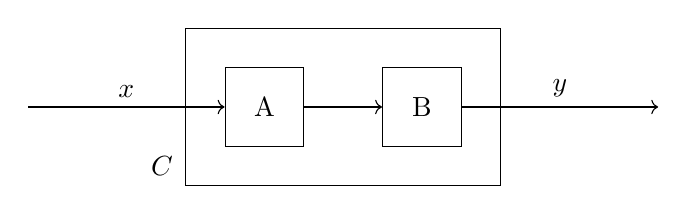
\begin{tikzpicture}
        % Define nodes for blocks A and B
        \node[draw, rectangle, minimum width=1cm, minimum height=1cm] (A) at (0,0) {A};
        \node[draw, rectangle, minimum width=1cm, minimum height=1cm] (B) at (2,0) {B};
        
        % Draw the outer rectangle
        \draw (-1, 1) rectangle (3, -1);
        
        % Draw arrows and labels
        \draw[->] (-3, 0) -- (A.west) node[midway,above] {$x$};
        \draw[->] (A.east) -- (B.west);
        \draw[->] (B.east) -- (5, 0) node[midway,above] {$y$};
        
        % Label C 
        \node at (-1.3, -0.5) [below] {$C$};
    \end{tikzpicture}
\end{Described}
}
Let $c$ denote the impulse response of the cascade interconnection.

\begin{enumerate}[(i)]
\item Express $c$ in terms of $a$ and $b$.
    
\ans{

        The impulse response \(c\) of the cascade interconnection is given by 
        \begin{equation*}
            c[n] = (a * b)[n] = \sum_{k=-\infty}^{\infty} a[k]\,b[n-k]
        \end{equation*}
         Substituting \(n = 0\):
        \begin{equation*}
            c_0 = a_0 b_0
        \end{equation*}
        \(n = 1\):
        \begin{equation*}
            c_1 = a_0 b_1 + a_1 b_0 
        \end{equation*}
        \(n = 2\):
        \begin{equation*}
            c_2 = a_0 b_2 + a_1 b_1 + a_2 b_0
        \end{equation*}
        And so on...
    
        Thus, we can write:
        \begin{equation*}
            c_n = \sum_{k=\max(0,n-M)}^{\min(n, N)} a_k b_{n-k}
        \end{equation*}
        \null\hfill for \(n = 0, 1, \ldots, N + M\)
        
        where we found the bounds of summation from the two conditions that ensure we are indexing \(a[n]\) and \(b[n]\) without exceeding the bounds of their signal.
        $$ 0 \leq k \leq N \Longrightarrow k \leq N \quad \text{and} \quad k \geq 0 $$
        $$ 0 \leq n - k \leq M \Longrightarrow k \leq n \quad \text{and} \quad k \geq n - M $$
        and so
        $$ k \leq \min(n, N) \quad \text{and} \quad k \geq \max(0, n-M) $$

        Lastly, 
         \begin{equation*}
            c[n] = c_0\delta[n] + c_1 \delta[n - 1] + ... + c_{N + M} \delta[n - ( N + M)]
        \end{equation*}
        
    }

\item Consider two polynomials $A(z)$ and $B(z)$ described as follows:
    $$
    A(z) = a_0 +a_1 z + \cdots + a_N z^N \quad \quad \quad B(z) = b_0 +b_1 z + \cdots + b_M z^M \, ,
    $$
    where $M$ and $N$ and positive integers.
    Let $C(z)=A(z)\, B(z)$, where $$ C(z) = c_0 +c_1 z + \cdots + c_{N+M} z^{N+M}.$$  Show that multiplying polynomials is tantamount to convolving their coefficients; in particular, explain how $c_n=(a*b)_n=\displaystyle\sum_m a_m b_{n-m}$, where $n={0,1,\ldots, N+M}$.
    
    \ans{
    \begin{equation*}
        C(z) = (a_0 +a_1 z + \cdots + a_N z^N) (b_0 +b_1 z + \cdots + b_M z^M)
    \end{equation*}
    \begin{equation*}
        C(z) = a_0 b_0 + (a_0 b_1 + a_1 b_0) z + (a_0 b_2 + a_1 b_1 + a_2 b_0) z^2 + ...
    \end{equation*}
    As you can see, each coefficient of \(z^n\) is the sum of all products of \(a_i\) and \(b_j\) where \(i + j = n\):
    \begin{equation*}
        c_n =  \sum_{m=\max(0,n-M)}^{\min(n, N)} a_m b_{n-m}
    \end{equation*}
    \null\hfill for \(n = 0, 1, 2, ..., N + M\)

    Just like the definition of convolution!
    }

\end{enumerate}
\end{enumerate}
  \newpage
  \qns{Frequency Response from a DAG Block Diagram [Adapted from EE 120]}
% Adapted by Ken Zheng for EECS 16A Fall 2025 Discussion

    Consider a DT LTI system with input $x[n]$ and output $y[n]$ that is implemented by the following block diagram:
    \begin{figure}[h!]
      \centering
      \begin{Described}{Block diagram: input x of n enters a summing junction whose output is y of n. That output is tapped, passed through a delay block D and then a gain of minus 0.5, and fed back into the summing junction.}
\begin{circuitikz}
          \node (x) at (0, 0) {$x[n]$};
          \node[circle, draw] (sum) at (2, 0) {$+$};
          % FIXME: find a better way to draw the triangle
          % \node[triangleblock, shape border rotate=90, inner sep=-1mm] (gain) at (3, -1.5) {$-0.5$};
          % \node at (3, -1.5) {$-0.5$};
          \node[draw, inner sep=5pt] (delay) at (6, -1.5) {$D$};
          \node (y) at (9, 0) {$y[n]$};
          \draw[->] (x.east) -- (sum.west);
          \draw[->] (sum.east) -- (y.west);
          \draw[->] (7.5, 0) -- (7.5, -1.5) -- (delay.east);
          % \draw[-, thick] (delay.west) -- (gain.east);
          % \draw[->, thick] (gain.west) -- (2, -1.5) -- (sum.south);
          \draw[->] (delay.west) to [amp, t=$-0.5$, blocks/scale=1.5] (2, -1.5) to (sum.south);
      \end{circuitikz}
\end{Described}
  \end{figure}
\begin{enumerate}
        \item Find the LCCDE that describes this system. 
        
        \ans{
            The difference equation describing this system is
              \begin{equation*}
                y[n] = x[n] - 0.5y[n-1]
              \end{equation*}
        }

        \item Find the frequency response $H(\omega)$ of this system. 
            
        \ans{
            Using the eigenfunction property by setting $x[n] = e^{i\omega n}$ and $y[n] = H(\omega) e^{i\omega n}$,
            \begin{align*}
            H(\omega) e^{i\omega n} &= e^{i\omega n} - 0.5 H(\omega) e^{i\omega (n-1)} \\
            &= e^{i\omega n} - 0.5 H(\omega) e^{-i\omega}e^{i\omega n} \\
            \left(1 + 0.5 e^{-i\omega}\right) e^{i\omega n} H(\omega) &= e^{i\omega n} \\
            H(\omega) &= \frac{e^{i\omega n}}{\left(1 + 0.5 e^{-i\omega}\right)e^{i\omega n}} \\
                &= \frac{1}{1 + 0.5 e^{-i\omega}}
            \end{align*} 
        } 

        \vspace{4cm}

        \item Is this a high pass or low pass filter?
        
        \ans{
            We can think about this in two ways:
            
            \textbf{1. Geometric Approach:}

            Recall from part (b) that the frequency response can be written as:
            \[
            H(\omega) = \frac{1}{1 + 0.5 e^{-i\omega}} = \frac{e^{i\omega}}{e^{i\omega} - (-0.5)}
            \]
            The magnitude is therefore:
            \[
            |H(\omega)| = \frac{1}{|e^{i\omega} - (-0.5)|}
            \]
            This represents the reciprocal of the distance from the point $e^{i\omega}$ on the unit circle to the point located at $-0.5$ on the real axis:

            \begin{center}
            \begin{Described}{Complex plane with real and imaginary axes and the unit circle centred at the origin. A point is marked at minus 0.5 on the real axis, with an arrow from it to the point e to the i omega on the circle.}
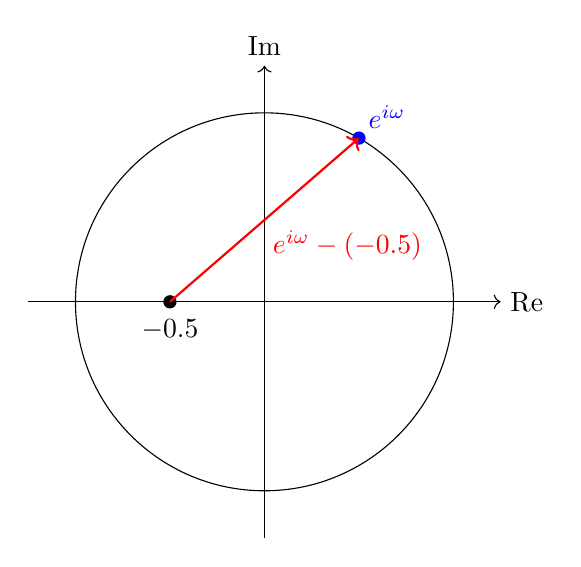
\begin{tikzpicture}[scale=1.2]
                % Axes
                \draw[->] (-2.5,0) -- (2.5,0) node[right] {$\operatorname{Re}$};
                \draw[->] (0,-2.5) -- (0,2.5) node[above] {$\operatorname{Im}$};

                % Unit circle
                \draw (0,0) circle (2);

                % Pole at -0.5
                \fill[black] (-1,0) circle (2pt) node[below left] {};
                \node[black] at (-1,-0.3) {$-0.5$};

                % Point on unit circle at angle ω
                \coordinate (P) at (60:2);
                \fill[blue] (P) circle (2pt) node[above right] {$e^{i\omega}$};

                % Vector from pole to point on circle
                % \draw[->, thick, red] (-1,0) -- (P);
                \draw[->, thick, red] (-1,0) -- (P) node[midway, below] {$\qquad\qquad\qquad e^{i \omega} - (-0.5)$};  % Label added here


                % Labels
                \node at (1.8,1.8) {};
            \end{tikzpicture}
\end{Described}
            \end{center}

            Key observations:
            \begin{itemize}
                \item When $\omega = 0$, $e^{i\omega} = 1$. The distance from $1$ to $-0.5$ is $1.5$, so $|H(0)| = 1/1.5 \approx 0.667$.
                \item When $\omega = \pi$, $e^{i\omega} = -1$. The distance from $-1$ to $-0.5$ is $0.5$, so $|H(\pi)| = 1/0.5 = 2$.
                \item As $\omega$ moves from $0$ to $\pi$, the point $e^{i\omega}$ travels along the upper half of the unit circle from $(1,0)$ to $(-1,0)$. 
                The distance to the point at $-0.5$ decreases monotonically, so $|H(\omega)|$ increases. Thus, we have a high-pass filter!\\
            \end{itemize}

            
            \textbf{2. Algebraic Approach:}
            
            To determine the filter type, we simplify the magnitude of the frequency response first:

            \[
            |H(\omega)| = \frac{1}{\sqrt{(1 + 0.5\cos\omega)^2 + (0.5\sin\omega)^2}}
            \]


            Expanding \( (1 + 0.5\cos\omega)^2 \) and \( (0.5\sin\omega)^2 \):
            \[
            (1 + 0.5\cos\omega)^2 = 1^2 + 2(1)(0.5\cos\omega) + (0.5\cos\omega)^2 = 1 + \cos\omega + 0.25\cos^2\omega
            \]
            \[
            (0.5\sin\omega)^2 = 0.25\sin^2\omega
            \]


            Add the two results in the square root:
            \[
            (1 + 0.5\cos\omega)^2 + (0.5\sin\omega)^2 = \left[1 + \cos\omega + 0.25\cos^2\omega\right] + \left[0.25\sin^2\omega\right]
            \]
            \[
            = 1 + \cos\omega + 0.25\left(\cos^2\omega + \sin^2\omega\right)
            \]
            \[
            = 1 + \cos\omega + 0.25(1) = 1 + \cos\omega + 0.25 = 1.25 + \cos\omega
            \]


            Substitute back into \( |H(\omega)| \):
            \[
            |H(\omega)| = \frac{1}{\sqrt{1.25 + \cos\omega}}
            \]
                        
            Now we analyze the magnitude at key frequencies:
            
            Low frequency (\( \omega = 0 \)): 
                \[
                |H(0)| =  \frac{1}{\sqrt{1.25 + \cos0}} = \frac{1}{1.5} \approx 0.667 \quad (\text{attenuated})
                \]
            High frequency (\( \omega = \pi \)): 
                \[
                |H(\pi)| =  \frac{1}{\sqrt{1.25 + \cos\pi}} = 2 \quad (\text{passed})
                \]

            We can see that, again, the filter attenuates low frequencies and passes high frequencies, so it is a high-pass filter!\\

            Both geometrically and algebraically, we conclude this is a \textbf{high-pass filter}. Nice!
        }
\end{enumerate}

  \newpage
  \qns{Using PCA to Detect Fraudulent Transactions (Adapted from EECS 16B Spring 2023 Final)}\\
	PCA has many different uses when applied to real-world data. One potential application is making classification of data much easier.
	
	Suppose we are given some data, where each datapoint represents a transaction. Each one is labeled either normal or fraudulent. We will utilize PCA to develop a useful classifier.

	We plot the data in two dimensions, where each dimension is some unspecified feature that will aid us in classifying the points:

	\begin{figure}[H]
        \centering
        \begin{Described}{Scatter plot on x and y axes running about minus 4 to 4, with four transactions marked: circles at (-3, -1) and (0, -2), and diamonds at (2, 0) and (1, 3).}
\begin{tikzpicture}
            \node (origin) at (0, 0) {};
            \node (top) at ($(origin) + (0, 4)$) {};
            \node (bottom) at ($(origin) + (0, -4)$) {};
            \node (left) at ($(origin) + (-4, 0)$) {};
            \node (right) at ($(origin) + (4, 0)$) {};
            \draw [->] (bottom) -- (top);
            \draw [->] (left) -- (right);
    
            \node at (-3, -2.2) (leftendpoint) {};
            \node at (3, 2.2) (rightendpoint) {};
            %\node at ($(origin) + (0.8, 1.3)$) {$y=\alpha x$};
            \node at ($(origin) + (3.9, -0.3)$) {$x$};
            \node at ($(origin) + (0.3, 4.0)$) {$y$};
    
            %\draw[line width=0.75mm] (leftendpoint) -- (rightendpoint);
    
            \node[circle, fill=black!60!green, inner sep=1.5pt] at ($({-3/1.0}, {-1/1.0})$) (dp1) {};
            \node[circle, fill=black!60!green, inner sep=1.5pt] at ($({0/1.0}, {-2/1.0})$) (dp2) {};
            \node[diamond, fill=red, inner sep=1.5pt] at ($({1/1.0}, {3/1.0})$) (dp3) {};
			\node[diamond, fill=red, inner sep=1.5pt] at ($({2/1.0}, {0/1.0})$) (dp4) {};
    
            \node at ($({1/1.0}, 0.1)$) (dp1x) {};
            \node at ($(-0.1, {-2/1.0})$) (dp1y) {};
            \node at ($({1/1.0}, 0.3)$) {$1$};
            \node at ($(-0.3, {-2/1.0})$) {$-2$};
            %\draw[dotted] (dp1) -- (dp1x);
            %\draw[dotted] (dp1) -- (dp1y);
    
            \node at ($({2/1.0}, -0.1)$) (dp2x) {};
            \node at ($(-0.1, {3/1.0})$) (dp2y) {};
            \node at ($({2/1.0}, -0.3)$) {$2$};
            \node at ($(-0.3, {3/1.0})$) {$3$};
            %\draw[dotted] (dp2) -- (dp2x);
            %\draw[dotted] (dp2) -- (dp2y);
    
            \node at ($({-3/1.0}, 0.1)$) (dp3x) {};
            \node at ($(0.1, {-1/1.0})$) (dp3y) {};
            \node at ($({-3/1.0}, 0.3)$) {$-3$};
            \node at ($(-0.3, {-1/1.0 -0.3} )$) {$-1$};
            %\draw[dotted] (dp3) -- (dp3x);
            %\draw[dotted] (dp3) -- (dp3y);
    
    
            \node[inner sep=0pt] at ($(leftendpoint)!(dp1)!(rightendpoint)$) (pdp1) {};
            \node[inner sep=0pt] at ($(leftendpoint)!(dp2)!(rightendpoint)$) (pdp2) {};
            \node[inner sep=0pt] at ($(leftendpoint)!(dp3)!(rightendpoint)$) (pdp3) {};
    
            %\draw[red] (dp1) -- (pdp1);
            %\draw[red] (dp2) -- (pdp2);
            %\draw[red] (dp3) -- (pdp3);
        \end{tikzpicture}
\end{Described}
        \caption{Plot of Transactions in 2-D}
	\end{figure}

	Thus, we have a total of 4 transactions, $\bmqty{-3 \\ -1}$ and $\bmqty{0 \\ -2}$ are normal, while $\bmqty{2 \\ 0}$ and $\bmqty{1 \\ 3}$ are fraudulent.
	\begin{enumerate}
		%Part A:
		
		\qitem Suppose we now construct a data matrix, where the \textit{data points are columns}. 

			\begin{equation}
				X = \bmqty{-3 & 0 & 2 & 1 \\ -1 & -2 & 0 & 3}
			\end{equation}

			Using this data matrix, \textbf{calculate its first principal component $\vec{u}_1$}.

			\begin{hint}
			\begin{enumerate}

				\item You may also make use of the fact that $XX^T$ is given by:
				\begin{align}
					XX^{\top} &= \bmqty{-3 & 0 & 2 & 1 \\ -1 & -2 & 0 & 3}\bmqty{-3 & 0 & 2 & 1 \\ -1 & -2 & 0 & 3}^{\top} \\
						&= \bmqty{14 & 6 \\ 6 & 14}
				\end{align}
				\item You may also make use of the characteristic polynomial of $XX^T$:
				\begin{equation}
					\lambda^2 - 28\lambda + 160 = (\lambda - 20)(\lambda - 8) = 0
				\end{equation}
			\end{enumerate}
			\end{hint}
			
			\begin{hint} Remember that your principal component should be of unit norm. \end{hint}

		\ans{
			% From PCA, we know that our first principal component of a matrix with column data is the first column vector of $U$ in the SVD of $X$. Thus, we use the SVD method of calculation (find the eigenvector corresponding to the largest eigenvalue of $XX^{\top}$ and normalize to yield $\vec{u}_1$).

			% \begin{align}
			% 	XX^{\top} &= \bmqty{-3 & 0 & 2 & 1 \\ -1 & -2 & 0 & 3}\bmqty{-3 & 0 & 2 & 1 \\ -1 & -2 & 0 & 3}^{\top} \\
			% 		 &= \bmqty{14 & 6 \\ 6 & 14}
			% \end{align}

			% From setting $\mathrm{det}(XX^{\top} - \lambda I) = 0$, we should find our characteristic polynomial to be 
			
			% \begin{equation}
			% 	\lambda^2 - 28\lambda + 160 = 0
			% \end{equation}

			Our eigenvalues are $\lambda_1 = 20$ and $\lambda_2 = 8$. Thus, the eigenvector corresponding to our largest eigenvalue $\lambda_1 = 20$ is $\vec{v}_1 = \bmqty{1 \\ 1}$ from inspection.
			
			Thus, our principal component vector is given as the normalized eigenvector: i.e. $\vec{u}_1 = \bmqty{\frac{1}{\sqrt{2}} \\ \frac{1}{\sqrt{2}}}$.
        }

		%Part B:
		
		\qitem	It's difficult to come up with a useful classifier in two dimensions. Let's use PCA dimensionality reduction to help.
			
			Using your answer in part (a), \textbf{project your two-dimensional data points onto one dimension. Express your answer as the vector $\vec{z} \in \mathbb{R}^{1 \times 4}$.}

		\ans{
			To project our 2-d data into 1-d, we project our data matrix onto the first principal component as follows:
			
			\begin{equation}
				\vec{z} = \vec{u}_1^{\top}X = \bmqty{\frac{1}{\sqrt{2}} \\ \frac{1}{\sqrt{2}}} \bmqty{-3 & 0 & 2 & 1 \\ -1 & -2 & 0 & 3} = \bmqty{-\frac{4}{\sqrt{2}} & -\frac{2}{\sqrt{2}} & \frac{2}{\sqrt{2}} & \frac{4}{\sqrt{2}}}
			\end{equation}
		}
		
		%Part C:
		
		\qitem	Now, plot each of these points, on the line below. Indicate the value and label (normal as circle and fraudulent as diamond) for each point.
			
			\textit{Note: your plot doesn't have to be to scale.}

			\begin{figure}[H]
				\centering
				\begin{Described}{Blank horizontal number line labelled z, with only the origin marked 0 and no points plotted.}
\begin{tikzpicture}
					\node (origin) at (0, 0) {|};
            		%\node (top) at ($(origin) + (0, 4)$) {};
            		%\node (bottom) at ($(origin) + (0, -4)$) {};
            		\node (left) at ($(origin) + (-4, 0)$) {};
            		\node (right) at ($(origin) + (4, 0)$) {};
					\node at ($(origin) + (3.9, -0.3)$) {$z$};
					\node at ($(origin) + (0, -0.3)$) {0};
            		%\draw [->] (bottom) -- (top);
            		\draw [<->] (left) -- (right);

				\end{tikzpicture}
\end{Described}
				\caption{Plot of Transactions in 1-D}
			\end{figure}

		\ans{
			\begin{figure}[H]
				\centering
				\begin{Described}{Number line labelled z with the origin marked 0 and four points: circles at minus four over root two and minus two over root two, diamonds at two over root two and four over root two.}
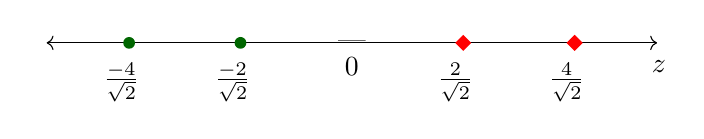
\begin{tikzpicture}
					\node (origin) at (0, 0) {|};
            		%\node (top) at ($(origin) + (0, 4)$) {};
            		%\node (bottom) at ($(origin) + (0, -4)$) {};
            		\node (left) at ($(origin) + (-4, 0)$) {};
            		\node (right) at ($(origin) + (4, 0)$) {};
					\node at ($(origin) + (3.9, -0.3)$) {$z$};
					\node at ($(origin) + (0, -0.3)$) {0};
            		%\draw [->] (bottom) -- (top);
            		\draw [<->] (left) -- (right);

					\node[circle, fill=black!60!green, inner sep=1.5pt] at ($(origin) + (-4/1.414, 0)$) (dp1) {};
					\node at ($(origin) + (-4/1.414 -0.1, -0.5)$) {$\frac{-4}{\sqrt{2}}$};
					\node[circle, fill=black!60!green, inner sep=1.5pt] at ($(origin) + (-2/1.414, 0)$) (dp1) {};
					\node at ($(origin) + (-2/1.414 -0.1, -0.5)$) {$\frac{-2}{\sqrt{2}}$};
					\node[diamond, fill=red, inner sep=1.5pt] at ($(origin) + (2/1.414, 0)$) (dp1) {};
					\node at ($(origin) + (2/1.414 -0.1, -0.5)$) {$\frac{2}{\sqrt{2}}$};
					\node[diamond, fill=red, inner sep=1.5pt] at ($(origin) + (4/1.414, 0)$) (dp1) {};
					\node at ($(origin) + (4/1.414 -0.1, -0.5)$) {$\frac{4}{\sqrt{2}}$};
				\end{tikzpicture}
\end{Described}
				\caption{Plot of Transactions in 1-D}
			\end{figure}
		}

		%Part D:
		
		\qitem	Suppose you are given some transaction datapoint, $\vec{x}_i$ and you project it to be one-dimensional, i.e. $z_i$. \textbf{Based on your plot from part (c), come up with an inequality in terms of $z_i$ to identify if that transaction is fraudulent.}
			
			\textit{Note: There can be more than one answer, but please only give one.}

		\ans{
			$\vec{z}_i > 0$ is a possible answer. In fact any answer in between $\vec{z}_i \geq -\frac{2}{\sqrt{2}}$ and $\vec{z}_i \geq \frac{2}{\sqrt{2}}$ is valid.
		}

		%Part E:
		
		\qitem	It can often be informative to compare our original data with its PCA reconstructions. \textbf{Using PCA, reconstruct $\vec{z}$ back into 2-D as the matrix $\wt{X} \in \mathbb{R}^{2 \times 4}$.}

		\ans{
			Using the reconstruction principle of PCA, we lift the 1D data back into 2 dimensions by doing the following:
			\begin{equation}
				\wt{X} = \vec{u}_1\vec{u}_1^{\top}X = \bmqty{-2 & -1 & 1 & 2 \\ -2 & -1 & 1 & 2}
			\end{equation}
		}

		%Part F:
		
		\qitem	Finally, we visualize our PCA reconstruction. \textbf{On the graph below, draw your first principal component direction (extend it as a solid line in both directions). Draw your reconstructioned points from $\wt{X}$, with dotted lines connecting them with the corresponding point in $X$. } You may draw on the plot on the next page.

			\begin{figure}[H]
				\centering
				\begin{Described}{Scatter plot on x and y axes running about minus 4 to 4, with four transactions marked: circles at (-3, -1) and (0, -2), and diamonds at (2, 0) and (1, 3).}
\begin{tikzpicture}
					\node (origin) at (0, 0) {};
					\node (top) at ($(origin) + (0, 4)$) {};
					\node (bottom) at ($(origin) + (0, -4)$) {};
					\node (left) at ($(origin) + (-4, 0)$) {};
					\node (right) at ($(origin) + (4, 0)$) {};
					\draw [->] (bottom) -- (top);
					\draw [->] (left) -- (right);
			
					\node at (-3, -2.2) (leftendpoint) {};
					\node at (3, 2.2) (rightendpoint) {};
					%\node at ($(origin) + (0.8, 1.3)$) {$y=\alpha x$};
					\node at ($(origin) + (3.9, -0.3)$) {$x$};
					\node at ($(origin) + (0.3, 4.0)$) {$y$};
			
					%\draw[line width=0.75mm] (leftendpoint) -- (rightendpoint);
			
					\node[circle, fill=black!60!green, inner sep=1.5pt] at ($({-3/1.0}, {-1/1.0})$) (dp1) {};
					\node[circle, fill=black!60!green, inner sep=1.5pt] at ($({0/1.0}, {-2/1.0})$) (dp2) {};
					\node[diamond, fill=red, inner sep=1.5pt] at ($({1/1.0}, {3/1.0})$) (dp3) {};
					\node[diamond, fill=red, inner sep=1.5pt] at ($({2/1.0}, {0/1.0})$) (dp4) {};
			
					\node at ($({1/1.0}, 0.1)$) (dp1x) {};
					\node at ($(-0.1, {-2/1.0})$) (dp1y) {};
					\node at ($({1/1.0}, 0.3)$) {$1$};
					\node at ($(-0.3, {-2/1.0})$) {$-2$};
					%\draw[dotted] (dp1) -- (dp1x);
					%\draw[dotted] (dp1) -- (dp1y);
			
					\node at ($({2/1.0}, -0.1)$) (dp2x) {};
					\node at ($(-0.1, {3/1.0})$) (dp2y) {};
					\node at ($({2/1.0}, -0.3)$) {$2$};
					\node at ($(-0.3, {3/1.0})$) {$3$};
					%\draw[dotted] (dp2) -- (dp2x);
					%\draw[dotted] (dp2) -- (dp2y);
			
					\node at ($({-3/1.0}, 0.1)$) (dp3x) {};
					\node at ($(0.1, {-1/1.0})$) (dp3y) {};
					\node at ($({-3/1.0}, 0.3)$) {$-3$};
					\node at ($(-0.3, {-1/1.0 -0.3} )$) {$-1$};
					%\draw[dotted] (dp3) -- (dp3x);
					%\draw[dotted] (dp3) -- (dp3y);
			
			
					\node[inner sep=0pt] at ($(leftendpoint)!(dp1)!(rightendpoint)$) (pdp1) {};
					\node[inner sep=0pt] at ($(leftendpoint)!(dp2)!(rightendpoint)$) (pdp2) {};
					\node[inner sep=0pt] at ($(leftendpoint)!(dp3)!(rightendpoint)$) (pdp3) {};
			
					%\draw[red] (dp1) -- (pdp1);
					%\draw[red] (dp2) -- (pdp2);
					%\draw[red] (dp3) -- (pdp3);
				\end{tikzpicture}
\end{Described}
				\caption{Plot of Transactions in 2-D}
			\end{figure}

		\ans{

			Using the answer from part (d), students should end up with the following graph:
			\begin{figure}[H]
				\centering
				\begin{Described}{The same four transactions, with a solid line through the origin along y = x and reconstructed points on it at (-2, -2), (-1, -1), (1, 1) and (2, 2), each joined to its original point by a dotted line.}
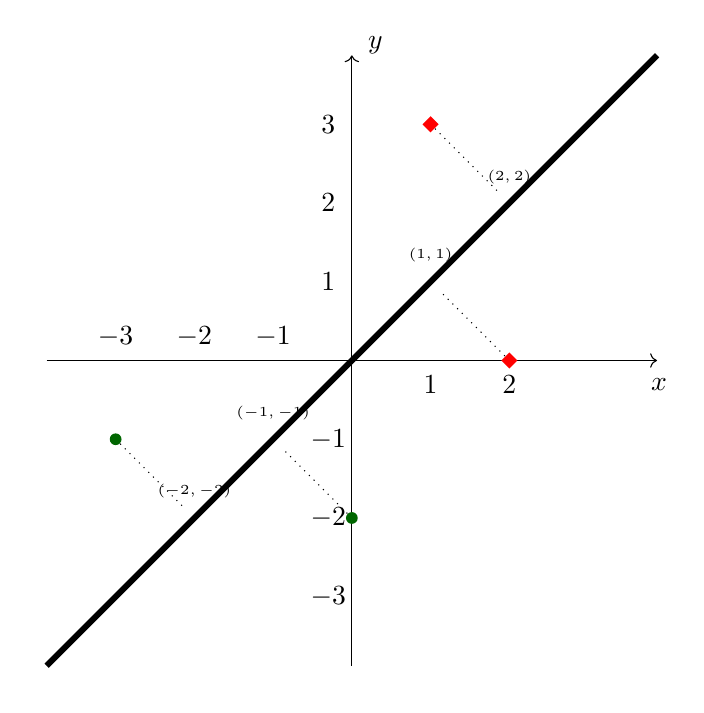
\begin{tikzpicture}
					\node (origin) at (0, 0) {};
					\node (top) at ($(origin) + (0, 4)$) {};
					\node (bottom) at ($(origin) + (0, -4)$) {};
					\node (left) at ($(origin) + (-4, 0)$) {};
					\node (right) at ($(origin) + (4, 0)$) {};
					\draw [->] (bottom) -- (top);
					\draw [->] (left) -- (right);
			
					\node at (-4, -4) (leftendpoint) {};
					\node at (4, 4) (rightendpoint) {};
					%\node at ($(origin) + (0.8, 1.3)$) {$y=\alpha x$};
					\node at ($(origin) + (3.9, -0.3)$) {$x$};
					\node at ($(origin) + (0.3, 4.0)$) {$y$};
			
					\draw[line width=0.75mm] (leftendpoint) -- (rightendpoint);
			
					\node[circle, fill=black!60!green, inner sep=1.5pt] at ($({-3/1.0}, {-1/1.0})$) (dp1) {};
					\node[circle, fill=black!60!green, inner sep=1.5pt] at ($({0/1.0}, {-2/1.0})$) (dp2) {};
					\node[diamond, fill=red, inner sep=1.5pt] at ($({2/1.0}, {0/1.0})$) (dp3) {};
					\node[diamond, fill=red, inner sep=1.5pt] at ($({1/1.0}, {3/1.0})$) (dp4) {};
					

					\node[label= {\tiny $\left( -2, -2\right)$}] at (-2, -2) (r1) {};
					\node[label= {\tiny $\left( -1, -1\right)$}] at (-1, -1) (r2) {};
					\node[label= {\tiny $\left( 1, 1\right)$}] at (1, 1) (r3) {};
					\node[label= {\tiny $\left( 2, 2\right)$}] at (2, 2) (r4) {};

					\draw[dotted] (dp1) -- (r1);
					\draw[dotted] (dp2) -- (r2);
					\draw[dotted] (dp3) -- (r3);
					\draw[dotted] (dp4) -- (r4);
			
					\node at ($({1/1.0}, 0.1)$) (dp1x) {};
					\node at ($(-0.1, {-2/1.0})$) (dp1y) {};
					\node at ($({1/1.0}, -0.3)$) {$1$};
					\node at ($(-0.3, {-2/1.0})$) {$-2$};
					%\draw[dotted] (dp1) -- (dp1x);
					%\draw[dotted] (dp1) -- (dp1y);
			
					\node at ($({2/1.0}, -0.1)$) (dp2x) {};
					\node at ($(-0.1, {3/1.0})$) (dp2y) {};
					\node at ($({2/1.0}, -0.3)$) {$2$};
					\node at ($(-0.3, {1/1.0})$) {$1$};
					\node at ($(-0.3, {2/1.0})$) {$2$};
					\node at ($(-0.3, {3/1.0})$) {$3$};
					%\draw[dotted] (dp2) -- (dp2x);
					%\draw[dotted] (dp2) -- (dp2y);
			
					\node at ($({-3/1.0}, 0.1)$) (dp3x) {};
					\node at ($(0.1, {-1/1.0})$) (dp3y) {};
					\node at ($({-3/1.0}, 0.3)$) {$-3$};
					\node at ($({-2/1.0}, 0.3)$) {$-2$};
					\node at ($({-1/1.0}, 0.3)$) {$-1$};
					\node at ($(-0.3, {-3/1.0} )$) {$-3$};
					\node at ($(-0.3, {-1/1.0} )$) {$-1$};
					%\draw[dotted] (dp3) -- (dp3x);
					%\draw[dotted] (dp3) -- (dp3y);
			
			
					\node[inner sep=0pt] at ($(leftendpoint)!(dp1)!(rightendpoint)$) (pdp1) {};
					\node[inner sep=0pt] at ($(leftendpoint)!(dp2)!(rightendpoint)$) (pdp2) {};
					\node[inner sep=0pt] at ($(leftendpoint)!(dp3)!(rightendpoint)$) (pdp3) {};
			
					%\draw[red] (dp1) -- (pdp1);
					%\draw[red] (dp2) -- (pdp2);
					%\draw[red] (dp3) -- (pdp3);
				\end{tikzpicture}
\end{Described}
				\caption{Plot of Transactions in 2-D}
			\end{figure}
		}


\end{enumerate}

  \newpage
  \qns{Diode System ID (Adapted from EECS 16B Fall 2023 Final)}

    \textbf{Note: This problem does not require knowledge of circuits or diodes.}
    
    Suppose that we want to characterize a diode $D_1$ with parasitic resistance $R_p$, represented by the following model:
    \begin{figure}[H]
        \begin{center}
            \begin{Described}{Voltage source V sub B drives from ground up to the top node, where diode D1 carries current I D to the right with voltage V D across it, in series with resistor R sub p returning to ground.}
\begin{circuitikz}
                \draw (0, 2) to [V, l_=$V_B$] (0, 0) node[ground]{}
                (0, 2) to [Do, l=$D_1$, i=$I_D$, v=$V_D$] (3, 2) to [R, l=$R_p$] (5, 2) node[ground]{}
                ;
            \end{circuitikz}
\end{Described}
        \end{center}
    \end{figure}
    The current through the diode (forward-biased) is modeled as
    \begin{equation}
        I_D = I_0\e^{\frac{V_D}{V_T}}
    \end{equation}
    where $V_D$ is the voltage across the diode (as shown in the diagram), $I_0$ is a parameter associated with the diode, and $V_T$ is the thermal voltage, a temperature dependent variable.
    
    With some analysis, the system equation can be simplified to:
    \begin{equation}
        I_D = I_0 \e^{\frac{V_B - I_D R_p}{V_T}}
    \end{equation}
    To collect data, we will vary the temperature to vary $V_T$ and measure the current $I_D$ through the diode.
    
        \begin{enumerate}

            \qitem    Use the provided system equation to show that
                \begin{equation}
                    I_D R_p - V_T \ln(I_0) = V_B - V_T \ln(I_D)
                \end{equation}
                    is a valid equation to represent the system.
                \begin{hint}
                    Use the logarithm identity $\ln(\frac{a}{b}) = \ln(a) - \ln(b)$.
                \end{hint}
            
    
            \ans{
                \begin{align}
                    I_D &= I_0 \e^{\frac{V_B - I_D R_p}{V_T}} \\
                    V_T\ln(\frac{I_D}{I_0}) &= V_B - I_D R_p \\
                    V_T\ln(I_D) - V_T\ln(I_0) &= V_B - I_D R_p \\
                    I_D R_p - V_T \ln(I_0) &= V_B - V_T \ln(I_D)
                \end{align}
            }
    
            % \begin{problempart}{4}{System ID}{0}{0}
            %     Suppose we use $V_B = 1 \mathrm{V}$ and collect the following data points:
            %     \begin{itemize}
            %         \item For $V_T = 0.025 \mathrm{V}$, $I_D = 0.0185 \mathrm{A}$.
            %         \item For $V_T = 0.05 \mathrm{V}$, $I_D = 0.0172 \mathrm{A}$.
            %         \item For $V_T = 0.0125 \mathrm{V}$, $I_D = 0.0193 \mathrm{A}$.
            %     \end{itemize}
            %     \textbf{Find the matrix $D$ and vector $\vec{s}$ to set up a least-squares problem $D\vec{p} \approx \vec{s}$ where $\vec{p} = \begin{bmatrix} \ln(I_0) \\ R_p \end{bmatrix}$.}
    
            %     You do not have to simplify the elements $D$ and $\vec{s}$, but the elements should be numerical values, not in terms of variables.
            % \end{problempart}
    
            % \begin{solution}{4in}
            %     Each data point can be used with the provided system equation from the first part to create a system of linear equations with the unknowns being $\ln(I_0)$ and $R_p$ (remember that the problem provides that $V_B = 1 \mathrm{V}$):
            %     \begin{itemize}
            %         \item $-0.025\ln(I_0) + 0.0185R_p = 1 - 0.025\ln(0.0185)$
            %         \item $-0.05\ln(I_0) + 0.0172R_p = 1 - 0.05\ln(0.0172)$
            %         \item $-0.0125\ln(I_0) + 0.0193R_p = 1 - 0.0125\ln(0.0193)$
            %     \end{itemize}
            %     The matrix form of this system is:
            %     \begin{equation}
            %         \begin{bmatrix} -0.025 & 0.0185 \\ -0.05 & 0.0172 \\ -0.0125 & 0.0193 \end{bmatrix} \begin{bmatrix} \ln(I_0) \\ R_p \end{bmatrix} = \begin{bmatrix} 1 - 0.025\ln(0.0185) \\ 1 - 0.05\ln(0.0172) \\ 1 - 0.0125\ln(0.0193) \end{bmatrix}
            %     \end{equation}
            %     Thus, for the least-squares problem, $D = \begin{bmatrix} -0.025 & 0.0185 \\ -0.05 & 0.0172 \\ -0.0125 & 0.0193 \end{bmatrix}$ and $\vec{s} = \begin{bmatrix} 1 - 0.025\ln(0.0185) \\ 1 - 0.05\ln(0.0172) \\ 1 - 0.0125\ln(0.0193) \end{bmatrix}$
            % \end{solution}
    
            \vspace{5cm}
            
            \qitem    Suppose we use $V_B = v_B$ and collect the following data points:
                \begin{itemize}
                    \item For $V_T = v_{T1}$, $I_D = i_{D1}$.
                    \item For $V_T = v_{T2}$, $I_D = i_{D2}$.
                    \item For $V_T = v_{T3}$, $I_D = i_{D3}$.
                \end{itemize}
                Find the matrix $\textbf{A}$ and vector $\vec{x}$ to set up a least-squares problem $\textbf{A} \vec{x} \approx \vec{b}$ where $\vec{x} = \begin{bmatrix} \ln(I_0) \\ R_p \end{bmatrix}$
    
            \ans{
                Each data point can be used with the provided system equation from the first part to create a system of linear equations with the unknowns being $\ln(I_0)$ and $R_p$ (remember that the problem provides that $V_B = v_B$):
                \begin{itemize}
                    \item $-v_{T1}\ln(I_0) + i_{D1}R_p = v_B - v_{T1}\ln(i_{D1})$
                    \item $-v_{T2}\ln(I_0) + i_{D2}R_p = v_B - v_{T2}\ln(i_{D2})$
                    \item $-v_{T3}\ln(I_0) + i_{D3}R_p = v_B - v_{T3}\ln(i_{D3})$
                \end{itemize}
                The matrix form of this system is:
                \begin{equation}
                    \begin{bmatrix} -v_{T1} & i_{D1} \\ -v_{T2} & i_{D2} \\ -v_{T3} & i_{D3} \end{bmatrix} \begin{bmatrix} \ln(I_0) \\ R_p \end{bmatrix} = \begin{bmatrix} v_B - v_{T1}\ln(i_{D1}) \\ v_B - v_{T2}\ln(i_{D2}) \\ v_B - v_{T3}\ln(i_{D3}) \end{bmatrix}
                \end{equation}
                Thus, for the least-squares problem, $\textbf{A} = \begin{bmatrix} -v_{T1} & i_{D1} \\ -v_{T2} & i_{D2} \\ -v_{T3} & i_{D3} \end{bmatrix}$ and $\vec{b} = \begin{bmatrix} v_B - v_{T1}\ln(i_{D1}) \\ v_B - v_{T2}\ln(i_{D2}) \\ v_B - v_{T3}\ln(i_{D3}) \end{bmatrix}$
            }
            
            \vspace{5cm}
            
            \qitem    Explain how you would use the least-squares system from the previous part to find model parameters $I_0$ and $R_p$. You do not need to use actual values for this part; you explanation can just use $\textbf{A}$ and $\vec{b}$ as known variables to show what calculations you would do to find $I_0$ and $R_p$.
            
    
            \ans{
                We would first find the optimal parameter $\hat{\vec{x}}$ with the least squares formula:
                \begin{equation}
                    \hat{\vec{x}} = (\textbf{A}^\top \textbf{A})^{-1} \textbf{A}^{\top} \vec{b}
                \end{equation}
                The elements of $\hat{\vec{x}}$ represent optimal values for $\ln(I_0)$ and $R_p$ so we set the elements of $\hat{\vec{x}}$ equal to those parameters for our model:
                \begin{align}
                    \hat{x}_{v_B} = \ln(I_0) &\rightarrow I_0 = \e^{\hat{x}_1} \\
                    \hat{x}_2 = R_p &\rightarrow R_p = \hat{x}_2
                \end{align}
                Thus, we have found parameter values for $I_0$ and $R_p$ from the least-squares system.
            }
    
        \end{enumerate}

\end{qunlist}

\end{document}
"
%   pdflatex "\PassOptionsToClass{prob}{latexally-assignment}% Demonstration built from REAL EECS 16A questionBank material, not from
% invented figures. Four question files were copied verbatim out of the corpus
% into corpus/ below, and `latexally apply` wrapped each figure in Described
% with a hand-written description. Nothing else in them was touched.
%
%   corpus/questionBank/sec/13/q_polynomial_fir_convolution.tex   1 figure
%   corpus/questionBank/sec/13/q_freq_resp_dag_diagram.tex        2 figures
%   corpus/sp26/dis/13A/questions/q_pca.tex                       4 figures
%   corpus/sp26/dis/13A/questions/q_diode_ls.tex                  1 figure
%
% Build both variants from this ONE source; build.sh supplies the class option:
%   pdflatex "\PassOptionsToClass{sol}{latexally-assignment}% Demonstration built from REAL EECS 16A questionBank material, not from
% invented figures. Four question files were copied verbatim out of the corpus
% into corpus/ below, and `latexally apply` wrapped each figure in Described
% with a hand-written description. Nothing else in them was touched.
%
%   corpus/questionBank/sec/13/q_polynomial_fir_convolution.tex   1 figure
%   corpus/questionBank/sec/13/q_freq_resp_dag_diagram.tex        2 figures
%   corpus/sp26/dis/13A/questions/q_pca.tex                       4 figures
%   corpus/sp26/dis/13A/questions/q_diode_ls.tex                  1 figure
%
% Build both variants from this ONE source; build.sh supplies the class option:
%   pdflatex "\PassOptionsToClass{sol}{latexally-assignment}% Demonstration built from REAL EECS 16A questionBank material, not from
% invented figures. Four question files were copied verbatim out of the corpus
% into corpus/ below, and `latexally apply` wrapped each figure in Described
% with a hand-written description. Nothing else in them was touched.
%
%   corpus/questionBank/sec/13/q_polynomial_fir_convolution.tex   1 figure
%   corpus/questionBank/sec/13/q_freq_resp_dag_diagram.tex        2 figures
%   corpus/sp26/dis/13A/questions/q_pca.tex                       4 figures
%   corpus/sp26/dis/13A/questions/q_diode_ls.tex                  1 figure
%
% Build both variants from this ONE source; build.sh supplies the class option:
%   pdflatex "\PassOptionsToClass{sol}{latexally-assignment}\input{demo-questionbank}"
%   pdflatex "\PassOptionsToClass{prob}{latexally-assignment}\input{demo-questionbank}"

\DocumentMetadata{
  lang       = en-US,
  pdfversion = 2.0,
  testphase  = {phase-III,math,table,graphic,firstaid},
}
\documentclass{latexally-assignment}

\usepackage{amsmath,amssymb}
\usepackage{float}
\usepackage{tikz}
\usetikzlibrary{calc,shapes.geometric,positioning}
\usepackage[american]{circuitikz}

% The corpus macros these four files use, reproduced from questionBank/ee16.sty
% and questionBank/sp26/sp26.sty so the demo does not need the whole course
% preamble chain. Same meanings, nothing more.
\providecommand{\bmqty}[1]{\begin{bmatrix}#1\end{bmatrix}}
\providecommand{\e}{\mathop{\mathrm{e}}\nolimits}
\providecommand{\wt}[1]{\widetilde{#1}}
\NewDocumentEnvironment{hint}{+b}{\itshape (HINT: #1)}{}

\setcoursenumber{EECS 16A}
\setcoursename{Designing Information Devices and Systems I}
\setsemester{Spring 2026}

\begin{document}

\def\title{Described figures from the question bank}
\maketitle

\vspace{0.5em}
Every figure below carries a description in the PDF structure tree. A screen
reader announces "graphic" and then that description; it never reaches the
drawing underneath. Hovering shows nothing --- \texttt{/Alt} is not a tooltip.

\begin{qunlist}

  \input{corpus/questionBank/sec/13/q_polynomial_fir_convolution.tex}
  \newpage
  \input{corpus/questionBank/sec/13/q_freq_resp_dag_diagram.tex}
  \newpage
  \input{corpus/sp26/dis/13A/questions/q_pca.tex}
  \newpage
  \input{corpus/sp26/dis/13A/questions/q_diode_ls.tex}

\end{qunlist}

\end{document}
"
%   pdflatex "\PassOptionsToClass{prob}{latexally-assignment}% Demonstration built from REAL EECS 16A questionBank material, not from
% invented figures. Four question files were copied verbatim out of the corpus
% into corpus/ below, and `latexally apply` wrapped each figure in Described
% with a hand-written description. Nothing else in them was touched.
%
%   corpus/questionBank/sec/13/q_polynomial_fir_convolution.tex   1 figure
%   corpus/questionBank/sec/13/q_freq_resp_dag_diagram.tex        2 figures
%   corpus/sp26/dis/13A/questions/q_pca.tex                       4 figures
%   corpus/sp26/dis/13A/questions/q_diode_ls.tex                  1 figure
%
% Build both variants from this ONE source; build.sh supplies the class option:
%   pdflatex "\PassOptionsToClass{sol}{latexally-assignment}\input{demo-questionbank}"
%   pdflatex "\PassOptionsToClass{prob}{latexally-assignment}\input{demo-questionbank}"

\DocumentMetadata{
  lang       = en-US,
  pdfversion = 2.0,
  testphase  = {phase-III,math,table,graphic,firstaid},
}
\documentclass{latexally-assignment}

\usepackage{amsmath,amssymb}
\usepackage{float}
\usepackage{tikz}
\usetikzlibrary{calc,shapes.geometric,positioning}
\usepackage[american]{circuitikz}

% The corpus macros these four files use, reproduced from questionBank/ee16.sty
% and questionBank/sp26/sp26.sty so the demo does not need the whole course
% preamble chain. Same meanings, nothing more.
\providecommand{\bmqty}[1]{\begin{bmatrix}#1\end{bmatrix}}
\providecommand{\e}{\mathop{\mathrm{e}}\nolimits}
\providecommand{\wt}[1]{\widetilde{#1}}
\NewDocumentEnvironment{hint}{+b}{\itshape (HINT: #1)}{}

\setcoursenumber{EECS 16A}
\setcoursename{Designing Information Devices and Systems I}
\setsemester{Spring 2026}

\begin{document}

\def\title{Described figures from the question bank}
\maketitle

\vspace{0.5em}
Every figure below carries a description in the PDF structure tree. A screen
reader announces "graphic" and then that description; it never reaches the
drawing underneath. Hovering shows nothing --- \texttt{/Alt} is not a tooltip.

\begin{qunlist}

  \input{corpus/questionBank/sec/13/q_polynomial_fir_convolution.tex}
  \newpage
  \input{corpus/questionBank/sec/13/q_freq_resp_dag_diagram.tex}
  \newpage
  \input{corpus/sp26/dis/13A/questions/q_pca.tex}
  \newpage
  \input{corpus/sp26/dis/13A/questions/q_diode_ls.tex}

\end{qunlist}

\end{document}
"

\DocumentMetadata{
  lang       = en-US,
  pdfversion = 2.0,
  testphase  = {phase-III,math,table,graphic,firstaid},
}
\documentclass{latexally-assignment}

\usepackage{amsmath,amssymb}
\usepackage{float}
\usepackage{tikz}
\usetikzlibrary{calc,shapes.geometric,positioning}
\usepackage[american]{circuitikz}

% The corpus macros these four files use, reproduced from questionBank/ee16.sty
% and questionBank/sp26/sp26.sty so the demo does not need the whole course
% preamble chain. Same meanings, nothing more.
\providecommand{\bmqty}[1]{\begin{bmatrix}#1\end{bmatrix}}
\providecommand{\e}{\mathop{\mathrm{e}}\nolimits}
\providecommand{\wt}[1]{\widetilde{#1}}
\NewDocumentEnvironment{hint}{+b}{\itshape (HINT: #1)}{}

\setcoursenumber{EECS 16A}
\setcoursename{Designing Information Devices and Systems I}
\setsemester{Spring 2026}

\begin{document}

\def\title{Described figures from the question bank}
\maketitle

\vspace{0.5em}
Every figure below carries a description in the PDF structure tree. A screen
reader announces "graphic" and then that description; it never reaches the
drawing underneath. Hovering shows nothing --- \texttt{/Alt} is not a tooltip.

\begin{qunlist}

  \qns{Polynomial Multiplication and Discrete-Time Convolution [Adapted from EE 120]}
% Adapted and extended by Ken Zheng for EECS 16A Fall 2025 Discussion

The impulse response of a real, discrete-time FIR filter $\mathsf{A}$ is described by  
$$a[n]=a_0 \delta[n]+a_1 \delta[n-1]+\cdots + a_N \delta[n-N], \quad \text{where } N\in \{1,2,3,\ldots\}.$$

\begin{enumerate}[(a)]
\item Show that the frequency response $A(\omega)$ of the filter is a polynomial, in terms of $e^{-i\omega}$, whose coefficients have a simple relationship with the impulse response values $a_0,\ldots,a_N$.

\ans{

    Substituting \(a[n]\) into the frequency response formula we see that:
    \begin{equation*}
        A(w) = \sum_{n=-\infty}^{\infty} a[n]e^{-iwn}
    \end{equation*}
    As $a[n] = 0$ outside the range of $n = 0$ to $n = N$ ,
    \begin{equation*}
        A(w) = a_0 e^{-iw\cdot 0} + a_1 e^{-iw\cdot 1} + \ldots + a_N e^{-iw\cdot N}
    \end{equation*}
    \begin{equation*}
        = a_0 + a_1 e^{-iw} + \ldots + a_N e^{-iwN}
    \end{equation*}
}
\item Suppose the filter $\mathsf{A}$ is placed in a cascade (series) interconnection with another discrete-time FIR filter $\mathsf{B}$ whose impulse response is described by  
$$b[n]=b_0 \delta[n]+b_1 \delta[n-1]+\cdots + b_M \delta[n-M],\quad \text{where } M\in \{1,2,3,\ldots\}.$$

The cascade structure, which we call $\mathsf{C}$, is shown in the figure below.
\vspace{4pt}

\centerline{
    \begin{Described}{Block diagram: input x enters block A, whose output feeds block B, and block B's output is y. An outer box enclosing both blocks is labelled C.}
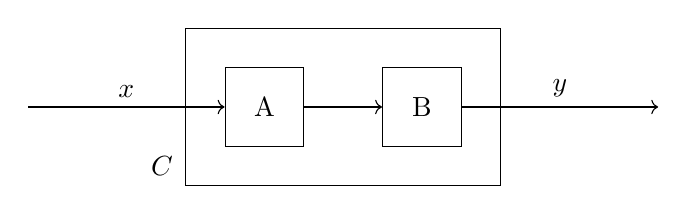
\begin{tikzpicture}
        % Define nodes for blocks A and B
        \node[draw, rectangle, minimum width=1cm, minimum height=1cm] (A) at (0,0) {A};
        \node[draw, rectangle, minimum width=1cm, minimum height=1cm] (B) at (2,0) {B};
        
        % Draw the outer rectangle
        \draw (-1, 1) rectangle (3, -1);
        
        % Draw arrows and labels
        \draw[->] (-3, 0) -- (A.west) node[midway,above] {$x$};
        \draw[->] (A.east) -- (B.west);
        \draw[->] (B.east) -- (5, 0) node[midway,above] {$y$};
        
        % Label C 
        \node at (-1.3, -0.5) [below] {$C$};
    \end{tikzpicture}
\end{Described}
}
Let $c$ denote the impulse response of the cascade interconnection.

\begin{enumerate}[(i)]
\item Express $c$ in terms of $a$ and $b$.
    
\ans{

        The impulse response \(c\) of the cascade interconnection is given by 
        \begin{equation*}
            c[n] = (a * b)[n] = \sum_{k=-\infty}^{\infty} a[k]\,b[n-k]
        \end{equation*}
         Substituting \(n = 0\):
        \begin{equation*}
            c_0 = a_0 b_0
        \end{equation*}
        \(n = 1\):
        \begin{equation*}
            c_1 = a_0 b_1 + a_1 b_0 
        \end{equation*}
        \(n = 2\):
        \begin{equation*}
            c_2 = a_0 b_2 + a_1 b_1 + a_2 b_0
        \end{equation*}
        And so on...
    
        Thus, we can write:
        \begin{equation*}
            c_n = \sum_{k=\max(0,n-M)}^{\min(n, N)} a_k b_{n-k}
        \end{equation*}
        \null\hfill for \(n = 0, 1, \ldots, N + M\)
        
        where we found the bounds of summation from the two conditions that ensure we are indexing \(a[n]\) and \(b[n]\) without exceeding the bounds of their signal.
        $$ 0 \leq k \leq N \Longrightarrow k \leq N \quad \text{and} \quad k \geq 0 $$
        $$ 0 \leq n - k \leq M \Longrightarrow k \leq n \quad \text{and} \quad k \geq n - M $$
        and so
        $$ k \leq \min(n, N) \quad \text{and} \quad k \geq \max(0, n-M) $$

        Lastly, 
         \begin{equation*}
            c[n] = c_0\delta[n] + c_1 \delta[n - 1] + ... + c_{N + M} \delta[n - ( N + M)]
        \end{equation*}
        
    }

\item Consider two polynomials $A(z)$ and $B(z)$ described as follows:
    $$
    A(z) = a_0 +a_1 z + \cdots + a_N z^N \quad \quad \quad B(z) = b_0 +b_1 z + \cdots + b_M z^M \, ,
    $$
    where $M$ and $N$ and positive integers.
    Let $C(z)=A(z)\, B(z)$, where $$ C(z) = c_0 +c_1 z + \cdots + c_{N+M} z^{N+M}.$$  Show that multiplying polynomials is tantamount to convolving their coefficients; in particular, explain how $c_n=(a*b)_n=\displaystyle\sum_m a_m b_{n-m}$, where $n={0,1,\ldots, N+M}$.
    
    \ans{
    \begin{equation*}
        C(z) = (a_0 +a_1 z + \cdots + a_N z^N) (b_0 +b_1 z + \cdots + b_M z^M)
    \end{equation*}
    \begin{equation*}
        C(z) = a_0 b_0 + (a_0 b_1 + a_1 b_0) z + (a_0 b_2 + a_1 b_1 + a_2 b_0) z^2 + ...
    \end{equation*}
    As you can see, each coefficient of \(z^n\) is the sum of all products of \(a_i\) and \(b_j\) where \(i + j = n\):
    \begin{equation*}
        c_n =  \sum_{m=\max(0,n-M)}^{\min(n, N)} a_m b_{n-m}
    \end{equation*}
    \null\hfill for \(n = 0, 1, 2, ..., N + M\)

    Just like the definition of convolution!
    }

\end{enumerate}
\end{enumerate}
  \newpage
  \qns{Frequency Response from a DAG Block Diagram [Adapted from EE 120]}
% Adapted by Ken Zheng for EECS 16A Fall 2025 Discussion

    Consider a DT LTI system with input $x[n]$ and output $y[n]$ that is implemented by the following block diagram:
    \begin{figure}[h!]
      \centering
      \begin{Described}{Block diagram: input x of n enters a summing junction whose output is y of n. That output is tapped, passed through a delay block D and then a gain of minus 0.5, and fed back into the summing junction.}
\begin{circuitikz}
          \node (x) at (0, 0) {$x[n]$};
          \node[circle, draw] (sum) at (2, 0) {$+$};
          % FIXME: find a better way to draw the triangle
          % \node[triangleblock, shape border rotate=90, inner sep=-1mm] (gain) at (3, -1.5) {$-0.5$};
          % \node at (3, -1.5) {$-0.5$};
          \node[draw, inner sep=5pt] (delay) at (6, -1.5) {$D$};
          \node (y) at (9, 0) {$y[n]$};
          \draw[->] (x.east) -- (sum.west);
          \draw[->] (sum.east) -- (y.west);
          \draw[->] (7.5, 0) -- (7.5, -1.5) -- (delay.east);
          % \draw[-, thick] (delay.west) -- (gain.east);
          % \draw[->, thick] (gain.west) -- (2, -1.5) -- (sum.south);
          \draw[->] (delay.west) to [amp, t=$-0.5$, blocks/scale=1.5] (2, -1.5) to (sum.south);
      \end{circuitikz}
\end{Described}
  \end{figure}
\begin{enumerate}
        \item Find the LCCDE that describes this system. 
        
        \ans{
            The difference equation describing this system is
              \begin{equation*}
                y[n] = x[n] - 0.5y[n-1]
              \end{equation*}
        }

        \item Find the frequency response $H(\omega)$ of this system. 
            
        \ans{
            Using the eigenfunction property by setting $x[n] = e^{i\omega n}$ and $y[n] = H(\omega) e^{i\omega n}$,
            \begin{align*}
            H(\omega) e^{i\omega n} &= e^{i\omega n} - 0.5 H(\omega) e^{i\omega (n-1)} \\
            &= e^{i\omega n} - 0.5 H(\omega) e^{-i\omega}e^{i\omega n} \\
            \left(1 + 0.5 e^{-i\omega}\right) e^{i\omega n} H(\omega) &= e^{i\omega n} \\
            H(\omega) &= \frac{e^{i\omega n}}{\left(1 + 0.5 e^{-i\omega}\right)e^{i\omega n}} \\
                &= \frac{1}{1 + 0.5 e^{-i\omega}}
            \end{align*} 
        } 

        \vspace{4cm}

        \item Is this a high pass or low pass filter?
        
        \ans{
            We can think about this in two ways:
            
            \textbf{1. Geometric Approach:}

            Recall from part (b) that the frequency response can be written as:
            \[
            H(\omega) = \frac{1}{1 + 0.5 e^{-i\omega}} = \frac{e^{i\omega}}{e^{i\omega} - (-0.5)}
            \]
            The magnitude is therefore:
            \[
            |H(\omega)| = \frac{1}{|e^{i\omega} - (-0.5)|}
            \]
            This represents the reciprocal of the distance from the point $e^{i\omega}$ on the unit circle to the point located at $-0.5$ on the real axis:

            \begin{center}
            \begin{Described}{Complex plane with real and imaginary axes and the unit circle centred at the origin. A point is marked at minus 0.5 on the real axis, with an arrow from it to the point e to the i omega on the circle.}
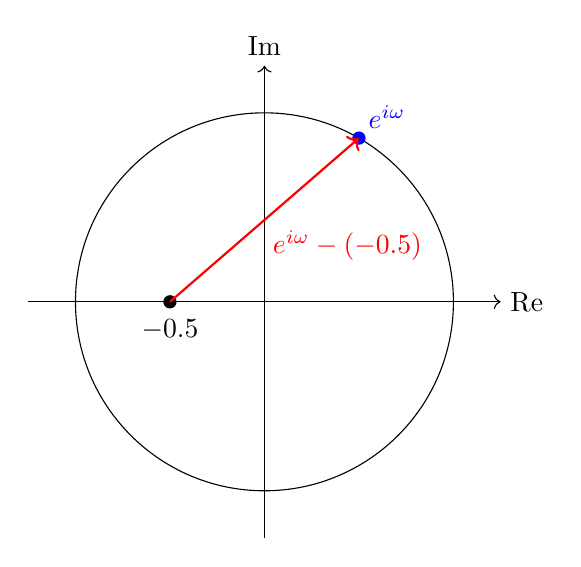
\begin{tikzpicture}[scale=1.2]
                % Axes
                \draw[->] (-2.5,0) -- (2.5,0) node[right] {$\operatorname{Re}$};
                \draw[->] (0,-2.5) -- (0,2.5) node[above] {$\operatorname{Im}$};

                % Unit circle
                \draw (0,0) circle (2);

                % Pole at -0.5
                \fill[black] (-1,0) circle (2pt) node[below left] {};
                \node[black] at (-1,-0.3) {$-0.5$};

                % Point on unit circle at angle ω
                \coordinate (P) at (60:2);
                \fill[blue] (P) circle (2pt) node[above right] {$e^{i\omega}$};

                % Vector from pole to point on circle
                % \draw[->, thick, red] (-1,0) -- (P);
                \draw[->, thick, red] (-1,0) -- (P) node[midway, below] {$\qquad\qquad\qquad e^{i \omega} - (-0.5)$};  % Label added here


                % Labels
                \node at (1.8,1.8) {};
            \end{tikzpicture}
\end{Described}
            \end{center}

            Key observations:
            \begin{itemize}
                \item When $\omega = 0$, $e^{i\omega} = 1$. The distance from $1$ to $-0.5$ is $1.5$, so $|H(0)| = 1/1.5 \approx 0.667$.
                \item When $\omega = \pi$, $e^{i\omega} = -1$. The distance from $-1$ to $-0.5$ is $0.5$, so $|H(\pi)| = 1/0.5 = 2$.
                \item As $\omega$ moves from $0$ to $\pi$, the point $e^{i\omega}$ travels along the upper half of the unit circle from $(1,0)$ to $(-1,0)$. 
                The distance to the point at $-0.5$ decreases monotonically, so $|H(\omega)|$ increases. Thus, we have a high-pass filter!\\
            \end{itemize}

            
            \textbf{2. Algebraic Approach:}
            
            To determine the filter type, we simplify the magnitude of the frequency response first:

            \[
            |H(\omega)| = \frac{1}{\sqrt{(1 + 0.5\cos\omega)^2 + (0.5\sin\omega)^2}}
            \]


            Expanding \( (1 + 0.5\cos\omega)^2 \) and \( (0.5\sin\omega)^2 \):
            \[
            (1 + 0.5\cos\omega)^2 = 1^2 + 2(1)(0.5\cos\omega) + (0.5\cos\omega)^2 = 1 + \cos\omega + 0.25\cos^2\omega
            \]
            \[
            (0.5\sin\omega)^2 = 0.25\sin^2\omega
            \]


            Add the two results in the square root:
            \[
            (1 + 0.5\cos\omega)^2 + (0.5\sin\omega)^2 = \left[1 + \cos\omega + 0.25\cos^2\omega\right] + \left[0.25\sin^2\omega\right]
            \]
            \[
            = 1 + \cos\omega + 0.25\left(\cos^2\omega + \sin^2\omega\right)
            \]
            \[
            = 1 + \cos\omega + 0.25(1) = 1 + \cos\omega + 0.25 = 1.25 + \cos\omega
            \]


            Substitute back into \( |H(\omega)| \):
            \[
            |H(\omega)| = \frac{1}{\sqrt{1.25 + \cos\omega}}
            \]
                        
            Now we analyze the magnitude at key frequencies:
            
            Low frequency (\( \omega = 0 \)): 
                \[
                |H(0)| =  \frac{1}{\sqrt{1.25 + \cos0}} = \frac{1}{1.5} \approx 0.667 \quad (\text{attenuated})
                \]
            High frequency (\( \omega = \pi \)): 
                \[
                |H(\pi)| =  \frac{1}{\sqrt{1.25 + \cos\pi}} = 2 \quad (\text{passed})
                \]

            We can see that, again, the filter attenuates low frequencies and passes high frequencies, so it is a high-pass filter!\\

            Both geometrically and algebraically, we conclude this is a \textbf{high-pass filter}. Nice!
        }
\end{enumerate}

  \newpage
  \qns{Using PCA to Detect Fraudulent Transactions (Adapted from EECS 16B Spring 2023 Final)}\\
	PCA has many different uses when applied to real-world data. One potential application is making classification of data much easier.
	
	Suppose we are given some data, where each datapoint represents a transaction. Each one is labeled either normal or fraudulent. We will utilize PCA to develop a useful classifier.

	We plot the data in two dimensions, where each dimension is some unspecified feature that will aid us in classifying the points:

	\begin{figure}[H]
        \centering
        \begin{Described}{Scatter plot on x and y axes running about minus 4 to 4, with four transactions marked: circles at (-3, -1) and (0, -2), and diamonds at (2, 0) and (1, 3).}
\begin{tikzpicture}
            \node (origin) at (0, 0) {};
            \node (top) at ($(origin) + (0, 4)$) {};
            \node (bottom) at ($(origin) + (0, -4)$) {};
            \node (left) at ($(origin) + (-4, 0)$) {};
            \node (right) at ($(origin) + (4, 0)$) {};
            \draw [->] (bottom) -- (top);
            \draw [->] (left) -- (right);
    
            \node at (-3, -2.2) (leftendpoint) {};
            \node at (3, 2.2) (rightendpoint) {};
            %\node at ($(origin) + (0.8, 1.3)$) {$y=\alpha x$};
            \node at ($(origin) + (3.9, -0.3)$) {$x$};
            \node at ($(origin) + (0.3, 4.0)$) {$y$};
    
            %\draw[line width=0.75mm] (leftendpoint) -- (rightendpoint);
    
            \node[circle, fill=black!60!green, inner sep=1.5pt] at ($({-3/1.0}, {-1/1.0})$) (dp1) {};
            \node[circle, fill=black!60!green, inner sep=1.5pt] at ($({0/1.0}, {-2/1.0})$) (dp2) {};
            \node[diamond, fill=red, inner sep=1.5pt] at ($({1/1.0}, {3/1.0})$) (dp3) {};
			\node[diamond, fill=red, inner sep=1.5pt] at ($({2/1.0}, {0/1.0})$) (dp4) {};
    
            \node at ($({1/1.0}, 0.1)$) (dp1x) {};
            \node at ($(-0.1, {-2/1.0})$) (dp1y) {};
            \node at ($({1/1.0}, 0.3)$) {$1$};
            \node at ($(-0.3, {-2/1.0})$) {$-2$};
            %\draw[dotted] (dp1) -- (dp1x);
            %\draw[dotted] (dp1) -- (dp1y);
    
            \node at ($({2/1.0}, -0.1)$) (dp2x) {};
            \node at ($(-0.1, {3/1.0})$) (dp2y) {};
            \node at ($({2/1.0}, -0.3)$) {$2$};
            \node at ($(-0.3, {3/1.0})$) {$3$};
            %\draw[dotted] (dp2) -- (dp2x);
            %\draw[dotted] (dp2) -- (dp2y);
    
            \node at ($({-3/1.0}, 0.1)$) (dp3x) {};
            \node at ($(0.1, {-1/1.0})$) (dp3y) {};
            \node at ($({-3/1.0}, 0.3)$) {$-3$};
            \node at ($(-0.3, {-1/1.0 -0.3} )$) {$-1$};
            %\draw[dotted] (dp3) -- (dp3x);
            %\draw[dotted] (dp3) -- (dp3y);
    
    
            \node[inner sep=0pt] at ($(leftendpoint)!(dp1)!(rightendpoint)$) (pdp1) {};
            \node[inner sep=0pt] at ($(leftendpoint)!(dp2)!(rightendpoint)$) (pdp2) {};
            \node[inner sep=0pt] at ($(leftendpoint)!(dp3)!(rightendpoint)$) (pdp3) {};
    
            %\draw[red] (dp1) -- (pdp1);
            %\draw[red] (dp2) -- (pdp2);
            %\draw[red] (dp3) -- (pdp3);
        \end{tikzpicture}
\end{Described}
        \caption{Plot of Transactions in 2-D}
	\end{figure}

	Thus, we have a total of 4 transactions, $\bmqty{-3 \\ -1}$ and $\bmqty{0 \\ -2}$ are normal, while $\bmqty{2 \\ 0}$ and $\bmqty{1 \\ 3}$ are fraudulent.
	\begin{enumerate}
		%Part A:
		
		\qitem Suppose we now construct a data matrix, where the \textit{data points are columns}. 

			\begin{equation}
				X = \bmqty{-3 & 0 & 2 & 1 \\ -1 & -2 & 0 & 3}
			\end{equation}

			Using this data matrix, \textbf{calculate its first principal component $\vec{u}_1$}.

			\begin{hint}
			\begin{enumerate}

				\item You may also make use of the fact that $XX^T$ is given by:
				\begin{align}
					XX^{\top} &= \bmqty{-3 & 0 & 2 & 1 \\ -1 & -2 & 0 & 3}\bmqty{-3 & 0 & 2 & 1 \\ -1 & -2 & 0 & 3}^{\top} \\
						&= \bmqty{14 & 6 \\ 6 & 14}
				\end{align}
				\item You may also make use of the characteristic polynomial of $XX^T$:
				\begin{equation}
					\lambda^2 - 28\lambda + 160 = (\lambda - 20)(\lambda - 8) = 0
				\end{equation}
			\end{enumerate}
			\end{hint}
			
			\begin{hint} Remember that your principal component should be of unit norm. \end{hint}

		\ans{
			% From PCA, we know that our first principal component of a matrix with column data is the first column vector of $U$ in the SVD of $X$. Thus, we use the SVD method of calculation (find the eigenvector corresponding to the largest eigenvalue of $XX^{\top}$ and normalize to yield $\vec{u}_1$).

			% \begin{align}
			% 	XX^{\top} &= \bmqty{-3 & 0 & 2 & 1 \\ -1 & -2 & 0 & 3}\bmqty{-3 & 0 & 2 & 1 \\ -1 & -2 & 0 & 3}^{\top} \\
			% 		 &= \bmqty{14 & 6 \\ 6 & 14}
			% \end{align}

			% From setting $\mathrm{det}(XX^{\top} - \lambda I) = 0$, we should find our characteristic polynomial to be 
			
			% \begin{equation}
			% 	\lambda^2 - 28\lambda + 160 = 0
			% \end{equation}

			Our eigenvalues are $\lambda_1 = 20$ and $\lambda_2 = 8$. Thus, the eigenvector corresponding to our largest eigenvalue $\lambda_1 = 20$ is $\vec{v}_1 = \bmqty{1 \\ 1}$ from inspection.
			
			Thus, our principal component vector is given as the normalized eigenvector: i.e. $\vec{u}_1 = \bmqty{\frac{1}{\sqrt{2}} \\ \frac{1}{\sqrt{2}}}$.
        }

		%Part B:
		
		\qitem	It's difficult to come up with a useful classifier in two dimensions. Let's use PCA dimensionality reduction to help.
			
			Using your answer in part (a), \textbf{project your two-dimensional data points onto one dimension. Express your answer as the vector $\vec{z} \in \mathbb{R}^{1 \times 4}$.}

		\ans{
			To project our 2-d data into 1-d, we project our data matrix onto the first principal component as follows:
			
			\begin{equation}
				\vec{z} = \vec{u}_1^{\top}X = \bmqty{\frac{1}{\sqrt{2}} \\ \frac{1}{\sqrt{2}}} \bmqty{-3 & 0 & 2 & 1 \\ -1 & -2 & 0 & 3} = \bmqty{-\frac{4}{\sqrt{2}} & -\frac{2}{\sqrt{2}} & \frac{2}{\sqrt{2}} & \frac{4}{\sqrt{2}}}
			\end{equation}
		}
		
		%Part C:
		
		\qitem	Now, plot each of these points, on the line below. Indicate the value and label (normal as circle and fraudulent as diamond) for each point.
			
			\textit{Note: your plot doesn't have to be to scale.}

			\begin{figure}[H]
				\centering
				\begin{Described}{Blank horizontal number line labelled z, with only the origin marked 0 and no points plotted.}
\begin{tikzpicture}
					\node (origin) at (0, 0) {|};
            		%\node (top) at ($(origin) + (0, 4)$) {};
            		%\node (bottom) at ($(origin) + (0, -4)$) {};
            		\node (left) at ($(origin) + (-4, 0)$) {};
            		\node (right) at ($(origin) + (4, 0)$) {};
					\node at ($(origin) + (3.9, -0.3)$) {$z$};
					\node at ($(origin) + (0, -0.3)$) {0};
            		%\draw [->] (bottom) -- (top);
            		\draw [<->] (left) -- (right);

				\end{tikzpicture}
\end{Described}
				\caption{Plot of Transactions in 1-D}
			\end{figure}

		\ans{
			\begin{figure}[H]
				\centering
				\begin{Described}{Number line labelled z with the origin marked 0 and four points: circles at minus four over root two and minus two over root two, diamonds at two over root two and four over root two.}
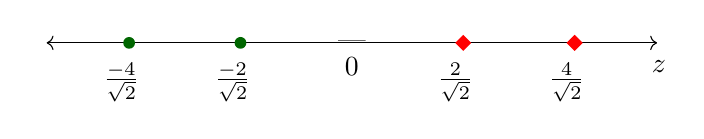
\begin{tikzpicture}
					\node (origin) at (0, 0) {|};
            		%\node (top) at ($(origin) + (0, 4)$) {};
            		%\node (bottom) at ($(origin) + (0, -4)$) {};
            		\node (left) at ($(origin) + (-4, 0)$) {};
            		\node (right) at ($(origin) + (4, 0)$) {};
					\node at ($(origin) + (3.9, -0.3)$) {$z$};
					\node at ($(origin) + (0, -0.3)$) {0};
            		%\draw [->] (bottom) -- (top);
            		\draw [<->] (left) -- (right);

					\node[circle, fill=black!60!green, inner sep=1.5pt] at ($(origin) + (-4/1.414, 0)$) (dp1) {};
					\node at ($(origin) + (-4/1.414 -0.1, -0.5)$) {$\frac{-4}{\sqrt{2}}$};
					\node[circle, fill=black!60!green, inner sep=1.5pt] at ($(origin) + (-2/1.414, 0)$) (dp1) {};
					\node at ($(origin) + (-2/1.414 -0.1, -0.5)$) {$\frac{-2}{\sqrt{2}}$};
					\node[diamond, fill=red, inner sep=1.5pt] at ($(origin) + (2/1.414, 0)$) (dp1) {};
					\node at ($(origin) + (2/1.414 -0.1, -0.5)$) {$\frac{2}{\sqrt{2}}$};
					\node[diamond, fill=red, inner sep=1.5pt] at ($(origin) + (4/1.414, 0)$) (dp1) {};
					\node at ($(origin) + (4/1.414 -0.1, -0.5)$) {$\frac{4}{\sqrt{2}}$};
				\end{tikzpicture}
\end{Described}
				\caption{Plot of Transactions in 1-D}
			\end{figure}
		}

		%Part D:
		
		\qitem	Suppose you are given some transaction datapoint, $\vec{x}_i$ and you project it to be one-dimensional, i.e. $z_i$. \textbf{Based on your plot from part (c), come up with an inequality in terms of $z_i$ to identify if that transaction is fraudulent.}
			
			\textit{Note: There can be more than one answer, but please only give one.}

		\ans{
			$\vec{z}_i > 0$ is a possible answer. In fact any answer in between $\vec{z}_i \geq -\frac{2}{\sqrt{2}}$ and $\vec{z}_i \geq \frac{2}{\sqrt{2}}$ is valid.
		}

		%Part E:
		
		\qitem	It can often be informative to compare our original data with its PCA reconstructions. \textbf{Using PCA, reconstruct $\vec{z}$ back into 2-D as the matrix $\wt{X} \in \mathbb{R}^{2 \times 4}$.}

		\ans{
			Using the reconstruction principle of PCA, we lift the 1D data back into 2 dimensions by doing the following:
			\begin{equation}
				\wt{X} = \vec{u}_1\vec{u}_1^{\top}X = \bmqty{-2 & -1 & 1 & 2 \\ -2 & -1 & 1 & 2}
			\end{equation}
		}

		%Part F:
		
		\qitem	Finally, we visualize our PCA reconstruction. \textbf{On the graph below, draw your first principal component direction (extend it as a solid line in both directions). Draw your reconstructioned points from $\wt{X}$, with dotted lines connecting them with the corresponding point in $X$. } You may draw on the plot on the next page.

			\begin{figure}[H]
				\centering
				\begin{Described}{Scatter plot on x and y axes running about minus 4 to 4, with four transactions marked: circles at (-3, -1) and (0, -2), and diamonds at (2, 0) and (1, 3).}
\begin{tikzpicture}
					\node (origin) at (0, 0) {};
					\node (top) at ($(origin) + (0, 4)$) {};
					\node (bottom) at ($(origin) + (0, -4)$) {};
					\node (left) at ($(origin) + (-4, 0)$) {};
					\node (right) at ($(origin) + (4, 0)$) {};
					\draw [->] (bottom) -- (top);
					\draw [->] (left) -- (right);
			
					\node at (-3, -2.2) (leftendpoint) {};
					\node at (3, 2.2) (rightendpoint) {};
					%\node at ($(origin) + (0.8, 1.3)$) {$y=\alpha x$};
					\node at ($(origin) + (3.9, -0.3)$) {$x$};
					\node at ($(origin) + (0.3, 4.0)$) {$y$};
			
					%\draw[line width=0.75mm] (leftendpoint) -- (rightendpoint);
			
					\node[circle, fill=black!60!green, inner sep=1.5pt] at ($({-3/1.0}, {-1/1.0})$) (dp1) {};
					\node[circle, fill=black!60!green, inner sep=1.5pt] at ($({0/1.0}, {-2/1.0})$) (dp2) {};
					\node[diamond, fill=red, inner sep=1.5pt] at ($({1/1.0}, {3/1.0})$) (dp3) {};
					\node[diamond, fill=red, inner sep=1.5pt] at ($({2/1.0}, {0/1.0})$) (dp4) {};
			
					\node at ($({1/1.0}, 0.1)$) (dp1x) {};
					\node at ($(-0.1, {-2/1.0})$) (dp1y) {};
					\node at ($({1/1.0}, 0.3)$) {$1$};
					\node at ($(-0.3, {-2/1.0})$) {$-2$};
					%\draw[dotted] (dp1) -- (dp1x);
					%\draw[dotted] (dp1) -- (dp1y);
			
					\node at ($({2/1.0}, -0.1)$) (dp2x) {};
					\node at ($(-0.1, {3/1.0})$) (dp2y) {};
					\node at ($({2/1.0}, -0.3)$) {$2$};
					\node at ($(-0.3, {3/1.0})$) {$3$};
					%\draw[dotted] (dp2) -- (dp2x);
					%\draw[dotted] (dp2) -- (dp2y);
			
					\node at ($({-3/1.0}, 0.1)$) (dp3x) {};
					\node at ($(0.1, {-1/1.0})$) (dp3y) {};
					\node at ($({-3/1.0}, 0.3)$) {$-3$};
					\node at ($(-0.3, {-1/1.0 -0.3} )$) {$-1$};
					%\draw[dotted] (dp3) -- (dp3x);
					%\draw[dotted] (dp3) -- (dp3y);
			
			
					\node[inner sep=0pt] at ($(leftendpoint)!(dp1)!(rightendpoint)$) (pdp1) {};
					\node[inner sep=0pt] at ($(leftendpoint)!(dp2)!(rightendpoint)$) (pdp2) {};
					\node[inner sep=0pt] at ($(leftendpoint)!(dp3)!(rightendpoint)$) (pdp3) {};
			
					%\draw[red] (dp1) -- (pdp1);
					%\draw[red] (dp2) -- (pdp2);
					%\draw[red] (dp3) -- (pdp3);
				\end{tikzpicture}
\end{Described}
				\caption{Plot of Transactions in 2-D}
			\end{figure}

		\ans{

			Using the answer from part (d), students should end up with the following graph:
			\begin{figure}[H]
				\centering
				\begin{Described}{The same four transactions, with a solid line through the origin along y = x and reconstructed points on it at (-2, -2), (-1, -1), (1, 1) and (2, 2), each joined to its original point by a dotted line.}
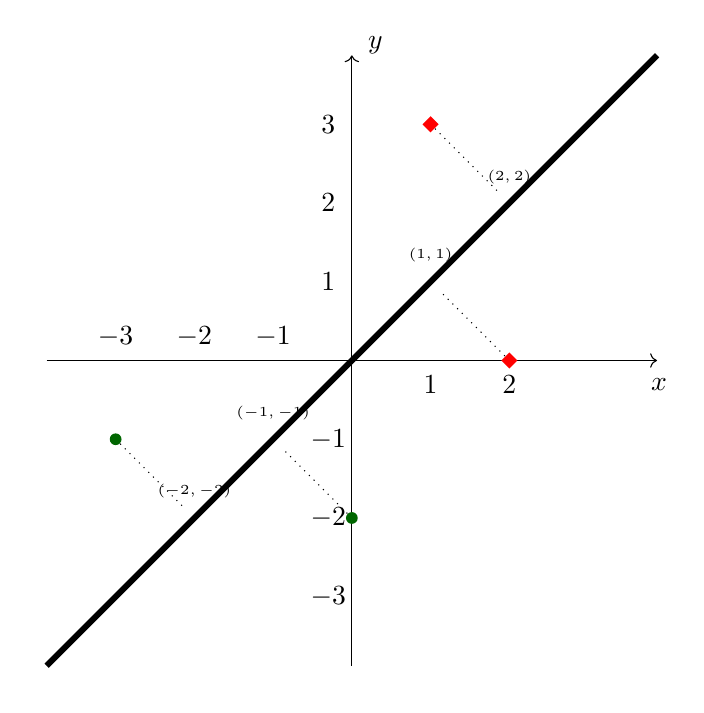
\begin{tikzpicture}
					\node (origin) at (0, 0) {};
					\node (top) at ($(origin) + (0, 4)$) {};
					\node (bottom) at ($(origin) + (0, -4)$) {};
					\node (left) at ($(origin) + (-4, 0)$) {};
					\node (right) at ($(origin) + (4, 0)$) {};
					\draw [->] (bottom) -- (top);
					\draw [->] (left) -- (right);
			
					\node at (-4, -4) (leftendpoint) {};
					\node at (4, 4) (rightendpoint) {};
					%\node at ($(origin) + (0.8, 1.3)$) {$y=\alpha x$};
					\node at ($(origin) + (3.9, -0.3)$) {$x$};
					\node at ($(origin) + (0.3, 4.0)$) {$y$};
			
					\draw[line width=0.75mm] (leftendpoint) -- (rightendpoint);
			
					\node[circle, fill=black!60!green, inner sep=1.5pt] at ($({-3/1.0}, {-1/1.0})$) (dp1) {};
					\node[circle, fill=black!60!green, inner sep=1.5pt] at ($({0/1.0}, {-2/1.0})$) (dp2) {};
					\node[diamond, fill=red, inner sep=1.5pt] at ($({2/1.0}, {0/1.0})$) (dp3) {};
					\node[diamond, fill=red, inner sep=1.5pt] at ($({1/1.0}, {3/1.0})$) (dp4) {};
					

					\node[label= {\tiny $\left( -2, -2\right)$}] at (-2, -2) (r1) {};
					\node[label= {\tiny $\left( -1, -1\right)$}] at (-1, -1) (r2) {};
					\node[label= {\tiny $\left( 1, 1\right)$}] at (1, 1) (r3) {};
					\node[label= {\tiny $\left( 2, 2\right)$}] at (2, 2) (r4) {};

					\draw[dotted] (dp1) -- (r1);
					\draw[dotted] (dp2) -- (r2);
					\draw[dotted] (dp3) -- (r3);
					\draw[dotted] (dp4) -- (r4);
			
					\node at ($({1/1.0}, 0.1)$) (dp1x) {};
					\node at ($(-0.1, {-2/1.0})$) (dp1y) {};
					\node at ($({1/1.0}, -0.3)$) {$1$};
					\node at ($(-0.3, {-2/1.0})$) {$-2$};
					%\draw[dotted] (dp1) -- (dp1x);
					%\draw[dotted] (dp1) -- (dp1y);
			
					\node at ($({2/1.0}, -0.1)$) (dp2x) {};
					\node at ($(-0.1, {3/1.0})$) (dp2y) {};
					\node at ($({2/1.0}, -0.3)$) {$2$};
					\node at ($(-0.3, {1/1.0})$) {$1$};
					\node at ($(-0.3, {2/1.0})$) {$2$};
					\node at ($(-0.3, {3/1.0})$) {$3$};
					%\draw[dotted] (dp2) -- (dp2x);
					%\draw[dotted] (dp2) -- (dp2y);
			
					\node at ($({-3/1.0}, 0.1)$) (dp3x) {};
					\node at ($(0.1, {-1/1.0})$) (dp3y) {};
					\node at ($({-3/1.0}, 0.3)$) {$-3$};
					\node at ($({-2/1.0}, 0.3)$) {$-2$};
					\node at ($({-1/1.0}, 0.3)$) {$-1$};
					\node at ($(-0.3, {-3/1.0} )$) {$-3$};
					\node at ($(-0.3, {-1/1.0} )$) {$-1$};
					%\draw[dotted] (dp3) -- (dp3x);
					%\draw[dotted] (dp3) -- (dp3y);
			
			
					\node[inner sep=0pt] at ($(leftendpoint)!(dp1)!(rightendpoint)$) (pdp1) {};
					\node[inner sep=0pt] at ($(leftendpoint)!(dp2)!(rightendpoint)$) (pdp2) {};
					\node[inner sep=0pt] at ($(leftendpoint)!(dp3)!(rightendpoint)$) (pdp3) {};
			
					%\draw[red] (dp1) -- (pdp1);
					%\draw[red] (dp2) -- (pdp2);
					%\draw[red] (dp3) -- (pdp3);
				\end{tikzpicture}
\end{Described}
				\caption{Plot of Transactions in 2-D}
			\end{figure}
		}


\end{enumerate}

  \newpage
  \qns{Diode System ID (Adapted from EECS 16B Fall 2023 Final)}

    \textbf{Note: This problem does not require knowledge of circuits or diodes.}
    
    Suppose that we want to characterize a diode $D_1$ with parasitic resistance $R_p$, represented by the following model:
    \begin{figure}[H]
        \begin{center}
            \begin{Described}{Voltage source V sub B drives from ground up to the top node, where diode D1 carries current I D to the right with voltage V D across it, in series with resistor R sub p returning to ground.}
\begin{circuitikz}
                \draw (0, 2) to [V, l_=$V_B$] (0, 0) node[ground]{}
                (0, 2) to [Do, l=$D_1$, i=$I_D$, v=$V_D$] (3, 2) to [R, l=$R_p$] (5, 2) node[ground]{}
                ;
            \end{circuitikz}
\end{Described}
        \end{center}
    \end{figure}
    The current through the diode (forward-biased) is modeled as
    \begin{equation}
        I_D = I_0\e^{\frac{V_D}{V_T}}
    \end{equation}
    where $V_D$ is the voltage across the diode (as shown in the diagram), $I_0$ is a parameter associated with the diode, and $V_T$ is the thermal voltage, a temperature dependent variable.
    
    With some analysis, the system equation can be simplified to:
    \begin{equation}
        I_D = I_0 \e^{\frac{V_B - I_D R_p}{V_T}}
    \end{equation}
    To collect data, we will vary the temperature to vary $V_T$ and measure the current $I_D$ through the diode.
    
        \begin{enumerate}

            \qitem    Use the provided system equation to show that
                \begin{equation}
                    I_D R_p - V_T \ln(I_0) = V_B - V_T \ln(I_D)
                \end{equation}
                    is a valid equation to represent the system.
                \begin{hint}
                    Use the logarithm identity $\ln(\frac{a}{b}) = \ln(a) - \ln(b)$.
                \end{hint}
            
    
            \ans{
                \begin{align}
                    I_D &= I_0 \e^{\frac{V_B - I_D R_p}{V_T}} \\
                    V_T\ln(\frac{I_D}{I_0}) &= V_B - I_D R_p \\
                    V_T\ln(I_D) - V_T\ln(I_0) &= V_B - I_D R_p \\
                    I_D R_p - V_T \ln(I_0) &= V_B - V_T \ln(I_D)
                \end{align}
            }
    
            % \begin{problempart}{4}{System ID}{0}{0}
            %     Suppose we use $V_B = 1 \mathrm{V}$ and collect the following data points:
            %     \begin{itemize}
            %         \item For $V_T = 0.025 \mathrm{V}$, $I_D = 0.0185 \mathrm{A}$.
            %         \item For $V_T = 0.05 \mathrm{V}$, $I_D = 0.0172 \mathrm{A}$.
            %         \item For $V_T = 0.0125 \mathrm{V}$, $I_D = 0.0193 \mathrm{A}$.
            %     \end{itemize}
            %     \textbf{Find the matrix $D$ and vector $\vec{s}$ to set up a least-squares problem $D\vec{p} \approx \vec{s}$ where $\vec{p} = \begin{bmatrix} \ln(I_0) \\ R_p \end{bmatrix}$.}
    
            %     You do not have to simplify the elements $D$ and $\vec{s}$, but the elements should be numerical values, not in terms of variables.
            % \end{problempart}
    
            % \begin{solution}{4in}
            %     Each data point can be used with the provided system equation from the first part to create a system of linear equations with the unknowns being $\ln(I_0)$ and $R_p$ (remember that the problem provides that $V_B = 1 \mathrm{V}$):
            %     \begin{itemize}
            %         \item $-0.025\ln(I_0) + 0.0185R_p = 1 - 0.025\ln(0.0185)$
            %         \item $-0.05\ln(I_0) + 0.0172R_p = 1 - 0.05\ln(0.0172)$
            %         \item $-0.0125\ln(I_0) + 0.0193R_p = 1 - 0.0125\ln(0.0193)$
            %     \end{itemize}
            %     The matrix form of this system is:
            %     \begin{equation}
            %         \begin{bmatrix} -0.025 & 0.0185 \\ -0.05 & 0.0172 \\ -0.0125 & 0.0193 \end{bmatrix} \begin{bmatrix} \ln(I_0) \\ R_p \end{bmatrix} = \begin{bmatrix} 1 - 0.025\ln(0.0185) \\ 1 - 0.05\ln(0.0172) \\ 1 - 0.0125\ln(0.0193) \end{bmatrix}
            %     \end{equation}
            %     Thus, for the least-squares problem, $D = \begin{bmatrix} -0.025 & 0.0185 \\ -0.05 & 0.0172 \\ -0.0125 & 0.0193 \end{bmatrix}$ and $\vec{s} = \begin{bmatrix} 1 - 0.025\ln(0.0185) \\ 1 - 0.05\ln(0.0172) \\ 1 - 0.0125\ln(0.0193) \end{bmatrix}$
            % \end{solution}
    
            \vspace{5cm}
            
            \qitem    Suppose we use $V_B = v_B$ and collect the following data points:
                \begin{itemize}
                    \item For $V_T = v_{T1}$, $I_D = i_{D1}$.
                    \item For $V_T = v_{T2}$, $I_D = i_{D2}$.
                    \item For $V_T = v_{T3}$, $I_D = i_{D3}$.
                \end{itemize}
                Find the matrix $\textbf{A}$ and vector $\vec{x}$ to set up a least-squares problem $\textbf{A} \vec{x} \approx \vec{b}$ where $\vec{x} = \begin{bmatrix} \ln(I_0) \\ R_p \end{bmatrix}$
    
            \ans{
                Each data point can be used with the provided system equation from the first part to create a system of linear equations with the unknowns being $\ln(I_0)$ and $R_p$ (remember that the problem provides that $V_B = v_B$):
                \begin{itemize}
                    \item $-v_{T1}\ln(I_0) + i_{D1}R_p = v_B - v_{T1}\ln(i_{D1})$
                    \item $-v_{T2}\ln(I_0) + i_{D2}R_p = v_B - v_{T2}\ln(i_{D2})$
                    \item $-v_{T3}\ln(I_0) + i_{D3}R_p = v_B - v_{T3}\ln(i_{D3})$
                \end{itemize}
                The matrix form of this system is:
                \begin{equation}
                    \begin{bmatrix} -v_{T1} & i_{D1} \\ -v_{T2} & i_{D2} \\ -v_{T3} & i_{D3} \end{bmatrix} \begin{bmatrix} \ln(I_0) \\ R_p \end{bmatrix} = \begin{bmatrix} v_B - v_{T1}\ln(i_{D1}) \\ v_B - v_{T2}\ln(i_{D2}) \\ v_B - v_{T3}\ln(i_{D3}) \end{bmatrix}
                \end{equation}
                Thus, for the least-squares problem, $\textbf{A} = \begin{bmatrix} -v_{T1} & i_{D1} \\ -v_{T2} & i_{D2} \\ -v_{T3} & i_{D3} \end{bmatrix}$ and $\vec{b} = \begin{bmatrix} v_B - v_{T1}\ln(i_{D1}) \\ v_B - v_{T2}\ln(i_{D2}) \\ v_B - v_{T3}\ln(i_{D3}) \end{bmatrix}$
            }
            
            \vspace{5cm}
            
            \qitem    Explain how you would use the least-squares system from the previous part to find model parameters $I_0$ and $R_p$. You do not need to use actual values for this part; you explanation can just use $\textbf{A}$ and $\vec{b}$ as known variables to show what calculations you would do to find $I_0$ and $R_p$.
            
    
            \ans{
                We would first find the optimal parameter $\hat{\vec{x}}$ with the least squares formula:
                \begin{equation}
                    \hat{\vec{x}} = (\textbf{A}^\top \textbf{A})^{-1} \textbf{A}^{\top} \vec{b}
                \end{equation}
                The elements of $\hat{\vec{x}}$ represent optimal values for $\ln(I_0)$ and $R_p$ so we set the elements of $\hat{\vec{x}}$ equal to those parameters for our model:
                \begin{align}
                    \hat{x}_{v_B} = \ln(I_0) &\rightarrow I_0 = \e^{\hat{x}_1} \\
                    \hat{x}_2 = R_p &\rightarrow R_p = \hat{x}_2
                \end{align}
                Thus, we have found parameter values for $I_0$ and $R_p$ from the least-squares system.
            }
    
        \end{enumerate}

\end{qunlist}

\end{document}
"
%   pdflatex "\PassOptionsToClass{prob}{latexally-assignment}% Demonstration built from REAL EECS 16A questionBank material, not from
% invented figures. Four question files were copied verbatim out of the corpus
% into corpus/ below, and `latexally apply` wrapped each figure in Described
% with a hand-written description. Nothing else in them was touched.
%
%   corpus/questionBank/sec/13/q_polynomial_fir_convolution.tex   1 figure
%   corpus/questionBank/sec/13/q_freq_resp_dag_diagram.tex        2 figures
%   corpus/sp26/dis/13A/questions/q_pca.tex                       4 figures
%   corpus/sp26/dis/13A/questions/q_diode_ls.tex                  1 figure
%
% Build both variants from this ONE source; build.sh supplies the class option:
%   pdflatex "\PassOptionsToClass{sol}{latexally-assignment}% Demonstration built from REAL EECS 16A questionBank material, not from
% invented figures. Four question files were copied verbatim out of the corpus
% into corpus/ below, and `latexally apply` wrapped each figure in Described
% with a hand-written description. Nothing else in them was touched.
%
%   corpus/questionBank/sec/13/q_polynomial_fir_convolution.tex   1 figure
%   corpus/questionBank/sec/13/q_freq_resp_dag_diagram.tex        2 figures
%   corpus/sp26/dis/13A/questions/q_pca.tex                       4 figures
%   corpus/sp26/dis/13A/questions/q_diode_ls.tex                  1 figure
%
% Build both variants from this ONE source; build.sh supplies the class option:
%   pdflatex "\PassOptionsToClass{sol}{latexally-assignment}\input{demo-questionbank}"
%   pdflatex "\PassOptionsToClass{prob}{latexally-assignment}\input{demo-questionbank}"

\DocumentMetadata{
  lang       = en-US,
  pdfversion = 2.0,
  testphase  = {phase-III,math,table,graphic,firstaid},
}
\documentclass{latexally-assignment}

\usepackage{amsmath,amssymb}
\usepackage{float}
\usepackage{tikz}
\usetikzlibrary{calc,shapes.geometric,positioning}
\usepackage[american]{circuitikz}

% The corpus macros these four files use, reproduced from questionBank/ee16.sty
% and questionBank/sp26/sp26.sty so the demo does not need the whole course
% preamble chain. Same meanings, nothing more.
\providecommand{\bmqty}[1]{\begin{bmatrix}#1\end{bmatrix}}
\providecommand{\e}{\mathop{\mathrm{e}}\nolimits}
\providecommand{\wt}[1]{\widetilde{#1}}
\NewDocumentEnvironment{hint}{+b}{\itshape (HINT: #1)}{}

\setcoursenumber{EECS 16A}
\setcoursename{Designing Information Devices and Systems I}
\setsemester{Spring 2026}

\begin{document}

\def\title{Described figures from the question bank}
\maketitle

\vspace{0.5em}
Every figure below carries a description in the PDF structure tree. A screen
reader announces "graphic" and then that description; it never reaches the
drawing underneath. Hovering shows nothing --- \texttt{/Alt} is not a tooltip.

\begin{qunlist}

  \input{corpus/questionBank/sec/13/q_polynomial_fir_convolution.tex}
  \newpage
  \input{corpus/questionBank/sec/13/q_freq_resp_dag_diagram.tex}
  \newpage
  \input{corpus/sp26/dis/13A/questions/q_pca.tex}
  \newpage
  \input{corpus/sp26/dis/13A/questions/q_diode_ls.tex}

\end{qunlist}

\end{document}
"
%   pdflatex "\PassOptionsToClass{prob}{latexally-assignment}% Demonstration built from REAL EECS 16A questionBank material, not from
% invented figures. Four question files were copied verbatim out of the corpus
% into corpus/ below, and `latexally apply` wrapped each figure in Described
% with a hand-written description. Nothing else in them was touched.
%
%   corpus/questionBank/sec/13/q_polynomial_fir_convolution.tex   1 figure
%   corpus/questionBank/sec/13/q_freq_resp_dag_diagram.tex        2 figures
%   corpus/sp26/dis/13A/questions/q_pca.tex                       4 figures
%   corpus/sp26/dis/13A/questions/q_diode_ls.tex                  1 figure
%
% Build both variants from this ONE source; build.sh supplies the class option:
%   pdflatex "\PassOptionsToClass{sol}{latexally-assignment}\input{demo-questionbank}"
%   pdflatex "\PassOptionsToClass{prob}{latexally-assignment}\input{demo-questionbank}"

\DocumentMetadata{
  lang       = en-US,
  pdfversion = 2.0,
  testphase  = {phase-III,math,table,graphic,firstaid},
}
\documentclass{latexally-assignment}

\usepackage{amsmath,amssymb}
\usepackage{float}
\usepackage{tikz}
\usetikzlibrary{calc,shapes.geometric,positioning}
\usepackage[american]{circuitikz}

% The corpus macros these four files use, reproduced from questionBank/ee16.sty
% and questionBank/sp26/sp26.sty so the demo does not need the whole course
% preamble chain. Same meanings, nothing more.
\providecommand{\bmqty}[1]{\begin{bmatrix}#1\end{bmatrix}}
\providecommand{\e}{\mathop{\mathrm{e}}\nolimits}
\providecommand{\wt}[1]{\widetilde{#1}}
\NewDocumentEnvironment{hint}{+b}{\itshape (HINT: #1)}{}

\setcoursenumber{EECS 16A}
\setcoursename{Designing Information Devices and Systems I}
\setsemester{Spring 2026}

\begin{document}

\def\title{Described figures from the question bank}
\maketitle

\vspace{0.5em}
Every figure below carries a description in the PDF structure tree. A screen
reader announces "graphic" and then that description; it never reaches the
drawing underneath. Hovering shows nothing --- \texttt{/Alt} is not a tooltip.

\begin{qunlist}

  \input{corpus/questionBank/sec/13/q_polynomial_fir_convolution.tex}
  \newpage
  \input{corpus/questionBank/sec/13/q_freq_resp_dag_diagram.tex}
  \newpage
  \input{corpus/sp26/dis/13A/questions/q_pca.tex}
  \newpage
  \input{corpus/sp26/dis/13A/questions/q_diode_ls.tex}

\end{qunlist}

\end{document}
"

\DocumentMetadata{
  lang       = en-US,
  pdfversion = 2.0,
  testphase  = {phase-III,math,table,graphic,firstaid},
}
\documentclass{latexally-assignment}

\usepackage{amsmath,amssymb}
\usepackage{float}
\usepackage{tikz}
\usetikzlibrary{calc,shapes.geometric,positioning}
\usepackage[american]{circuitikz}

% The corpus macros these four files use, reproduced from questionBank/ee16.sty
% and questionBank/sp26/sp26.sty so the demo does not need the whole course
% preamble chain. Same meanings, nothing more.
\providecommand{\bmqty}[1]{\begin{bmatrix}#1\end{bmatrix}}
\providecommand{\e}{\mathop{\mathrm{e}}\nolimits}
\providecommand{\wt}[1]{\widetilde{#1}}
\NewDocumentEnvironment{hint}{+b}{\itshape (HINT: #1)}{}

\setcoursenumber{EECS 16A}
\setcoursename{Designing Information Devices and Systems I}
\setsemester{Spring 2026}

\begin{document}

\def\title{Described figures from the question bank}
\maketitle

\vspace{0.5em}
Every figure below carries a description in the PDF structure tree. A screen
reader announces "graphic" and then that description; it never reaches the
drawing underneath. Hovering shows nothing --- \texttt{/Alt} is not a tooltip.

\begin{qunlist}

  \qns{Polynomial Multiplication and Discrete-Time Convolution [Adapted from EE 120]}
% Adapted and extended by Ken Zheng for EECS 16A Fall 2025 Discussion

The impulse response of a real, discrete-time FIR filter $\mathsf{A}$ is described by  
$$a[n]=a_0 \delta[n]+a_1 \delta[n-1]+\cdots + a_N \delta[n-N], \quad \text{where } N\in \{1,2,3,\ldots\}.$$

\begin{enumerate}[(a)]
\item Show that the frequency response $A(\omega)$ of the filter is a polynomial, in terms of $e^{-i\omega}$, whose coefficients have a simple relationship with the impulse response values $a_0,\ldots,a_N$.

\ans{

    Substituting \(a[n]\) into the frequency response formula we see that:
    \begin{equation*}
        A(w) = \sum_{n=-\infty}^{\infty} a[n]e^{-iwn}
    \end{equation*}
    As $a[n] = 0$ outside the range of $n = 0$ to $n = N$ ,
    \begin{equation*}
        A(w) = a_0 e^{-iw\cdot 0} + a_1 e^{-iw\cdot 1} + \ldots + a_N e^{-iw\cdot N}
    \end{equation*}
    \begin{equation*}
        = a_0 + a_1 e^{-iw} + \ldots + a_N e^{-iwN}
    \end{equation*}
}
\item Suppose the filter $\mathsf{A}$ is placed in a cascade (series) interconnection with another discrete-time FIR filter $\mathsf{B}$ whose impulse response is described by  
$$b[n]=b_0 \delta[n]+b_1 \delta[n-1]+\cdots + b_M \delta[n-M],\quad \text{where } M\in \{1,2,3,\ldots\}.$$

The cascade structure, which we call $\mathsf{C}$, is shown in the figure below.
\vspace{4pt}

\centerline{
    \begin{Described}{Block diagram: input x enters block A, whose output feeds block B, and block B's output is y. An outer box enclosing both blocks is labelled C.}
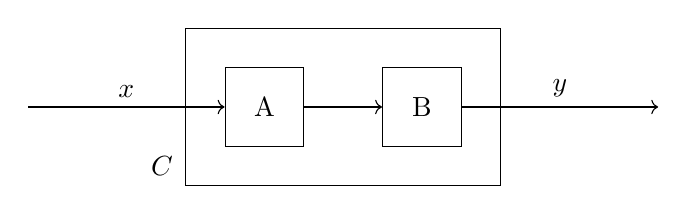
\begin{tikzpicture}
        % Define nodes for blocks A and B
        \node[draw, rectangle, minimum width=1cm, minimum height=1cm] (A) at (0,0) {A};
        \node[draw, rectangle, minimum width=1cm, minimum height=1cm] (B) at (2,0) {B};
        
        % Draw the outer rectangle
        \draw (-1, 1) rectangle (3, -1);
        
        % Draw arrows and labels
        \draw[->] (-3, 0) -- (A.west) node[midway,above] {$x$};
        \draw[->] (A.east) -- (B.west);
        \draw[->] (B.east) -- (5, 0) node[midway,above] {$y$};
        
        % Label C 
        \node at (-1.3, -0.5) [below] {$C$};
    \end{tikzpicture}
\end{Described}
}
Let $c$ denote the impulse response of the cascade interconnection.

\begin{enumerate}[(i)]
\item Express $c$ in terms of $a$ and $b$.
    
\ans{

        The impulse response \(c\) of the cascade interconnection is given by 
        \begin{equation*}
            c[n] = (a * b)[n] = \sum_{k=-\infty}^{\infty} a[k]\,b[n-k]
        \end{equation*}
         Substituting \(n = 0\):
        \begin{equation*}
            c_0 = a_0 b_0
        \end{equation*}
        \(n = 1\):
        \begin{equation*}
            c_1 = a_0 b_1 + a_1 b_0 
        \end{equation*}
        \(n = 2\):
        \begin{equation*}
            c_2 = a_0 b_2 + a_1 b_1 + a_2 b_0
        \end{equation*}
        And so on...
    
        Thus, we can write:
        \begin{equation*}
            c_n = \sum_{k=\max(0,n-M)}^{\min(n, N)} a_k b_{n-k}
        \end{equation*}
        \null\hfill for \(n = 0, 1, \ldots, N + M\)
        
        where we found the bounds of summation from the two conditions that ensure we are indexing \(a[n]\) and \(b[n]\) without exceeding the bounds of their signal.
        $$ 0 \leq k \leq N \Longrightarrow k \leq N \quad \text{and} \quad k \geq 0 $$
        $$ 0 \leq n - k \leq M \Longrightarrow k \leq n \quad \text{and} \quad k \geq n - M $$
        and so
        $$ k \leq \min(n, N) \quad \text{and} \quad k \geq \max(0, n-M) $$

        Lastly, 
         \begin{equation*}
            c[n] = c_0\delta[n] + c_1 \delta[n - 1] + ... + c_{N + M} \delta[n - ( N + M)]
        \end{equation*}
        
    }

\item Consider two polynomials $A(z)$ and $B(z)$ described as follows:
    $$
    A(z) = a_0 +a_1 z + \cdots + a_N z^N \quad \quad \quad B(z) = b_0 +b_1 z + \cdots + b_M z^M \, ,
    $$
    where $M$ and $N$ and positive integers.
    Let $C(z)=A(z)\, B(z)$, where $$ C(z) = c_0 +c_1 z + \cdots + c_{N+M} z^{N+M}.$$  Show that multiplying polynomials is tantamount to convolving their coefficients; in particular, explain how $c_n=(a*b)_n=\displaystyle\sum_m a_m b_{n-m}$, where $n={0,1,\ldots, N+M}$.
    
    \ans{
    \begin{equation*}
        C(z) = (a_0 +a_1 z + \cdots + a_N z^N) (b_0 +b_1 z + \cdots + b_M z^M)
    \end{equation*}
    \begin{equation*}
        C(z) = a_0 b_0 + (a_0 b_1 + a_1 b_0) z + (a_0 b_2 + a_1 b_1 + a_2 b_0) z^2 + ...
    \end{equation*}
    As you can see, each coefficient of \(z^n\) is the sum of all products of \(a_i\) and \(b_j\) where \(i + j = n\):
    \begin{equation*}
        c_n =  \sum_{m=\max(0,n-M)}^{\min(n, N)} a_m b_{n-m}
    \end{equation*}
    \null\hfill for \(n = 0, 1, 2, ..., N + M\)

    Just like the definition of convolution!
    }

\end{enumerate}
\end{enumerate}
  \newpage
  \qns{Frequency Response from a DAG Block Diagram [Adapted from EE 120]}
% Adapted by Ken Zheng for EECS 16A Fall 2025 Discussion

    Consider a DT LTI system with input $x[n]$ and output $y[n]$ that is implemented by the following block diagram:
    \begin{figure}[h!]
      \centering
      \begin{Described}{Block diagram: input x of n enters a summing junction whose output is y of n. That output is tapped, passed through a delay block D and then a gain of minus 0.5, and fed back into the summing junction.}
\begin{circuitikz}
          \node (x) at (0, 0) {$x[n]$};
          \node[circle, draw] (sum) at (2, 0) {$+$};
          % FIXME: find a better way to draw the triangle
          % \node[triangleblock, shape border rotate=90, inner sep=-1mm] (gain) at (3, -1.5) {$-0.5$};
          % \node at (3, -1.5) {$-0.5$};
          \node[draw, inner sep=5pt] (delay) at (6, -1.5) {$D$};
          \node (y) at (9, 0) {$y[n]$};
          \draw[->] (x.east) -- (sum.west);
          \draw[->] (sum.east) -- (y.west);
          \draw[->] (7.5, 0) -- (7.5, -1.5) -- (delay.east);
          % \draw[-, thick] (delay.west) -- (gain.east);
          % \draw[->, thick] (gain.west) -- (2, -1.5) -- (sum.south);
          \draw[->] (delay.west) to [amp, t=$-0.5$, blocks/scale=1.5] (2, -1.5) to (sum.south);
      \end{circuitikz}
\end{Described}
  \end{figure}
\begin{enumerate}
        \item Find the LCCDE that describes this system. 
        
        \ans{
            The difference equation describing this system is
              \begin{equation*}
                y[n] = x[n] - 0.5y[n-1]
              \end{equation*}
        }

        \item Find the frequency response $H(\omega)$ of this system. 
            
        \ans{
            Using the eigenfunction property by setting $x[n] = e^{i\omega n}$ and $y[n] = H(\omega) e^{i\omega n}$,
            \begin{align*}
            H(\omega) e^{i\omega n} &= e^{i\omega n} - 0.5 H(\omega) e^{i\omega (n-1)} \\
            &= e^{i\omega n} - 0.5 H(\omega) e^{-i\omega}e^{i\omega n} \\
            \left(1 + 0.5 e^{-i\omega}\right) e^{i\omega n} H(\omega) &= e^{i\omega n} \\
            H(\omega) &= \frac{e^{i\omega n}}{\left(1 + 0.5 e^{-i\omega}\right)e^{i\omega n}} \\
                &= \frac{1}{1 + 0.5 e^{-i\omega}}
            \end{align*} 
        } 

        \vspace{4cm}

        \item Is this a high pass or low pass filter?
        
        \ans{
            We can think about this in two ways:
            
            \textbf{1. Geometric Approach:}

            Recall from part (b) that the frequency response can be written as:
            \[
            H(\omega) = \frac{1}{1 + 0.5 e^{-i\omega}} = \frac{e^{i\omega}}{e^{i\omega} - (-0.5)}
            \]
            The magnitude is therefore:
            \[
            |H(\omega)| = \frac{1}{|e^{i\omega} - (-0.5)|}
            \]
            This represents the reciprocal of the distance from the point $e^{i\omega}$ on the unit circle to the point located at $-0.5$ on the real axis:

            \begin{center}
            \begin{Described}{Complex plane with real and imaginary axes and the unit circle centred at the origin. A point is marked at minus 0.5 on the real axis, with an arrow from it to the point e to the i omega on the circle.}
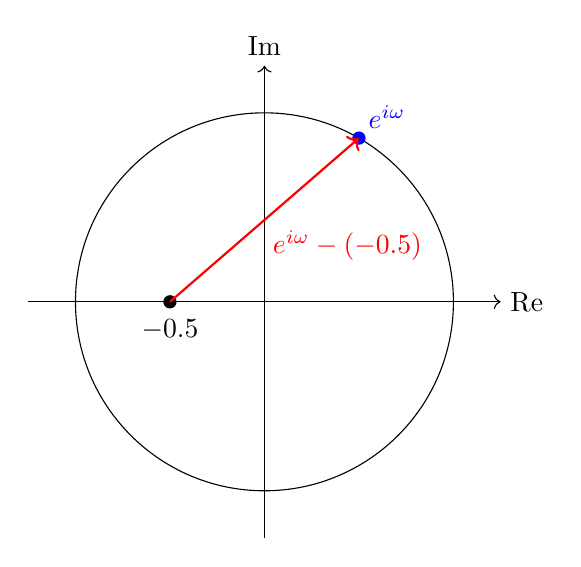
\begin{tikzpicture}[scale=1.2]
                % Axes
                \draw[->] (-2.5,0) -- (2.5,0) node[right] {$\operatorname{Re}$};
                \draw[->] (0,-2.5) -- (0,2.5) node[above] {$\operatorname{Im}$};

                % Unit circle
                \draw (0,0) circle (2);

                % Pole at -0.5
                \fill[black] (-1,0) circle (2pt) node[below left] {};
                \node[black] at (-1,-0.3) {$-0.5$};

                % Point on unit circle at angle ω
                \coordinate (P) at (60:2);
                \fill[blue] (P) circle (2pt) node[above right] {$e^{i\omega}$};

                % Vector from pole to point on circle
                % \draw[->, thick, red] (-1,0) -- (P);
                \draw[->, thick, red] (-1,0) -- (P) node[midway, below] {$\qquad\qquad\qquad e^{i \omega} - (-0.5)$};  % Label added here


                % Labels
                \node at (1.8,1.8) {};
            \end{tikzpicture}
\end{Described}
            \end{center}

            Key observations:
            \begin{itemize}
                \item When $\omega = 0$, $e^{i\omega} = 1$. The distance from $1$ to $-0.5$ is $1.5$, so $|H(0)| = 1/1.5 \approx 0.667$.
                \item When $\omega = \pi$, $e^{i\omega} = -1$. The distance from $-1$ to $-0.5$ is $0.5$, so $|H(\pi)| = 1/0.5 = 2$.
                \item As $\omega$ moves from $0$ to $\pi$, the point $e^{i\omega}$ travels along the upper half of the unit circle from $(1,0)$ to $(-1,0)$. 
                The distance to the point at $-0.5$ decreases monotonically, so $|H(\omega)|$ increases. Thus, we have a high-pass filter!\\
            \end{itemize}

            
            \textbf{2. Algebraic Approach:}
            
            To determine the filter type, we simplify the magnitude of the frequency response first:

            \[
            |H(\omega)| = \frac{1}{\sqrt{(1 + 0.5\cos\omega)^2 + (0.5\sin\omega)^2}}
            \]


            Expanding \( (1 + 0.5\cos\omega)^2 \) and \( (0.5\sin\omega)^2 \):
            \[
            (1 + 0.5\cos\omega)^2 = 1^2 + 2(1)(0.5\cos\omega) + (0.5\cos\omega)^2 = 1 + \cos\omega + 0.25\cos^2\omega
            \]
            \[
            (0.5\sin\omega)^2 = 0.25\sin^2\omega
            \]


            Add the two results in the square root:
            \[
            (1 + 0.5\cos\omega)^2 + (0.5\sin\omega)^2 = \left[1 + \cos\omega + 0.25\cos^2\omega\right] + \left[0.25\sin^2\omega\right]
            \]
            \[
            = 1 + \cos\omega + 0.25\left(\cos^2\omega + \sin^2\omega\right)
            \]
            \[
            = 1 + \cos\omega + 0.25(1) = 1 + \cos\omega + 0.25 = 1.25 + \cos\omega
            \]


            Substitute back into \( |H(\omega)| \):
            \[
            |H(\omega)| = \frac{1}{\sqrt{1.25 + \cos\omega}}
            \]
                        
            Now we analyze the magnitude at key frequencies:
            
            Low frequency (\( \omega = 0 \)): 
                \[
                |H(0)| =  \frac{1}{\sqrt{1.25 + \cos0}} = \frac{1}{1.5} \approx 0.667 \quad (\text{attenuated})
                \]
            High frequency (\( \omega = \pi \)): 
                \[
                |H(\pi)| =  \frac{1}{\sqrt{1.25 + \cos\pi}} = 2 \quad (\text{passed})
                \]

            We can see that, again, the filter attenuates low frequencies and passes high frequencies, so it is a high-pass filter!\\

            Both geometrically and algebraically, we conclude this is a \textbf{high-pass filter}. Nice!
        }
\end{enumerate}

  \newpage
  \qns{Using PCA to Detect Fraudulent Transactions (Adapted from EECS 16B Spring 2023 Final)}\\
	PCA has many different uses when applied to real-world data. One potential application is making classification of data much easier.
	
	Suppose we are given some data, where each datapoint represents a transaction. Each one is labeled either normal or fraudulent. We will utilize PCA to develop a useful classifier.

	We plot the data in two dimensions, where each dimension is some unspecified feature that will aid us in classifying the points:

	\begin{figure}[H]
        \centering
        \begin{Described}{Scatter plot on x and y axes running about minus 4 to 4, with four transactions marked: circles at (-3, -1) and (0, -2), and diamonds at (2, 0) and (1, 3).}
\begin{tikzpicture}
            \node (origin) at (0, 0) {};
            \node (top) at ($(origin) + (0, 4)$) {};
            \node (bottom) at ($(origin) + (0, -4)$) {};
            \node (left) at ($(origin) + (-4, 0)$) {};
            \node (right) at ($(origin) + (4, 0)$) {};
            \draw [->] (bottom) -- (top);
            \draw [->] (left) -- (right);
    
            \node at (-3, -2.2) (leftendpoint) {};
            \node at (3, 2.2) (rightendpoint) {};
            %\node at ($(origin) + (0.8, 1.3)$) {$y=\alpha x$};
            \node at ($(origin) + (3.9, -0.3)$) {$x$};
            \node at ($(origin) + (0.3, 4.0)$) {$y$};
    
            %\draw[line width=0.75mm] (leftendpoint) -- (rightendpoint);
    
            \node[circle, fill=black!60!green, inner sep=1.5pt] at ($({-3/1.0}, {-1/1.0})$) (dp1) {};
            \node[circle, fill=black!60!green, inner sep=1.5pt] at ($({0/1.0}, {-2/1.0})$) (dp2) {};
            \node[diamond, fill=red, inner sep=1.5pt] at ($({1/1.0}, {3/1.0})$) (dp3) {};
			\node[diamond, fill=red, inner sep=1.5pt] at ($({2/1.0}, {0/1.0})$) (dp4) {};
    
            \node at ($({1/1.0}, 0.1)$) (dp1x) {};
            \node at ($(-0.1, {-2/1.0})$) (dp1y) {};
            \node at ($({1/1.0}, 0.3)$) {$1$};
            \node at ($(-0.3, {-2/1.0})$) {$-2$};
            %\draw[dotted] (dp1) -- (dp1x);
            %\draw[dotted] (dp1) -- (dp1y);
    
            \node at ($({2/1.0}, -0.1)$) (dp2x) {};
            \node at ($(-0.1, {3/1.0})$) (dp2y) {};
            \node at ($({2/1.0}, -0.3)$) {$2$};
            \node at ($(-0.3, {3/1.0})$) {$3$};
            %\draw[dotted] (dp2) -- (dp2x);
            %\draw[dotted] (dp2) -- (dp2y);
    
            \node at ($({-3/1.0}, 0.1)$) (dp3x) {};
            \node at ($(0.1, {-1/1.0})$) (dp3y) {};
            \node at ($({-3/1.0}, 0.3)$) {$-3$};
            \node at ($(-0.3, {-1/1.0 -0.3} )$) {$-1$};
            %\draw[dotted] (dp3) -- (dp3x);
            %\draw[dotted] (dp3) -- (dp3y);
    
    
            \node[inner sep=0pt] at ($(leftendpoint)!(dp1)!(rightendpoint)$) (pdp1) {};
            \node[inner sep=0pt] at ($(leftendpoint)!(dp2)!(rightendpoint)$) (pdp2) {};
            \node[inner sep=0pt] at ($(leftendpoint)!(dp3)!(rightendpoint)$) (pdp3) {};
    
            %\draw[red] (dp1) -- (pdp1);
            %\draw[red] (dp2) -- (pdp2);
            %\draw[red] (dp3) -- (pdp3);
        \end{tikzpicture}
\end{Described}
        \caption{Plot of Transactions in 2-D}
	\end{figure}

	Thus, we have a total of 4 transactions, $\bmqty{-3 \\ -1}$ and $\bmqty{0 \\ -2}$ are normal, while $\bmqty{2 \\ 0}$ and $\bmqty{1 \\ 3}$ are fraudulent.
	\begin{enumerate}
		%Part A:
		
		\qitem Suppose we now construct a data matrix, where the \textit{data points are columns}. 

			\begin{equation}
				X = \bmqty{-3 & 0 & 2 & 1 \\ -1 & -2 & 0 & 3}
			\end{equation}

			Using this data matrix, \textbf{calculate its first principal component $\vec{u}_1$}.

			\begin{hint}
			\begin{enumerate}

				\item You may also make use of the fact that $XX^T$ is given by:
				\begin{align}
					XX^{\top} &= \bmqty{-3 & 0 & 2 & 1 \\ -1 & -2 & 0 & 3}\bmqty{-3 & 0 & 2 & 1 \\ -1 & -2 & 0 & 3}^{\top} \\
						&= \bmqty{14 & 6 \\ 6 & 14}
				\end{align}
				\item You may also make use of the characteristic polynomial of $XX^T$:
				\begin{equation}
					\lambda^2 - 28\lambda + 160 = (\lambda - 20)(\lambda - 8) = 0
				\end{equation}
			\end{enumerate}
			\end{hint}
			
			\begin{hint} Remember that your principal component should be of unit norm. \end{hint}

		\ans{
			% From PCA, we know that our first principal component of a matrix with column data is the first column vector of $U$ in the SVD of $X$. Thus, we use the SVD method of calculation (find the eigenvector corresponding to the largest eigenvalue of $XX^{\top}$ and normalize to yield $\vec{u}_1$).

			% \begin{align}
			% 	XX^{\top} &= \bmqty{-3 & 0 & 2 & 1 \\ -1 & -2 & 0 & 3}\bmqty{-3 & 0 & 2 & 1 \\ -1 & -2 & 0 & 3}^{\top} \\
			% 		 &= \bmqty{14 & 6 \\ 6 & 14}
			% \end{align}

			% From setting $\mathrm{det}(XX^{\top} - \lambda I) = 0$, we should find our characteristic polynomial to be 
			
			% \begin{equation}
			% 	\lambda^2 - 28\lambda + 160 = 0
			% \end{equation}

			Our eigenvalues are $\lambda_1 = 20$ and $\lambda_2 = 8$. Thus, the eigenvector corresponding to our largest eigenvalue $\lambda_1 = 20$ is $\vec{v}_1 = \bmqty{1 \\ 1}$ from inspection.
			
			Thus, our principal component vector is given as the normalized eigenvector: i.e. $\vec{u}_1 = \bmqty{\frac{1}{\sqrt{2}} \\ \frac{1}{\sqrt{2}}}$.
        }

		%Part B:
		
		\qitem	It's difficult to come up with a useful classifier in two dimensions. Let's use PCA dimensionality reduction to help.
			
			Using your answer in part (a), \textbf{project your two-dimensional data points onto one dimension. Express your answer as the vector $\vec{z} \in \mathbb{R}^{1 \times 4}$.}

		\ans{
			To project our 2-d data into 1-d, we project our data matrix onto the first principal component as follows:
			
			\begin{equation}
				\vec{z} = \vec{u}_1^{\top}X = \bmqty{\frac{1}{\sqrt{2}} \\ \frac{1}{\sqrt{2}}} \bmqty{-3 & 0 & 2 & 1 \\ -1 & -2 & 0 & 3} = \bmqty{-\frac{4}{\sqrt{2}} & -\frac{2}{\sqrt{2}} & \frac{2}{\sqrt{2}} & \frac{4}{\sqrt{2}}}
			\end{equation}
		}
		
		%Part C:
		
		\qitem	Now, plot each of these points, on the line below. Indicate the value and label (normal as circle and fraudulent as diamond) for each point.
			
			\textit{Note: your plot doesn't have to be to scale.}

			\begin{figure}[H]
				\centering
				\begin{Described}{Blank horizontal number line labelled z, with only the origin marked 0 and no points plotted.}
\begin{tikzpicture}
					\node (origin) at (0, 0) {|};
            		%\node (top) at ($(origin) + (0, 4)$) {};
            		%\node (bottom) at ($(origin) + (0, -4)$) {};
            		\node (left) at ($(origin) + (-4, 0)$) {};
            		\node (right) at ($(origin) + (4, 0)$) {};
					\node at ($(origin) + (3.9, -0.3)$) {$z$};
					\node at ($(origin) + (0, -0.3)$) {0};
            		%\draw [->] (bottom) -- (top);
            		\draw [<->] (left) -- (right);

				\end{tikzpicture}
\end{Described}
				\caption{Plot of Transactions in 1-D}
			\end{figure}

		\ans{
			\begin{figure}[H]
				\centering
				\begin{Described}{Number line labelled z with the origin marked 0 and four points: circles at minus four over root two and minus two over root two, diamonds at two over root two and four over root two.}
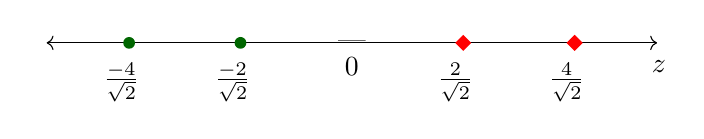
\begin{tikzpicture}
					\node (origin) at (0, 0) {|};
            		%\node (top) at ($(origin) + (0, 4)$) {};
            		%\node (bottom) at ($(origin) + (0, -4)$) {};
            		\node (left) at ($(origin) + (-4, 0)$) {};
            		\node (right) at ($(origin) + (4, 0)$) {};
					\node at ($(origin) + (3.9, -0.3)$) {$z$};
					\node at ($(origin) + (0, -0.3)$) {0};
            		%\draw [->] (bottom) -- (top);
            		\draw [<->] (left) -- (right);

					\node[circle, fill=black!60!green, inner sep=1.5pt] at ($(origin) + (-4/1.414, 0)$) (dp1) {};
					\node at ($(origin) + (-4/1.414 -0.1, -0.5)$) {$\frac{-4}{\sqrt{2}}$};
					\node[circle, fill=black!60!green, inner sep=1.5pt] at ($(origin) + (-2/1.414, 0)$) (dp1) {};
					\node at ($(origin) + (-2/1.414 -0.1, -0.5)$) {$\frac{-2}{\sqrt{2}}$};
					\node[diamond, fill=red, inner sep=1.5pt] at ($(origin) + (2/1.414, 0)$) (dp1) {};
					\node at ($(origin) + (2/1.414 -0.1, -0.5)$) {$\frac{2}{\sqrt{2}}$};
					\node[diamond, fill=red, inner sep=1.5pt] at ($(origin) + (4/1.414, 0)$) (dp1) {};
					\node at ($(origin) + (4/1.414 -0.1, -0.5)$) {$\frac{4}{\sqrt{2}}$};
				\end{tikzpicture}
\end{Described}
				\caption{Plot of Transactions in 1-D}
			\end{figure}
		}

		%Part D:
		
		\qitem	Suppose you are given some transaction datapoint, $\vec{x}_i$ and you project it to be one-dimensional, i.e. $z_i$. \textbf{Based on your plot from part (c), come up with an inequality in terms of $z_i$ to identify if that transaction is fraudulent.}
			
			\textit{Note: There can be more than one answer, but please only give one.}

		\ans{
			$\vec{z}_i > 0$ is a possible answer. In fact any answer in between $\vec{z}_i \geq -\frac{2}{\sqrt{2}}$ and $\vec{z}_i \geq \frac{2}{\sqrt{2}}$ is valid.
		}

		%Part E:
		
		\qitem	It can often be informative to compare our original data with its PCA reconstructions. \textbf{Using PCA, reconstruct $\vec{z}$ back into 2-D as the matrix $\wt{X} \in \mathbb{R}^{2 \times 4}$.}

		\ans{
			Using the reconstruction principle of PCA, we lift the 1D data back into 2 dimensions by doing the following:
			\begin{equation}
				\wt{X} = \vec{u}_1\vec{u}_1^{\top}X = \bmqty{-2 & -1 & 1 & 2 \\ -2 & -1 & 1 & 2}
			\end{equation}
		}

		%Part F:
		
		\qitem	Finally, we visualize our PCA reconstruction. \textbf{On the graph below, draw your first principal component direction (extend it as a solid line in both directions). Draw your reconstructioned points from $\wt{X}$, with dotted lines connecting them with the corresponding point in $X$. } You may draw on the plot on the next page.

			\begin{figure}[H]
				\centering
				\begin{Described}{Scatter plot on x and y axes running about minus 4 to 4, with four transactions marked: circles at (-3, -1) and (0, -2), and diamonds at (2, 0) and (1, 3).}
\begin{tikzpicture}
					\node (origin) at (0, 0) {};
					\node (top) at ($(origin) + (0, 4)$) {};
					\node (bottom) at ($(origin) + (0, -4)$) {};
					\node (left) at ($(origin) + (-4, 0)$) {};
					\node (right) at ($(origin) + (4, 0)$) {};
					\draw [->] (bottom) -- (top);
					\draw [->] (left) -- (right);
			
					\node at (-3, -2.2) (leftendpoint) {};
					\node at (3, 2.2) (rightendpoint) {};
					%\node at ($(origin) + (0.8, 1.3)$) {$y=\alpha x$};
					\node at ($(origin) + (3.9, -0.3)$) {$x$};
					\node at ($(origin) + (0.3, 4.0)$) {$y$};
			
					%\draw[line width=0.75mm] (leftendpoint) -- (rightendpoint);
			
					\node[circle, fill=black!60!green, inner sep=1.5pt] at ($({-3/1.0}, {-1/1.0})$) (dp1) {};
					\node[circle, fill=black!60!green, inner sep=1.5pt] at ($({0/1.0}, {-2/1.0})$) (dp2) {};
					\node[diamond, fill=red, inner sep=1.5pt] at ($({1/1.0}, {3/1.0})$) (dp3) {};
					\node[diamond, fill=red, inner sep=1.5pt] at ($({2/1.0}, {0/1.0})$) (dp4) {};
			
					\node at ($({1/1.0}, 0.1)$) (dp1x) {};
					\node at ($(-0.1, {-2/1.0})$) (dp1y) {};
					\node at ($({1/1.0}, 0.3)$) {$1$};
					\node at ($(-0.3, {-2/1.0})$) {$-2$};
					%\draw[dotted] (dp1) -- (dp1x);
					%\draw[dotted] (dp1) -- (dp1y);
			
					\node at ($({2/1.0}, -0.1)$) (dp2x) {};
					\node at ($(-0.1, {3/1.0})$) (dp2y) {};
					\node at ($({2/1.0}, -0.3)$) {$2$};
					\node at ($(-0.3, {3/1.0})$) {$3$};
					%\draw[dotted] (dp2) -- (dp2x);
					%\draw[dotted] (dp2) -- (dp2y);
			
					\node at ($({-3/1.0}, 0.1)$) (dp3x) {};
					\node at ($(0.1, {-1/1.0})$) (dp3y) {};
					\node at ($({-3/1.0}, 0.3)$) {$-3$};
					\node at ($(-0.3, {-1/1.0 -0.3} )$) {$-1$};
					%\draw[dotted] (dp3) -- (dp3x);
					%\draw[dotted] (dp3) -- (dp3y);
			
			
					\node[inner sep=0pt] at ($(leftendpoint)!(dp1)!(rightendpoint)$) (pdp1) {};
					\node[inner sep=0pt] at ($(leftendpoint)!(dp2)!(rightendpoint)$) (pdp2) {};
					\node[inner sep=0pt] at ($(leftendpoint)!(dp3)!(rightendpoint)$) (pdp3) {};
			
					%\draw[red] (dp1) -- (pdp1);
					%\draw[red] (dp2) -- (pdp2);
					%\draw[red] (dp3) -- (pdp3);
				\end{tikzpicture}
\end{Described}
				\caption{Plot of Transactions in 2-D}
			\end{figure}

		\ans{

			Using the answer from part (d), students should end up with the following graph:
			\begin{figure}[H]
				\centering
				\begin{Described}{The same four transactions, with a solid line through the origin along y = x and reconstructed points on it at (-2, -2), (-1, -1), (1, 1) and (2, 2), each joined to its original point by a dotted line.}
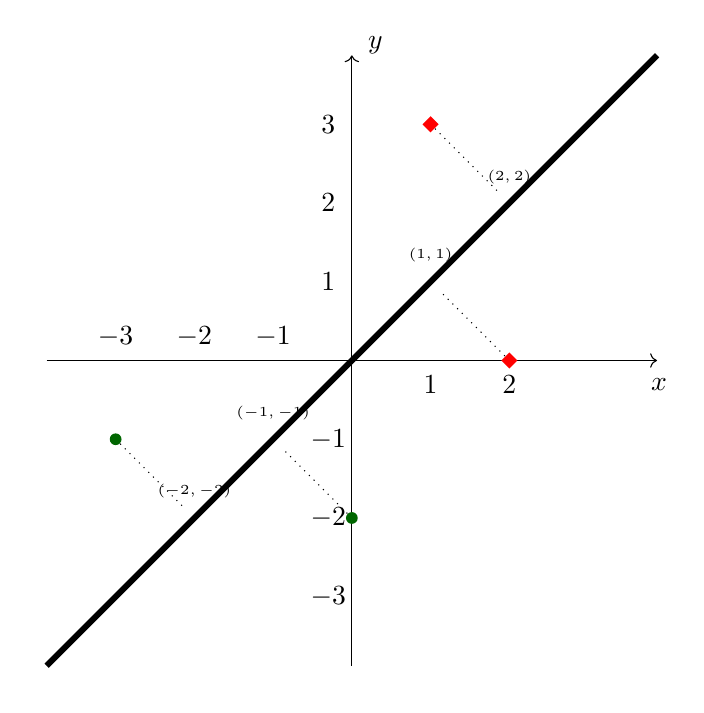
\begin{tikzpicture}
					\node (origin) at (0, 0) {};
					\node (top) at ($(origin) + (0, 4)$) {};
					\node (bottom) at ($(origin) + (0, -4)$) {};
					\node (left) at ($(origin) + (-4, 0)$) {};
					\node (right) at ($(origin) + (4, 0)$) {};
					\draw [->] (bottom) -- (top);
					\draw [->] (left) -- (right);
			
					\node at (-4, -4) (leftendpoint) {};
					\node at (4, 4) (rightendpoint) {};
					%\node at ($(origin) + (0.8, 1.3)$) {$y=\alpha x$};
					\node at ($(origin) + (3.9, -0.3)$) {$x$};
					\node at ($(origin) + (0.3, 4.0)$) {$y$};
			
					\draw[line width=0.75mm] (leftendpoint) -- (rightendpoint);
			
					\node[circle, fill=black!60!green, inner sep=1.5pt] at ($({-3/1.0}, {-1/1.0})$) (dp1) {};
					\node[circle, fill=black!60!green, inner sep=1.5pt] at ($({0/1.0}, {-2/1.0})$) (dp2) {};
					\node[diamond, fill=red, inner sep=1.5pt] at ($({2/1.0}, {0/1.0})$) (dp3) {};
					\node[diamond, fill=red, inner sep=1.5pt] at ($({1/1.0}, {3/1.0})$) (dp4) {};
					

					\node[label= {\tiny $\left( -2, -2\right)$}] at (-2, -2) (r1) {};
					\node[label= {\tiny $\left( -1, -1\right)$}] at (-1, -1) (r2) {};
					\node[label= {\tiny $\left( 1, 1\right)$}] at (1, 1) (r3) {};
					\node[label= {\tiny $\left( 2, 2\right)$}] at (2, 2) (r4) {};

					\draw[dotted] (dp1) -- (r1);
					\draw[dotted] (dp2) -- (r2);
					\draw[dotted] (dp3) -- (r3);
					\draw[dotted] (dp4) -- (r4);
			
					\node at ($({1/1.0}, 0.1)$) (dp1x) {};
					\node at ($(-0.1, {-2/1.0})$) (dp1y) {};
					\node at ($({1/1.0}, -0.3)$) {$1$};
					\node at ($(-0.3, {-2/1.0})$) {$-2$};
					%\draw[dotted] (dp1) -- (dp1x);
					%\draw[dotted] (dp1) -- (dp1y);
			
					\node at ($({2/1.0}, -0.1)$) (dp2x) {};
					\node at ($(-0.1, {3/1.0})$) (dp2y) {};
					\node at ($({2/1.0}, -0.3)$) {$2$};
					\node at ($(-0.3, {1/1.0})$) {$1$};
					\node at ($(-0.3, {2/1.0})$) {$2$};
					\node at ($(-0.3, {3/1.0})$) {$3$};
					%\draw[dotted] (dp2) -- (dp2x);
					%\draw[dotted] (dp2) -- (dp2y);
			
					\node at ($({-3/1.0}, 0.1)$) (dp3x) {};
					\node at ($(0.1, {-1/1.0})$) (dp3y) {};
					\node at ($({-3/1.0}, 0.3)$) {$-3$};
					\node at ($({-2/1.0}, 0.3)$) {$-2$};
					\node at ($({-1/1.0}, 0.3)$) {$-1$};
					\node at ($(-0.3, {-3/1.0} )$) {$-3$};
					\node at ($(-0.3, {-1/1.0} )$) {$-1$};
					%\draw[dotted] (dp3) -- (dp3x);
					%\draw[dotted] (dp3) -- (dp3y);
			
			
					\node[inner sep=0pt] at ($(leftendpoint)!(dp1)!(rightendpoint)$) (pdp1) {};
					\node[inner sep=0pt] at ($(leftendpoint)!(dp2)!(rightendpoint)$) (pdp2) {};
					\node[inner sep=0pt] at ($(leftendpoint)!(dp3)!(rightendpoint)$) (pdp3) {};
			
					%\draw[red] (dp1) -- (pdp1);
					%\draw[red] (dp2) -- (pdp2);
					%\draw[red] (dp3) -- (pdp3);
				\end{tikzpicture}
\end{Described}
				\caption{Plot of Transactions in 2-D}
			\end{figure}
		}


\end{enumerate}

  \newpage
  \qns{Diode System ID (Adapted from EECS 16B Fall 2023 Final)}

    \textbf{Note: This problem does not require knowledge of circuits or diodes.}
    
    Suppose that we want to characterize a diode $D_1$ with parasitic resistance $R_p$, represented by the following model:
    \begin{figure}[H]
        \begin{center}
            \begin{Described}{Voltage source V sub B drives from ground up to the top node, where diode D1 carries current I D to the right with voltage V D across it, in series with resistor R sub p returning to ground.}
\begin{circuitikz}
                \draw (0, 2) to [V, l_=$V_B$] (0, 0) node[ground]{}
                (0, 2) to [Do, l=$D_1$, i=$I_D$, v=$V_D$] (3, 2) to [R, l=$R_p$] (5, 2) node[ground]{}
                ;
            \end{circuitikz}
\end{Described}
        \end{center}
    \end{figure}
    The current through the diode (forward-biased) is modeled as
    \begin{equation}
        I_D = I_0\e^{\frac{V_D}{V_T}}
    \end{equation}
    where $V_D$ is the voltage across the diode (as shown in the diagram), $I_0$ is a parameter associated with the diode, and $V_T$ is the thermal voltage, a temperature dependent variable.
    
    With some analysis, the system equation can be simplified to:
    \begin{equation}
        I_D = I_0 \e^{\frac{V_B - I_D R_p}{V_T}}
    \end{equation}
    To collect data, we will vary the temperature to vary $V_T$ and measure the current $I_D$ through the diode.
    
        \begin{enumerate}

            \qitem    Use the provided system equation to show that
                \begin{equation}
                    I_D R_p - V_T \ln(I_0) = V_B - V_T \ln(I_D)
                \end{equation}
                    is a valid equation to represent the system.
                \begin{hint}
                    Use the logarithm identity $\ln(\frac{a}{b}) = \ln(a) - \ln(b)$.
                \end{hint}
            
    
            \ans{
                \begin{align}
                    I_D &= I_0 \e^{\frac{V_B - I_D R_p}{V_T}} \\
                    V_T\ln(\frac{I_D}{I_0}) &= V_B - I_D R_p \\
                    V_T\ln(I_D) - V_T\ln(I_0) &= V_B - I_D R_p \\
                    I_D R_p - V_T \ln(I_0) &= V_B - V_T \ln(I_D)
                \end{align}
            }
    
            % \begin{problempart}{4}{System ID}{0}{0}
            %     Suppose we use $V_B = 1 \mathrm{V}$ and collect the following data points:
            %     \begin{itemize}
            %         \item For $V_T = 0.025 \mathrm{V}$, $I_D = 0.0185 \mathrm{A}$.
            %         \item For $V_T = 0.05 \mathrm{V}$, $I_D = 0.0172 \mathrm{A}$.
            %         \item For $V_T = 0.0125 \mathrm{V}$, $I_D = 0.0193 \mathrm{A}$.
            %     \end{itemize}
            %     \textbf{Find the matrix $D$ and vector $\vec{s}$ to set up a least-squares problem $D\vec{p} \approx \vec{s}$ where $\vec{p} = \begin{bmatrix} \ln(I_0) \\ R_p \end{bmatrix}$.}
    
            %     You do not have to simplify the elements $D$ and $\vec{s}$, but the elements should be numerical values, not in terms of variables.
            % \end{problempart}
    
            % \begin{solution}{4in}
            %     Each data point can be used with the provided system equation from the first part to create a system of linear equations with the unknowns being $\ln(I_0)$ and $R_p$ (remember that the problem provides that $V_B = 1 \mathrm{V}$):
            %     \begin{itemize}
            %         \item $-0.025\ln(I_0) + 0.0185R_p = 1 - 0.025\ln(0.0185)$
            %         \item $-0.05\ln(I_0) + 0.0172R_p = 1 - 0.05\ln(0.0172)$
            %         \item $-0.0125\ln(I_0) + 0.0193R_p = 1 - 0.0125\ln(0.0193)$
            %     \end{itemize}
            %     The matrix form of this system is:
            %     \begin{equation}
            %         \begin{bmatrix} -0.025 & 0.0185 \\ -0.05 & 0.0172 \\ -0.0125 & 0.0193 \end{bmatrix} \begin{bmatrix} \ln(I_0) \\ R_p \end{bmatrix} = \begin{bmatrix} 1 - 0.025\ln(0.0185) \\ 1 - 0.05\ln(0.0172) \\ 1 - 0.0125\ln(0.0193) \end{bmatrix}
            %     \end{equation}
            %     Thus, for the least-squares problem, $D = \begin{bmatrix} -0.025 & 0.0185 \\ -0.05 & 0.0172 \\ -0.0125 & 0.0193 \end{bmatrix}$ and $\vec{s} = \begin{bmatrix} 1 - 0.025\ln(0.0185) \\ 1 - 0.05\ln(0.0172) \\ 1 - 0.0125\ln(0.0193) \end{bmatrix}$
            % \end{solution}
    
            \vspace{5cm}
            
            \qitem    Suppose we use $V_B = v_B$ and collect the following data points:
                \begin{itemize}
                    \item For $V_T = v_{T1}$, $I_D = i_{D1}$.
                    \item For $V_T = v_{T2}$, $I_D = i_{D2}$.
                    \item For $V_T = v_{T3}$, $I_D = i_{D3}$.
                \end{itemize}
                Find the matrix $\textbf{A}$ and vector $\vec{x}$ to set up a least-squares problem $\textbf{A} \vec{x} \approx \vec{b}$ where $\vec{x} = \begin{bmatrix} \ln(I_0) \\ R_p \end{bmatrix}$
    
            \ans{
                Each data point can be used with the provided system equation from the first part to create a system of linear equations with the unknowns being $\ln(I_0)$ and $R_p$ (remember that the problem provides that $V_B = v_B$):
                \begin{itemize}
                    \item $-v_{T1}\ln(I_0) + i_{D1}R_p = v_B - v_{T1}\ln(i_{D1})$
                    \item $-v_{T2}\ln(I_0) + i_{D2}R_p = v_B - v_{T2}\ln(i_{D2})$
                    \item $-v_{T3}\ln(I_0) + i_{D3}R_p = v_B - v_{T3}\ln(i_{D3})$
                \end{itemize}
                The matrix form of this system is:
                \begin{equation}
                    \begin{bmatrix} -v_{T1} & i_{D1} \\ -v_{T2} & i_{D2} \\ -v_{T3} & i_{D3} \end{bmatrix} \begin{bmatrix} \ln(I_0) \\ R_p \end{bmatrix} = \begin{bmatrix} v_B - v_{T1}\ln(i_{D1}) \\ v_B - v_{T2}\ln(i_{D2}) \\ v_B - v_{T3}\ln(i_{D3}) \end{bmatrix}
                \end{equation}
                Thus, for the least-squares problem, $\textbf{A} = \begin{bmatrix} -v_{T1} & i_{D1} \\ -v_{T2} & i_{D2} \\ -v_{T3} & i_{D3} \end{bmatrix}$ and $\vec{b} = \begin{bmatrix} v_B - v_{T1}\ln(i_{D1}) \\ v_B - v_{T2}\ln(i_{D2}) \\ v_B - v_{T3}\ln(i_{D3}) \end{bmatrix}$
            }
            
            \vspace{5cm}
            
            \qitem    Explain how you would use the least-squares system from the previous part to find model parameters $I_0$ and $R_p$. You do not need to use actual values for this part; you explanation can just use $\textbf{A}$ and $\vec{b}$ as known variables to show what calculations you would do to find $I_0$ and $R_p$.
            
    
            \ans{
                We would first find the optimal parameter $\hat{\vec{x}}$ with the least squares formula:
                \begin{equation}
                    \hat{\vec{x}} = (\textbf{A}^\top \textbf{A})^{-1} \textbf{A}^{\top} \vec{b}
                \end{equation}
                The elements of $\hat{\vec{x}}$ represent optimal values for $\ln(I_0)$ and $R_p$ so we set the elements of $\hat{\vec{x}}$ equal to those parameters for our model:
                \begin{align}
                    \hat{x}_{v_B} = \ln(I_0) &\rightarrow I_0 = \e^{\hat{x}_1} \\
                    \hat{x}_2 = R_p &\rightarrow R_p = \hat{x}_2
                \end{align}
                Thus, we have found parameter values for $I_0$ and $R_p$ from the least-squares system.
            }
    
        \end{enumerate}

\end{qunlist}

\end{document}
"

\DocumentMetadata{
  lang       = en-US,
  pdfversion = 2.0,
  testphase  = {phase-III,math,table,graphic,firstaid},
}
\documentclass{latexally-assignment}

\usepackage{amsmath,amssymb}
\usepackage{float}
\usepackage{tikz}
\usetikzlibrary{calc,shapes.geometric,positioning}
\usepackage[american]{circuitikz}

% The corpus macros these four files use, reproduced from questionBank/ee16.sty
% and questionBank/sp26/sp26.sty so the demo does not need the whole course
% preamble chain. Same meanings, nothing more.
\providecommand{\bmqty}[1]{\begin{bmatrix}#1\end{bmatrix}}
\providecommand{\e}{\mathop{\mathrm{e}}\nolimits}
\providecommand{\wt}[1]{\widetilde{#1}}
\NewDocumentEnvironment{hint}{+b}{\itshape (HINT: #1)}{}

\setcoursenumber{EECS 16A}
\setcoursename{Designing Information Devices and Systems I}
\setsemester{Spring 2026}

\begin{document}

\def\title{Described figures from the question bank}
\maketitle

\vspace{0.5em}
Every figure below carries a description in the PDF structure tree. A screen
reader announces "graphic" and then that description; it never reaches the
drawing underneath. Hovering shows nothing --- \texttt{/Alt} is not a tooltip.

\begin{qunlist}

  \qns{Polynomial Multiplication and Discrete-Time Convolution [Adapted from EE 120]}
% Adapted and extended by Ken Zheng for EECS 16A Fall 2025 Discussion

The impulse response of a real, discrete-time FIR filter $\mathsf{A}$ is described by  
$$a[n]=a_0 \delta[n]+a_1 \delta[n-1]+\cdots + a_N \delta[n-N], \quad \text{where } N\in \{1,2,3,\ldots\}.$$

\begin{enumerate}[(a)]
\item Show that the frequency response $A(\omega)$ of the filter is a polynomial, in terms of $e^{-i\omega}$, whose coefficients have a simple relationship with the impulse response values $a_0,\ldots,a_N$.

\ans{

    Substituting \(a[n]\) into the frequency response formula we see that:
    \begin{equation*}
        A(w) = \sum_{n=-\infty}^{\infty} a[n]e^{-iwn}
    \end{equation*}
    As $a[n] = 0$ outside the range of $n = 0$ to $n = N$ ,
    \begin{equation*}
        A(w) = a_0 e^{-iw\cdot 0} + a_1 e^{-iw\cdot 1} + \ldots + a_N e^{-iw\cdot N}
    \end{equation*}
    \begin{equation*}
        = a_0 + a_1 e^{-iw} + \ldots + a_N e^{-iwN}
    \end{equation*}
}
\item Suppose the filter $\mathsf{A}$ is placed in a cascade (series) interconnection with another discrete-time FIR filter $\mathsf{B}$ whose impulse response is described by  
$$b[n]=b_0 \delta[n]+b_1 \delta[n-1]+\cdots + b_M \delta[n-M],\quad \text{where } M\in \{1,2,3,\ldots\}.$$

The cascade structure, which we call $\mathsf{C}$, is shown in the figure below.
\vspace{4pt}

\centerline{
    \begin{Described}{Block diagram: input x enters block A, whose output feeds block B, and block B's output is y. An outer box enclosing both blocks is labelled C.}
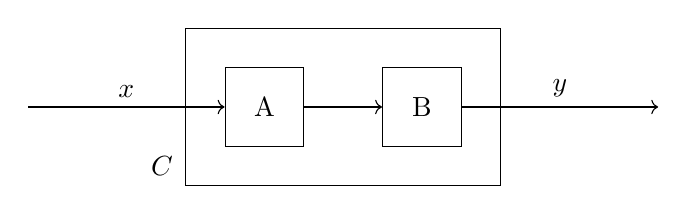
\begin{tikzpicture}
        % Define nodes for blocks A and B
        \node[draw, rectangle, minimum width=1cm, minimum height=1cm] (A) at (0,0) {A};
        \node[draw, rectangle, minimum width=1cm, minimum height=1cm] (B) at (2,0) {B};
        
        % Draw the outer rectangle
        \draw (-1, 1) rectangle (3, -1);
        
        % Draw arrows and labels
        \draw[->] (-3, 0) -- (A.west) node[midway,above] {$x$};
        \draw[->] (A.east) -- (B.west);
        \draw[->] (B.east) -- (5, 0) node[midway,above] {$y$};
        
        % Label C 
        \node at (-1.3, -0.5) [below] {$C$};
    \end{tikzpicture}
\end{Described}
}
Let $c$ denote the impulse response of the cascade interconnection.

\begin{enumerate}[(i)]
\item Express $c$ in terms of $a$ and $b$.
    
\ans{

        The impulse response \(c\) of the cascade interconnection is given by 
        \begin{equation*}
            c[n] = (a * b)[n] = \sum_{k=-\infty}^{\infty} a[k]\,b[n-k]
        \end{equation*}
         Substituting \(n = 0\):
        \begin{equation*}
            c_0 = a_0 b_0
        \end{equation*}
        \(n = 1\):
        \begin{equation*}
            c_1 = a_0 b_1 + a_1 b_0 
        \end{equation*}
        \(n = 2\):
        \begin{equation*}
            c_2 = a_0 b_2 + a_1 b_1 + a_2 b_0
        \end{equation*}
        And so on...
    
        Thus, we can write:
        \begin{equation*}
            c_n = \sum_{k=\max(0,n-M)}^{\min(n, N)} a_k b_{n-k}
        \end{equation*}
        \null\hfill for \(n = 0, 1, \ldots, N + M\)
        
        where we found the bounds of summation from the two conditions that ensure we are indexing \(a[n]\) and \(b[n]\) without exceeding the bounds of their signal.
        $$ 0 \leq k \leq N \Longrightarrow k \leq N \quad \text{and} \quad k \geq 0 $$
        $$ 0 \leq n - k \leq M \Longrightarrow k \leq n \quad \text{and} \quad k \geq n - M $$
        and so
        $$ k \leq \min(n, N) \quad \text{and} \quad k \geq \max(0, n-M) $$

        Lastly, 
         \begin{equation*}
            c[n] = c_0\delta[n] + c_1 \delta[n - 1] + ... + c_{N + M} \delta[n - ( N + M)]
        \end{equation*}
        
    }

\item Consider two polynomials $A(z)$ and $B(z)$ described as follows:
    $$
    A(z) = a_0 +a_1 z + \cdots + a_N z^N \quad \quad \quad B(z) = b_0 +b_1 z + \cdots + b_M z^M \, ,
    $$
    where $M$ and $N$ and positive integers.
    Let $C(z)=A(z)\, B(z)$, where $$ C(z) = c_0 +c_1 z + \cdots + c_{N+M} z^{N+M}.$$  Show that multiplying polynomials is tantamount to convolving their coefficients; in particular, explain how $c_n=(a*b)_n=\displaystyle\sum_m a_m b_{n-m}$, where $n={0,1,\ldots, N+M}$.
    
    \ans{
    \begin{equation*}
        C(z) = (a_0 +a_1 z + \cdots + a_N z^N) (b_0 +b_1 z + \cdots + b_M z^M)
    \end{equation*}
    \begin{equation*}
        C(z) = a_0 b_0 + (a_0 b_1 + a_1 b_0) z + (a_0 b_2 + a_1 b_1 + a_2 b_0) z^2 + ...
    \end{equation*}
    As you can see, each coefficient of \(z^n\) is the sum of all products of \(a_i\) and \(b_j\) where \(i + j = n\):
    \begin{equation*}
        c_n =  \sum_{m=\max(0,n-M)}^{\min(n, N)} a_m b_{n-m}
    \end{equation*}
    \null\hfill for \(n = 0, 1, 2, ..., N + M\)

    Just like the definition of convolution!
    }

\end{enumerate}
\end{enumerate}
  \newpage
  \qns{Frequency Response from a DAG Block Diagram [Adapted from EE 120]}
% Adapted by Ken Zheng for EECS 16A Fall 2025 Discussion

    Consider a DT LTI system with input $x[n]$ and output $y[n]$ that is implemented by the following block diagram:
    \begin{figure}[h!]
      \centering
      \begin{Described}{Block diagram: input x of n enters a summing junction whose output is y of n. That output is tapped, passed through a delay block D and then a gain of minus 0.5, and fed back into the summing junction.}
\begin{circuitikz}
          \node (x) at (0, 0) {$x[n]$};
          \node[circle, draw] (sum) at (2, 0) {$+$};
          % FIXME: find a better way to draw the triangle
          % \node[triangleblock, shape border rotate=90, inner sep=-1mm] (gain) at (3, -1.5) {$-0.5$};
          % \node at (3, -1.5) {$-0.5$};
          \node[draw, inner sep=5pt] (delay) at (6, -1.5) {$D$};
          \node (y) at (9, 0) {$y[n]$};
          \draw[->] (x.east) -- (sum.west);
          \draw[->] (sum.east) -- (y.west);
          \draw[->] (7.5, 0) -- (7.5, -1.5) -- (delay.east);
          % \draw[-, thick] (delay.west) -- (gain.east);
          % \draw[->, thick] (gain.west) -- (2, -1.5) -- (sum.south);
          \draw[->] (delay.west) to [amp, t=$-0.5$, blocks/scale=1.5] (2, -1.5) to (sum.south);
      \end{circuitikz}
\end{Described}
  \end{figure}
\begin{enumerate}
        \item Find the LCCDE that describes this system. 
        
        \ans{
            The difference equation describing this system is
              \begin{equation*}
                y[n] = x[n] - 0.5y[n-1]
              \end{equation*}
        }

        \item Find the frequency response $H(\omega)$ of this system. 
            
        \ans{
            Using the eigenfunction property by setting $x[n] = e^{i\omega n}$ and $y[n] = H(\omega) e^{i\omega n}$,
            \begin{align*}
            H(\omega) e^{i\omega n} &= e^{i\omega n} - 0.5 H(\omega) e^{i\omega (n-1)} \\
            &= e^{i\omega n} - 0.5 H(\omega) e^{-i\omega}e^{i\omega n} \\
            \left(1 + 0.5 e^{-i\omega}\right) e^{i\omega n} H(\omega) &= e^{i\omega n} \\
            H(\omega) &= \frac{e^{i\omega n}}{\left(1 + 0.5 e^{-i\omega}\right)e^{i\omega n}} \\
                &= \frac{1}{1 + 0.5 e^{-i\omega}}
            \end{align*} 
        } 

        \vspace{4cm}

        \item Is this a high pass or low pass filter?
        
        \ans{
            We can think about this in two ways:
            
            \textbf{1. Geometric Approach:}

            Recall from part (b) that the frequency response can be written as:
            \[
            H(\omega) = \frac{1}{1 + 0.5 e^{-i\omega}} = \frac{e^{i\omega}}{e^{i\omega} - (-0.5)}
            \]
            The magnitude is therefore:
            \[
            |H(\omega)| = \frac{1}{|e^{i\omega} - (-0.5)|}
            \]
            This represents the reciprocal of the distance from the point $e^{i\omega}$ on the unit circle to the point located at $-0.5$ on the real axis:

            \begin{center}
            \begin{Described}{Complex plane with real and imaginary axes and the unit circle centred at the origin. A point is marked at minus 0.5 on the real axis, with an arrow from it to the point e to the i omega on the circle.}
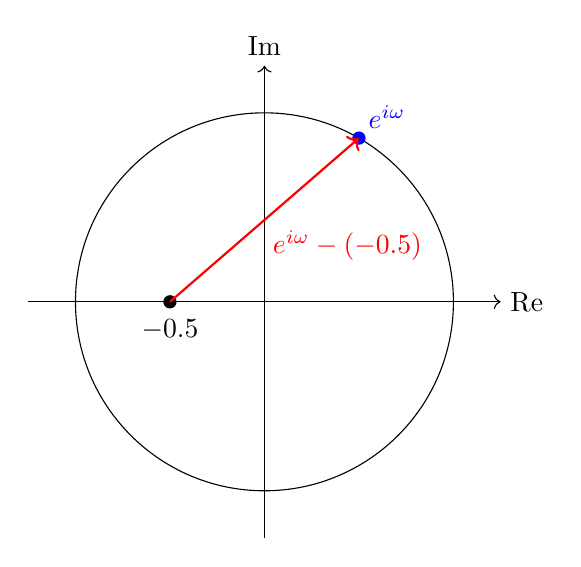
\begin{tikzpicture}[scale=1.2]
                % Axes
                \draw[->] (-2.5,0) -- (2.5,0) node[right] {$\operatorname{Re}$};
                \draw[->] (0,-2.5) -- (0,2.5) node[above] {$\operatorname{Im}$};

                % Unit circle
                \draw (0,0) circle (2);

                % Pole at -0.5
                \fill[black] (-1,0) circle (2pt) node[below left] {};
                \node[black] at (-1,-0.3) {$-0.5$};

                % Point on unit circle at angle ω
                \coordinate (P) at (60:2);
                \fill[blue] (P) circle (2pt) node[above right] {$e^{i\omega}$};

                % Vector from pole to point on circle
                % \draw[->, thick, red] (-1,0) -- (P);
                \draw[->, thick, red] (-1,0) -- (P) node[midway, below] {$\qquad\qquad\qquad e^{i \omega} - (-0.5)$};  % Label added here


                % Labels
                \node at (1.8,1.8) {};
            \end{tikzpicture}
\end{Described}
            \end{center}

            Key observations:
            \begin{itemize}
                \item When $\omega = 0$, $e^{i\omega} = 1$. The distance from $1$ to $-0.5$ is $1.5$, so $|H(0)| = 1/1.5 \approx 0.667$.
                \item When $\omega = \pi$, $e^{i\omega} = -1$. The distance from $-1$ to $-0.5$ is $0.5$, so $|H(\pi)| = 1/0.5 = 2$.
                \item As $\omega$ moves from $0$ to $\pi$, the point $e^{i\omega}$ travels along the upper half of the unit circle from $(1,0)$ to $(-1,0)$. 
                The distance to the point at $-0.5$ decreases monotonically, so $|H(\omega)|$ increases. Thus, we have a high-pass filter!\\
            \end{itemize}

            
            \textbf{2. Algebraic Approach:}
            
            To determine the filter type, we simplify the magnitude of the frequency response first:

            \[
            |H(\omega)| = \frac{1}{\sqrt{(1 + 0.5\cos\omega)^2 + (0.5\sin\omega)^2}}
            \]


            Expanding \( (1 + 0.5\cos\omega)^2 \) and \( (0.5\sin\omega)^2 \):
            \[
            (1 + 0.5\cos\omega)^2 = 1^2 + 2(1)(0.5\cos\omega) + (0.5\cos\omega)^2 = 1 + \cos\omega + 0.25\cos^2\omega
            \]
            \[
            (0.5\sin\omega)^2 = 0.25\sin^2\omega
            \]


            Add the two results in the square root:
            \[
            (1 + 0.5\cos\omega)^2 + (0.5\sin\omega)^2 = \left[1 + \cos\omega + 0.25\cos^2\omega\right] + \left[0.25\sin^2\omega\right]
            \]
            \[
            = 1 + \cos\omega + 0.25\left(\cos^2\omega + \sin^2\omega\right)
            \]
            \[
            = 1 + \cos\omega + 0.25(1) = 1 + \cos\omega + 0.25 = 1.25 + \cos\omega
            \]


            Substitute back into \( |H(\omega)| \):
            \[
            |H(\omega)| = \frac{1}{\sqrt{1.25 + \cos\omega}}
            \]
                        
            Now we analyze the magnitude at key frequencies:
            
            Low frequency (\( \omega = 0 \)): 
                \[
                |H(0)| =  \frac{1}{\sqrt{1.25 + \cos0}} = \frac{1}{1.5} \approx 0.667 \quad (\text{attenuated})
                \]
            High frequency (\( \omega = \pi \)): 
                \[
                |H(\pi)| =  \frac{1}{\sqrt{1.25 + \cos\pi}} = 2 \quad (\text{passed})
                \]

            We can see that, again, the filter attenuates low frequencies and passes high frequencies, so it is a high-pass filter!\\

            Both geometrically and algebraically, we conclude this is a \textbf{high-pass filter}. Nice!
        }
\end{enumerate}

  \newpage
  \qns{Using PCA to Detect Fraudulent Transactions (Adapted from EECS 16B Spring 2023 Final)}\\
	PCA has many different uses when applied to real-world data. One potential application is making classification of data much easier.
	
	Suppose we are given some data, where each datapoint represents a transaction. Each one is labeled either normal or fraudulent. We will utilize PCA to develop a useful classifier.

	We plot the data in two dimensions, where each dimension is some unspecified feature that will aid us in classifying the points:

	\begin{figure}[H]
        \centering
        \begin{Described}{Scatter plot on x and y axes running about minus 4 to 4, with four transactions marked: circles at (-3, -1) and (0, -2), and diamonds at (2, 0) and (1, 3).}
\begin{tikzpicture}
            \node (origin) at (0, 0) {};
            \node (top) at ($(origin) + (0, 4)$) {};
            \node (bottom) at ($(origin) + (0, -4)$) {};
            \node (left) at ($(origin) + (-4, 0)$) {};
            \node (right) at ($(origin) + (4, 0)$) {};
            \draw [->] (bottom) -- (top);
            \draw [->] (left) -- (right);
    
            \node at (-3, -2.2) (leftendpoint) {};
            \node at (3, 2.2) (rightendpoint) {};
            %\node at ($(origin) + (0.8, 1.3)$) {$y=\alpha x$};
            \node at ($(origin) + (3.9, -0.3)$) {$x$};
            \node at ($(origin) + (0.3, 4.0)$) {$y$};
    
            %\draw[line width=0.75mm] (leftendpoint) -- (rightendpoint);
    
            \node[circle, fill=black!60!green, inner sep=1.5pt] at ($({-3/1.0}, {-1/1.0})$) (dp1) {};
            \node[circle, fill=black!60!green, inner sep=1.5pt] at ($({0/1.0}, {-2/1.0})$) (dp2) {};
            \node[diamond, fill=red, inner sep=1.5pt] at ($({1/1.0}, {3/1.0})$) (dp3) {};
			\node[diamond, fill=red, inner sep=1.5pt] at ($({2/1.0}, {0/1.0})$) (dp4) {};
    
            \node at ($({1/1.0}, 0.1)$) (dp1x) {};
            \node at ($(-0.1, {-2/1.0})$) (dp1y) {};
            \node at ($({1/1.0}, 0.3)$) {$1$};
            \node at ($(-0.3, {-2/1.0})$) {$-2$};
            %\draw[dotted] (dp1) -- (dp1x);
            %\draw[dotted] (dp1) -- (dp1y);
    
            \node at ($({2/1.0}, -0.1)$) (dp2x) {};
            \node at ($(-0.1, {3/1.0})$) (dp2y) {};
            \node at ($({2/1.0}, -0.3)$) {$2$};
            \node at ($(-0.3, {3/1.0})$) {$3$};
            %\draw[dotted] (dp2) -- (dp2x);
            %\draw[dotted] (dp2) -- (dp2y);
    
            \node at ($({-3/1.0}, 0.1)$) (dp3x) {};
            \node at ($(0.1, {-1/1.0})$) (dp3y) {};
            \node at ($({-3/1.0}, 0.3)$) {$-3$};
            \node at ($(-0.3, {-1/1.0 -0.3} )$) {$-1$};
            %\draw[dotted] (dp3) -- (dp3x);
            %\draw[dotted] (dp3) -- (dp3y);
    
    
            \node[inner sep=0pt] at ($(leftendpoint)!(dp1)!(rightendpoint)$) (pdp1) {};
            \node[inner sep=0pt] at ($(leftendpoint)!(dp2)!(rightendpoint)$) (pdp2) {};
            \node[inner sep=0pt] at ($(leftendpoint)!(dp3)!(rightendpoint)$) (pdp3) {};
    
            %\draw[red] (dp1) -- (pdp1);
            %\draw[red] (dp2) -- (pdp2);
            %\draw[red] (dp3) -- (pdp3);
        \end{tikzpicture}
\end{Described}
        \caption{Plot of Transactions in 2-D}
	\end{figure}

	Thus, we have a total of 4 transactions, $\bmqty{-3 \\ -1}$ and $\bmqty{0 \\ -2}$ are normal, while $\bmqty{2 \\ 0}$ and $\bmqty{1 \\ 3}$ are fraudulent.
	\begin{enumerate}
		%Part A:
		
		\qitem Suppose we now construct a data matrix, where the \textit{data points are columns}. 

			\begin{equation}
				X = \bmqty{-3 & 0 & 2 & 1 \\ -1 & -2 & 0 & 3}
			\end{equation}

			Using this data matrix, \textbf{calculate its first principal component $\vec{u}_1$}.

			\begin{hint}
			\begin{enumerate}

				\item You may also make use of the fact that $XX^T$ is given by:
				\begin{align}
					XX^{\top} &= \bmqty{-3 & 0 & 2 & 1 \\ -1 & -2 & 0 & 3}\bmqty{-3 & 0 & 2 & 1 \\ -1 & -2 & 0 & 3}^{\top} \\
						&= \bmqty{14 & 6 \\ 6 & 14}
				\end{align}
				\item You may also make use of the characteristic polynomial of $XX^T$:
				\begin{equation}
					\lambda^2 - 28\lambda + 160 = (\lambda - 20)(\lambda - 8) = 0
				\end{equation}
			\end{enumerate}
			\end{hint}
			
			\begin{hint} Remember that your principal component should be of unit norm. \end{hint}

		\ans{
			% From PCA, we know that our first principal component of a matrix with column data is the first column vector of $U$ in the SVD of $X$. Thus, we use the SVD method of calculation (find the eigenvector corresponding to the largest eigenvalue of $XX^{\top}$ and normalize to yield $\vec{u}_1$).

			% \begin{align}
			% 	XX^{\top} &= \bmqty{-3 & 0 & 2 & 1 \\ -1 & -2 & 0 & 3}\bmqty{-3 & 0 & 2 & 1 \\ -1 & -2 & 0 & 3}^{\top} \\
			% 		 &= \bmqty{14 & 6 \\ 6 & 14}
			% \end{align}

			% From setting $\mathrm{det}(XX^{\top} - \lambda I) = 0$, we should find our characteristic polynomial to be 
			
			% \begin{equation}
			% 	\lambda^2 - 28\lambda + 160 = 0
			% \end{equation}

			Our eigenvalues are $\lambda_1 = 20$ and $\lambda_2 = 8$. Thus, the eigenvector corresponding to our largest eigenvalue $\lambda_1 = 20$ is $\vec{v}_1 = \bmqty{1 \\ 1}$ from inspection.
			
			Thus, our principal component vector is given as the normalized eigenvector: i.e. $\vec{u}_1 = \bmqty{\frac{1}{\sqrt{2}} \\ \frac{1}{\sqrt{2}}}$.
        }

		%Part B:
		
		\qitem	It's difficult to come up with a useful classifier in two dimensions. Let's use PCA dimensionality reduction to help.
			
			Using your answer in part (a), \textbf{project your two-dimensional data points onto one dimension. Express your answer as the vector $\vec{z} \in \mathbb{R}^{1 \times 4}$.}

		\ans{
			To project our 2-d data into 1-d, we project our data matrix onto the first principal component as follows:
			
			\begin{equation}
				\vec{z} = \vec{u}_1^{\top}X = \bmqty{\frac{1}{\sqrt{2}} \\ \frac{1}{\sqrt{2}}} \bmqty{-3 & 0 & 2 & 1 \\ -1 & -2 & 0 & 3} = \bmqty{-\frac{4}{\sqrt{2}} & -\frac{2}{\sqrt{2}} & \frac{2}{\sqrt{2}} & \frac{4}{\sqrt{2}}}
			\end{equation}
		}
		
		%Part C:
		
		\qitem	Now, plot each of these points, on the line below. Indicate the value and label (normal as circle and fraudulent as diamond) for each point.
			
			\textit{Note: your plot doesn't have to be to scale.}

			\begin{figure}[H]
				\centering
				\begin{Described}{Blank horizontal number line labelled z, with only the origin marked 0 and no points plotted.}
\begin{tikzpicture}
					\node (origin) at (0, 0) {|};
            		%\node (top) at ($(origin) + (0, 4)$) {};
            		%\node (bottom) at ($(origin) + (0, -4)$) {};
            		\node (left) at ($(origin) + (-4, 0)$) {};
            		\node (right) at ($(origin) + (4, 0)$) {};
					\node at ($(origin) + (3.9, -0.3)$) {$z$};
					\node at ($(origin) + (0, -0.3)$) {0};
            		%\draw [->] (bottom) -- (top);
            		\draw [<->] (left) -- (right);

				\end{tikzpicture}
\end{Described}
				\caption{Plot of Transactions in 1-D}
			\end{figure}

		\ans{
			\begin{figure}[H]
				\centering
				\begin{Described}{Number line labelled z with the origin marked 0 and four points: circles at minus four over root two and minus two over root two, diamonds at two over root two and four over root two.}
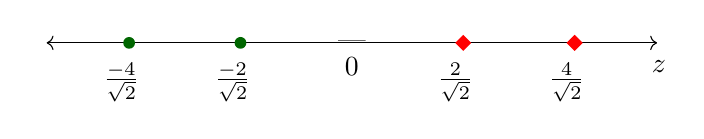
\begin{tikzpicture}
					\node (origin) at (0, 0) {|};
            		%\node (top) at ($(origin) + (0, 4)$) {};
            		%\node (bottom) at ($(origin) + (0, -4)$) {};
            		\node (left) at ($(origin) + (-4, 0)$) {};
            		\node (right) at ($(origin) + (4, 0)$) {};
					\node at ($(origin) + (3.9, -0.3)$) {$z$};
					\node at ($(origin) + (0, -0.3)$) {0};
            		%\draw [->] (bottom) -- (top);
            		\draw [<->] (left) -- (right);

					\node[circle, fill=black!60!green, inner sep=1.5pt] at ($(origin) + (-4/1.414, 0)$) (dp1) {};
					\node at ($(origin) + (-4/1.414 -0.1, -0.5)$) {$\frac{-4}{\sqrt{2}}$};
					\node[circle, fill=black!60!green, inner sep=1.5pt] at ($(origin) + (-2/1.414, 0)$) (dp1) {};
					\node at ($(origin) + (-2/1.414 -0.1, -0.5)$) {$\frac{-2}{\sqrt{2}}$};
					\node[diamond, fill=red, inner sep=1.5pt] at ($(origin) + (2/1.414, 0)$) (dp1) {};
					\node at ($(origin) + (2/1.414 -0.1, -0.5)$) {$\frac{2}{\sqrt{2}}$};
					\node[diamond, fill=red, inner sep=1.5pt] at ($(origin) + (4/1.414, 0)$) (dp1) {};
					\node at ($(origin) + (4/1.414 -0.1, -0.5)$) {$\frac{4}{\sqrt{2}}$};
				\end{tikzpicture}
\end{Described}
				\caption{Plot of Transactions in 1-D}
			\end{figure}
		}

		%Part D:
		
		\qitem	Suppose you are given some transaction datapoint, $\vec{x}_i$ and you project it to be one-dimensional, i.e. $z_i$. \textbf{Based on your plot from part (c), come up with an inequality in terms of $z_i$ to identify if that transaction is fraudulent.}
			
			\textit{Note: There can be more than one answer, but please only give one.}

		\ans{
			$\vec{z}_i > 0$ is a possible answer. In fact any answer in between $\vec{z}_i \geq -\frac{2}{\sqrt{2}}$ and $\vec{z}_i \geq \frac{2}{\sqrt{2}}$ is valid.
		}

		%Part E:
		
		\qitem	It can often be informative to compare our original data with its PCA reconstructions. \textbf{Using PCA, reconstruct $\vec{z}$ back into 2-D as the matrix $\wt{X} \in \mathbb{R}^{2 \times 4}$.}

		\ans{
			Using the reconstruction principle of PCA, we lift the 1D data back into 2 dimensions by doing the following:
			\begin{equation}
				\wt{X} = \vec{u}_1\vec{u}_1^{\top}X = \bmqty{-2 & -1 & 1 & 2 \\ -2 & -1 & 1 & 2}
			\end{equation}
		}

		%Part F:
		
		\qitem	Finally, we visualize our PCA reconstruction. \textbf{On the graph below, draw your first principal component direction (extend it as a solid line in both directions). Draw your reconstructioned points from $\wt{X}$, with dotted lines connecting them with the corresponding point in $X$. } You may draw on the plot on the next page.

			\begin{figure}[H]
				\centering
				\begin{Described}{Scatter plot on x and y axes running about minus 4 to 4, with four transactions marked: circles at (-3, -1) and (0, -2), and diamonds at (2, 0) and (1, 3).}
\begin{tikzpicture}
					\node (origin) at (0, 0) {};
					\node (top) at ($(origin) + (0, 4)$) {};
					\node (bottom) at ($(origin) + (0, -4)$) {};
					\node (left) at ($(origin) + (-4, 0)$) {};
					\node (right) at ($(origin) + (4, 0)$) {};
					\draw [->] (bottom) -- (top);
					\draw [->] (left) -- (right);
			
					\node at (-3, -2.2) (leftendpoint) {};
					\node at (3, 2.2) (rightendpoint) {};
					%\node at ($(origin) + (0.8, 1.3)$) {$y=\alpha x$};
					\node at ($(origin) + (3.9, -0.3)$) {$x$};
					\node at ($(origin) + (0.3, 4.0)$) {$y$};
			
					%\draw[line width=0.75mm] (leftendpoint) -- (rightendpoint);
			
					\node[circle, fill=black!60!green, inner sep=1.5pt] at ($({-3/1.0}, {-1/1.0})$) (dp1) {};
					\node[circle, fill=black!60!green, inner sep=1.5pt] at ($({0/1.0}, {-2/1.0})$) (dp2) {};
					\node[diamond, fill=red, inner sep=1.5pt] at ($({1/1.0}, {3/1.0})$) (dp3) {};
					\node[diamond, fill=red, inner sep=1.5pt] at ($({2/1.0}, {0/1.0})$) (dp4) {};
			
					\node at ($({1/1.0}, 0.1)$) (dp1x) {};
					\node at ($(-0.1, {-2/1.0})$) (dp1y) {};
					\node at ($({1/1.0}, 0.3)$) {$1$};
					\node at ($(-0.3, {-2/1.0})$) {$-2$};
					%\draw[dotted] (dp1) -- (dp1x);
					%\draw[dotted] (dp1) -- (dp1y);
			
					\node at ($({2/1.0}, -0.1)$) (dp2x) {};
					\node at ($(-0.1, {3/1.0})$) (dp2y) {};
					\node at ($({2/1.0}, -0.3)$) {$2$};
					\node at ($(-0.3, {3/1.0})$) {$3$};
					%\draw[dotted] (dp2) -- (dp2x);
					%\draw[dotted] (dp2) -- (dp2y);
			
					\node at ($({-3/1.0}, 0.1)$) (dp3x) {};
					\node at ($(0.1, {-1/1.0})$) (dp3y) {};
					\node at ($({-3/1.0}, 0.3)$) {$-3$};
					\node at ($(-0.3, {-1/1.0 -0.3} )$) {$-1$};
					%\draw[dotted] (dp3) -- (dp3x);
					%\draw[dotted] (dp3) -- (dp3y);
			
			
					\node[inner sep=0pt] at ($(leftendpoint)!(dp1)!(rightendpoint)$) (pdp1) {};
					\node[inner sep=0pt] at ($(leftendpoint)!(dp2)!(rightendpoint)$) (pdp2) {};
					\node[inner sep=0pt] at ($(leftendpoint)!(dp3)!(rightendpoint)$) (pdp3) {};
			
					%\draw[red] (dp1) -- (pdp1);
					%\draw[red] (dp2) -- (pdp2);
					%\draw[red] (dp3) -- (pdp3);
				\end{tikzpicture}
\end{Described}
				\caption{Plot of Transactions in 2-D}
			\end{figure}

		\ans{

			Using the answer from part (d), students should end up with the following graph:
			\begin{figure}[H]
				\centering
				\begin{Described}{The same four transactions, with a solid line through the origin along y = x and reconstructed points on it at (-2, -2), (-1, -1), (1, 1) and (2, 2), each joined to its original point by a dotted line.}
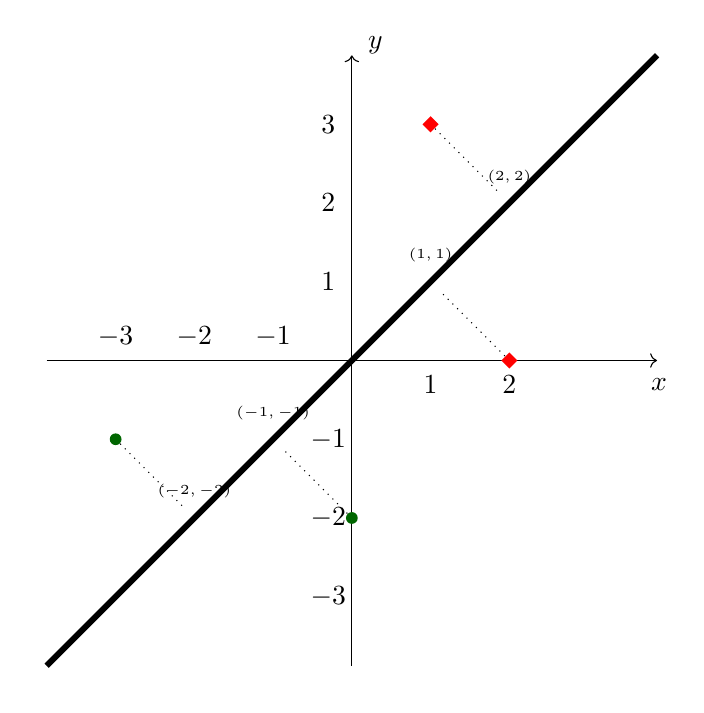
\begin{tikzpicture}
					\node (origin) at (0, 0) {};
					\node (top) at ($(origin) + (0, 4)$) {};
					\node (bottom) at ($(origin) + (0, -4)$) {};
					\node (left) at ($(origin) + (-4, 0)$) {};
					\node (right) at ($(origin) + (4, 0)$) {};
					\draw [->] (bottom) -- (top);
					\draw [->] (left) -- (right);
			
					\node at (-4, -4) (leftendpoint) {};
					\node at (4, 4) (rightendpoint) {};
					%\node at ($(origin) + (0.8, 1.3)$) {$y=\alpha x$};
					\node at ($(origin) + (3.9, -0.3)$) {$x$};
					\node at ($(origin) + (0.3, 4.0)$) {$y$};
			
					\draw[line width=0.75mm] (leftendpoint) -- (rightendpoint);
			
					\node[circle, fill=black!60!green, inner sep=1.5pt] at ($({-3/1.0}, {-1/1.0})$) (dp1) {};
					\node[circle, fill=black!60!green, inner sep=1.5pt] at ($({0/1.0}, {-2/1.0})$) (dp2) {};
					\node[diamond, fill=red, inner sep=1.5pt] at ($({2/1.0}, {0/1.0})$) (dp3) {};
					\node[diamond, fill=red, inner sep=1.5pt] at ($({1/1.0}, {3/1.0})$) (dp4) {};
					

					\node[label= {\tiny $\left( -2, -2\right)$}] at (-2, -2) (r1) {};
					\node[label= {\tiny $\left( -1, -1\right)$}] at (-1, -1) (r2) {};
					\node[label= {\tiny $\left( 1, 1\right)$}] at (1, 1) (r3) {};
					\node[label= {\tiny $\left( 2, 2\right)$}] at (2, 2) (r4) {};

					\draw[dotted] (dp1) -- (r1);
					\draw[dotted] (dp2) -- (r2);
					\draw[dotted] (dp3) -- (r3);
					\draw[dotted] (dp4) -- (r4);
			
					\node at ($({1/1.0}, 0.1)$) (dp1x) {};
					\node at ($(-0.1, {-2/1.0})$) (dp1y) {};
					\node at ($({1/1.0}, -0.3)$) {$1$};
					\node at ($(-0.3, {-2/1.0})$) {$-2$};
					%\draw[dotted] (dp1) -- (dp1x);
					%\draw[dotted] (dp1) -- (dp1y);
			
					\node at ($({2/1.0}, -0.1)$) (dp2x) {};
					\node at ($(-0.1, {3/1.0})$) (dp2y) {};
					\node at ($({2/1.0}, -0.3)$) {$2$};
					\node at ($(-0.3, {1/1.0})$) {$1$};
					\node at ($(-0.3, {2/1.0})$) {$2$};
					\node at ($(-0.3, {3/1.0})$) {$3$};
					%\draw[dotted] (dp2) -- (dp2x);
					%\draw[dotted] (dp2) -- (dp2y);
			
					\node at ($({-3/1.0}, 0.1)$) (dp3x) {};
					\node at ($(0.1, {-1/1.0})$) (dp3y) {};
					\node at ($({-3/1.0}, 0.3)$) {$-3$};
					\node at ($({-2/1.0}, 0.3)$) {$-2$};
					\node at ($({-1/1.0}, 0.3)$) {$-1$};
					\node at ($(-0.3, {-3/1.0} )$) {$-3$};
					\node at ($(-0.3, {-1/1.0} )$) {$-1$};
					%\draw[dotted] (dp3) -- (dp3x);
					%\draw[dotted] (dp3) -- (dp3y);
			
			
					\node[inner sep=0pt] at ($(leftendpoint)!(dp1)!(rightendpoint)$) (pdp1) {};
					\node[inner sep=0pt] at ($(leftendpoint)!(dp2)!(rightendpoint)$) (pdp2) {};
					\node[inner sep=0pt] at ($(leftendpoint)!(dp3)!(rightendpoint)$) (pdp3) {};
			
					%\draw[red] (dp1) -- (pdp1);
					%\draw[red] (dp2) -- (pdp2);
					%\draw[red] (dp3) -- (pdp3);
				\end{tikzpicture}
\end{Described}
				\caption{Plot of Transactions in 2-D}
			\end{figure}
		}


\end{enumerate}

  \newpage
  \qns{Diode System ID (Adapted from EECS 16B Fall 2023 Final)}

    \textbf{Note: This problem does not require knowledge of circuits or diodes.}
    
    Suppose that we want to characterize a diode $D_1$ with parasitic resistance $R_p$, represented by the following model:
    \begin{figure}[H]
        \begin{center}
            \begin{Described}{Voltage source V sub B drives from ground up to the top node, where diode D1 carries current I D to the right with voltage V D across it, in series with resistor R sub p returning to ground.}
\begin{circuitikz}
                \draw (0, 2) to [V, l_=$V_B$] (0, 0) node[ground]{}
                (0, 2) to [Do, l=$D_1$, i=$I_D$, v=$V_D$] (3, 2) to [R, l=$R_p$] (5, 2) node[ground]{}
                ;
            \end{circuitikz}
\end{Described}
        \end{center}
    \end{figure}
    The current through the diode (forward-biased) is modeled as
    \begin{equation}
        I_D = I_0\e^{\frac{V_D}{V_T}}
    \end{equation}
    where $V_D$ is the voltage across the diode (as shown in the diagram), $I_0$ is a parameter associated with the diode, and $V_T$ is the thermal voltage, a temperature dependent variable.
    
    With some analysis, the system equation can be simplified to:
    \begin{equation}
        I_D = I_0 \e^{\frac{V_B - I_D R_p}{V_T}}
    \end{equation}
    To collect data, we will vary the temperature to vary $V_T$ and measure the current $I_D$ through the diode.
    
        \begin{enumerate}

            \qitem    Use the provided system equation to show that
                \begin{equation}
                    I_D R_p - V_T \ln(I_0) = V_B - V_T \ln(I_D)
                \end{equation}
                    is a valid equation to represent the system.
                \begin{hint}
                    Use the logarithm identity $\ln(\frac{a}{b}) = \ln(a) - \ln(b)$.
                \end{hint}
            
    
            \ans{
                \begin{align}
                    I_D &= I_0 \e^{\frac{V_B - I_D R_p}{V_T}} \\
                    V_T\ln(\frac{I_D}{I_0}) &= V_B - I_D R_p \\
                    V_T\ln(I_D) - V_T\ln(I_0) &= V_B - I_D R_p \\
                    I_D R_p - V_T \ln(I_0) &= V_B - V_T \ln(I_D)
                \end{align}
            }
    
            % \begin{problempart}{4}{System ID}{0}{0}
            %     Suppose we use $V_B = 1 \mathrm{V}$ and collect the following data points:
            %     \begin{itemize}
            %         \item For $V_T = 0.025 \mathrm{V}$, $I_D = 0.0185 \mathrm{A}$.
            %         \item For $V_T = 0.05 \mathrm{V}$, $I_D = 0.0172 \mathrm{A}$.
            %         \item For $V_T = 0.0125 \mathrm{V}$, $I_D = 0.0193 \mathrm{A}$.
            %     \end{itemize}
            %     \textbf{Find the matrix $D$ and vector $\vec{s}$ to set up a least-squares problem $D\vec{p} \approx \vec{s}$ where $\vec{p} = \begin{bmatrix} \ln(I_0) \\ R_p \end{bmatrix}$.}
    
            %     You do not have to simplify the elements $D$ and $\vec{s}$, but the elements should be numerical values, not in terms of variables.
            % \end{problempart}
    
            % \begin{solution}{4in}
            %     Each data point can be used with the provided system equation from the first part to create a system of linear equations with the unknowns being $\ln(I_0)$ and $R_p$ (remember that the problem provides that $V_B = 1 \mathrm{V}$):
            %     \begin{itemize}
            %         \item $-0.025\ln(I_0) + 0.0185R_p = 1 - 0.025\ln(0.0185)$
            %         \item $-0.05\ln(I_0) + 0.0172R_p = 1 - 0.05\ln(0.0172)$
            %         \item $-0.0125\ln(I_0) + 0.0193R_p = 1 - 0.0125\ln(0.0193)$
            %     \end{itemize}
            %     The matrix form of this system is:
            %     \begin{equation}
            %         \begin{bmatrix} -0.025 & 0.0185 \\ -0.05 & 0.0172 \\ -0.0125 & 0.0193 \end{bmatrix} \begin{bmatrix} \ln(I_0) \\ R_p \end{bmatrix} = \begin{bmatrix} 1 - 0.025\ln(0.0185) \\ 1 - 0.05\ln(0.0172) \\ 1 - 0.0125\ln(0.0193) \end{bmatrix}
            %     \end{equation}
            %     Thus, for the least-squares problem, $D = \begin{bmatrix} -0.025 & 0.0185 \\ -0.05 & 0.0172 \\ -0.0125 & 0.0193 \end{bmatrix}$ and $\vec{s} = \begin{bmatrix} 1 - 0.025\ln(0.0185) \\ 1 - 0.05\ln(0.0172) \\ 1 - 0.0125\ln(0.0193) \end{bmatrix}$
            % \end{solution}
    
            \vspace{5cm}
            
            \qitem    Suppose we use $V_B = v_B$ and collect the following data points:
                \begin{itemize}
                    \item For $V_T = v_{T1}$, $I_D = i_{D1}$.
                    \item For $V_T = v_{T2}$, $I_D = i_{D2}$.
                    \item For $V_T = v_{T3}$, $I_D = i_{D3}$.
                \end{itemize}
                Find the matrix $\textbf{A}$ and vector $\vec{x}$ to set up a least-squares problem $\textbf{A} \vec{x} \approx \vec{b}$ where $\vec{x} = \begin{bmatrix} \ln(I_0) \\ R_p \end{bmatrix}$
    
            \ans{
                Each data point can be used with the provided system equation from the first part to create a system of linear equations with the unknowns being $\ln(I_0)$ and $R_p$ (remember that the problem provides that $V_B = v_B$):
                \begin{itemize}
                    \item $-v_{T1}\ln(I_0) + i_{D1}R_p = v_B - v_{T1}\ln(i_{D1})$
                    \item $-v_{T2}\ln(I_0) + i_{D2}R_p = v_B - v_{T2}\ln(i_{D2})$
                    \item $-v_{T3}\ln(I_0) + i_{D3}R_p = v_B - v_{T3}\ln(i_{D3})$
                \end{itemize}
                The matrix form of this system is:
                \begin{equation}
                    \begin{bmatrix} -v_{T1} & i_{D1} \\ -v_{T2} & i_{D2} \\ -v_{T3} & i_{D3} \end{bmatrix} \begin{bmatrix} \ln(I_0) \\ R_p \end{bmatrix} = \begin{bmatrix} v_B - v_{T1}\ln(i_{D1}) \\ v_B - v_{T2}\ln(i_{D2}) \\ v_B - v_{T3}\ln(i_{D3}) \end{bmatrix}
                \end{equation}
                Thus, for the least-squares problem, $\textbf{A} = \begin{bmatrix} -v_{T1} & i_{D1} \\ -v_{T2} & i_{D2} \\ -v_{T3} & i_{D3} \end{bmatrix}$ and $\vec{b} = \begin{bmatrix} v_B - v_{T1}\ln(i_{D1}) \\ v_B - v_{T2}\ln(i_{D2}) \\ v_B - v_{T3}\ln(i_{D3}) \end{bmatrix}$
            }
            
            \vspace{5cm}
            
            \qitem    Explain how you would use the least-squares system from the previous part to find model parameters $I_0$ and $R_p$. You do not need to use actual values for this part; you explanation can just use $\textbf{A}$ and $\vec{b}$ as known variables to show what calculations you would do to find $I_0$ and $R_p$.
            
    
            \ans{
                We would first find the optimal parameter $\hat{\vec{x}}$ with the least squares formula:
                \begin{equation}
                    \hat{\vec{x}} = (\textbf{A}^\top \textbf{A})^{-1} \textbf{A}^{\top} \vec{b}
                \end{equation}
                The elements of $\hat{\vec{x}}$ represent optimal values for $\ln(I_0)$ and $R_p$ so we set the elements of $\hat{\vec{x}}$ equal to those parameters for our model:
                \begin{align}
                    \hat{x}_{v_B} = \ln(I_0) &\rightarrow I_0 = \e^{\hat{x}_1} \\
                    \hat{x}_2 = R_p &\rightarrow R_p = \hat{x}_2
                \end{align}
                Thus, we have found parameter values for $I_0$ and $R_p$ from the least-squares system.
            }
    
        \end{enumerate}

\end{qunlist}

\end{document}
"

\DocumentMetadata{
  lang       = en-US,
  pdfversion = 2.0,
  testphase  = {phase-III,math,table,graphic,firstaid},
}
\documentclass{latexally-assignment}

\usepackage{amsmath,amssymb}
\usepackage{float}
\usepackage{tikz}
\usetikzlibrary{calc,shapes.geometric,positioning}
\usepackage[american]{circuitikz}

% The corpus macros these four files use, reproduced from questionBank/ee16.sty
% and questionBank/sp26/sp26.sty so the demo does not need the whole course
% preamble chain. Same meanings, nothing more.
\providecommand{\bmqty}[1]{\begin{bmatrix}#1\end{bmatrix}}
\providecommand{\e}{\mathop{\mathrm{e}}\nolimits}
\providecommand{\wt}[1]{\widetilde{#1}}
\NewDocumentEnvironment{hint}{+b}{\itshape (HINT: #1)}{}

\setcoursenumber{EECS 16A}
\setcoursename{Designing Information Devices and Systems I}
\setsemester{Spring 2026}

\begin{document}

\def\title{Described figures from the question bank}
\maketitle

\vspace{0.5em}
Every figure below carries a description in the PDF structure tree. A screen
reader announces "graphic" and then that description; it never reaches the
drawing underneath. Hovering shows nothing --- \texttt{/Alt} is not a tooltip.

\begin{qunlist}

  \qns{Polynomial Multiplication and Discrete-Time Convolution [Adapted from EE 120]}
% Adapted and extended by Ken Zheng for EECS 16A Fall 2025 Discussion

The impulse response of a real, discrete-time FIR filter $\mathsf{A}$ is described by  
$$a[n]=a_0 \delta[n]+a_1 \delta[n-1]+\cdots + a_N \delta[n-N], \quad \text{where } N\in \{1,2,3,\ldots\}.$$

\begin{enumerate}[(a)]
\item Show that the frequency response $A(\omega)$ of the filter is a polynomial, in terms of $e^{-i\omega}$, whose coefficients have a simple relationship with the impulse response values $a_0,\ldots,a_N$.

\ans{

    Substituting \(a[n]\) into the frequency response formula we see that:
    \begin{equation*}
        A(w) = \sum_{n=-\infty}^{\infty} a[n]e^{-iwn}
    \end{equation*}
    As $a[n] = 0$ outside the range of $n = 0$ to $n = N$ ,
    \begin{equation*}
        A(w) = a_0 e^{-iw\cdot 0} + a_1 e^{-iw\cdot 1} + \ldots + a_N e^{-iw\cdot N}
    \end{equation*}
    \begin{equation*}
        = a_0 + a_1 e^{-iw} + \ldots + a_N e^{-iwN}
    \end{equation*}
}
\item Suppose the filter $\mathsf{A}$ is placed in a cascade (series) interconnection with another discrete-time FIR filter $\mathsf{B}$ whose impulse response is described by  
$$b[n]=b_0 \delta[n]+b_1 \delta[n-1]+\cdots + b_M \delta[n-M],\quad \text{where } M\in \{1,2,3,\ldots\}.$$

The cascade structure, which we call $\mathsf{C}$, is shown in the figure below.
\vspace{4pt}

\centerline{
    \begin{Described}{Block diagram: input x enters block A, whose output feeds block B, and block B's output is y. An outer box enclosing both blocks is labelled C.}
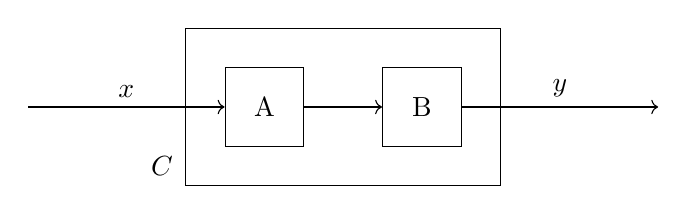
\begin{tikzpicture}
        % Define nodes for blocks A and B
        \node[draw, rectangle, minimum width=1cm, minimum height=1cm] (A) at (0,0) {A};
        \node[draw, rectangle, minimum width=1cm, minimum height=1cm] (B) at (2,0) {B};
        
        % Draw the outer rectangle
        \draw (-1, 1) rectangle (3, -1);
        
        % Draw arrows and labels
        \draw[->] (-3, 0) -- (A.west) node[midway,above] {$x$};
        \draw[->] (A.east) -- (B.west);
        \draw[->] (B.east) -- (5, 0) node[midway,above] {$y$};
        
        % Label C 
        \node at (-1.3, -0.5) [below] {$C$};
    \end{tikzpicture}
\end{Described}
}
Let $c$ denote the impulse response of the cascade interconnection.

\begin{enumerate}[(i)]
\item Express $c$ in terms of $a$ and $b$.
    
\ans{

        The impulse response \(c\) of the cascade interconnection is given by 
        \begin{equation*}
            c[n] = (a * b)[n] = \sum_{k=-\infty}^{\infty} a[k]\,b[n-k]
        \end{equation*}
         Substituting \(n = 0\):
        \begin{equation*}
            c_0 = a_0 b_0
        \end{equation*}
        \(n = 1\):
        \begin{equation*}
            c_1 = a_0 b_1 + a_1 b_0 
        \end{equation*}
        \(n = 2\):
        \begin{equation*}
            c_2 = a_0 b_2 + a_1 b_1 + a_2 b_0
        \end{equation*}
        And so on...
    
        Thus, we can write:
        \begin{equation*}
            c_n = \sum_{k=\max(0,n-M)}^{\min(n, N)} a_k b_{n-k}
        \end{equation*}
        \null\hfill for \(n = 0, 1, \ldots, N + M\)
        
        where we found the bounds of summation from the two conditions that ensure we are indexing \(a[n]\) and \(b[n]\) without exceeding the bounds of their signal.
        $$ 0 \leq k \leq N \Longrightarrow k \leq N \quad \text{and} \quad k \geq 0 $$
        $$ 0 \leq n - k \leq M \Longrightarrow k \leq n \quad \text{and} \quad k \geq n - M $$
        and so
        $$ k \leq \min(n, N) \quad \text{and} \quad k \geq \max(0, n-M) $$

        Lastly, 
         \begin{equation*}
            c[n] = c_0\delta[n] + c_1 \delta[n - 1] + ... + c_{N + M} \delta[n - ( N + M)]
        \end{equation*}
        
    }

\item Consider two polynomials $A(z)$ and $B(z)$ described as follows:
    $$
    A(z) = a_0 +a_1 z + \cdots + a_N z^N \quad \quad \quad B(z) = b_0 +b_1 z + \cdots + b_M z^M \, ,
    $$
    where $M$ and $N$ and positive integers.
    Let $C(z)=A(z)\, B(z)$, where $$ C(z) = c_0 +c_1 z + \cdots + c_{N+M} z^{N+M}.$$  Show that multiplying polynomials is tantamount to convolving their coefficients; in particular, explain how $c_n=(a*b)_n=\displaystyle\sum_m a_m b_{n-m}$, where $n={0,1,\ldots, N+M}$.
    
    \ans{
    \begin{equation*}
        C(z) = (a_0 +a_1 z + \cdots + a_N z^N) (b_0 +b_1 z + \cdots + b_M z^M)
    \end{equation*}
    \begin{equation*}
        C(z) = a_0 b_0 + (a_0 b_1 + a_1 b_0) z + (a_0 b_2 + a_1 b_1 + a_2 b_0) z^2 + ...
    \end{equation*}
    As you can see, each coefficient of \(z^n\) is the sum of all products of \(a_i\) and \(b_j\) where \(i + j = n\):
    \begin{equation*}
        c_n =  \sum_{m=\max(0,n-M)}^{\min(n, N)} a_m b_{n-m}
    \end{equation*}
    \null\hfill for \(n = 0, 1, 2, ..., N + M\)

    Just like the definition of convolution!
    }

\end{enumerate}
\end{enumerate}
  \newpage
  \qns{Frequency Response from a DAG Block Diagram [Adapted from EE 120]}
% Adapted by Ken Zheng for EECS 16A Fall 2025 Discussion

    Consider a DT LTI system with input $x[n]$ and output $y[n]$ that is implemented by the following block diagram:
    \begin{figure}[h!]
      \centering
      \begin{Described}{Block diagram: input x of n enters a summing junction whose output is y of n. That output is tapped, passed through a delay block D and then a gain of minus 0.5, and fed back into the summing junction.}
\begin{circuitikz}
          \node (x) at (0, 0) {$x[n]$};
          \node[circle, draw] (sum) at (2, 0) {$+$};
          % FIXME: find a better way to draw the triangle
          % \node[triangleblock, shape border rotate=90, inner sep=-1mm] (gain) at (3, -1.5) {$-0.5$};
          % \node at (3, -1.5) {$-0.5$};
          \node[draw, inner sep=5pt] (delay) at (6, -1.5) {$D$};
          \node (y) at (9, 0) {$y[n]$};
          \draw[->] (x.east) -- (sum.west);
          \draw[->] (sum.east) -- (y.west);
          \draw[->] (7.5, 0) -- (7.5, -1.5) -- (delay.east);
          % \draw[-, thick] (delay.west) -- (gain.east);
          % \draw[->, thick] (gain.west) -- (2, -1.5) -- (sum.south);
          \draw[->] (delay.west) to [amp, t=$-0.5$, blocks/scale=1.5] (2, -1.5) to (sum.south);
      \end{circuitikz}
\end{Described}
  \end{figure}
\begin{enumerate}
        \item Find the LCCDE that describes this system. 
        
        \ans{
            The difference equation describing this system is
              \begin{equation*}
                y[n] = x[n] - 0.5y[n-1]
              \end{equation*}
        }

        \item Find the frequency response $H(\omega)$ of this system. 
            
        \ans{
            Using the eigenfunction property by setting $x[n] = e^{i\omega n}$ and $y[n] = H(\omega) e^{i\omega n}$,
            \begin{align*}
            H(\omega) e^{i\omega n} &= e^{i\omega n} - 0.5 H(\omega) e^{i\omega (n-1)} \\
            &= e^{i\omega n} - 0.5 H(\omega) e^{-i\omega}e^{i\omega n} \\
            \left(1 + 0.5 e^{-i\omega}\right) e^{i\omega n} H(\omega) &= e^{i\omega n} \\
            H(\omega) &= \frac{e^{i\omega n}}{\left(1 + 0.5 e^{-i\omega}\right)e^{i\omega n}} \\
                &= \frac{1}{1 + 0.5 e^{-i\omega}}
            \end{align*} 
        } 

        \vspace{4cm}

        \item Is this a high pass or low pass filter?
        
        \ans{
            We can think about this in two ways:
            
            \textbf{1. Geometric Approach:}

            Recall from part (b) that the frequency response can be written as:
            \[
            H(\omega) = \frac{1}{1 + 0.5 e^{-i\omega}} = \frac{e^{i\omega}}{e^{i\omega} - (-0.5)}
            \]
            The magnitude is therefore:
            \[
            |H(\omega)| = \frac{1}{|e^{i\omega} - (-0.5)|}
            \]
            This represents the reciprocal of the distance from the point $e^{i\omega}$ on the unit circle to the point located at $-0.5$ on the real axis:

            \begin{center}
            \begin{Described}{Complex plane with real and imaginary axes and the unit circle centred at the origin. A point is marked at minus 0.5 on the real axis, with an arrow from it to the point e to the i omega on the circle.}
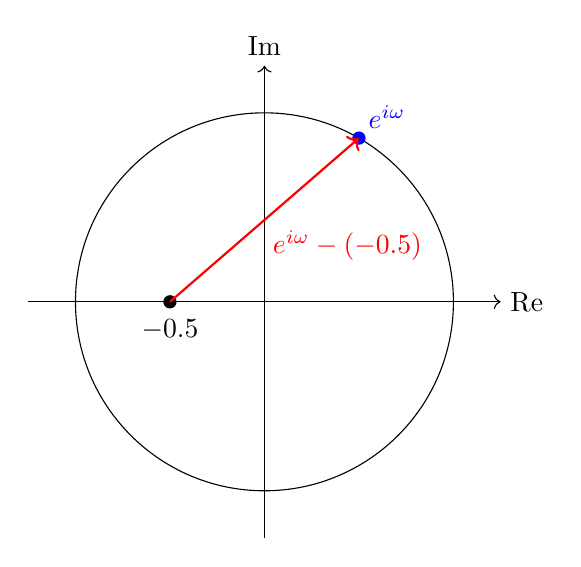
\begin{tikzpicture}[scale=1.2]
                % Axes
                \draw[->] (-2.5,0) -- (2.5,0) node[right] {$\operatorname{Re}$};
                \draw[->] (0,-2.5) -- (0,2.5) node[above] {$\operatorname{Im}$};

                % Unit circle
                \draw (0,0) circle (2);

                % Pole at -0.5
                \fill[black] (-1,0) circle (2pt) node[below left] {};
                \node[black] at (-1,-0.3) {$-0.5$};

                % Point on unit circle at angle ω
                \coordinate (P) at (60:2);
                \fill[blue] (P) circle (2pt) node[above right] {$e^{i\omega}$};

                % Vector from pole to point on circle
                % \draw[->, thick, red] (-1,0) -- (P);
                \draw[->, thick, red] (-1,0) -- (P) node[midway, below] {$\qquad\qquad\qquad e^{i \omega} - (-0.5)$};  % Label added here


                % Labels
                \node at (1.8,1.8) {};
            \end{tikzpicture}
\end{Described}
            \end{center}

            Key observations:
            \begin{itemize}
                \item When $\omega = 0$, $e^{i\omega} = 1$. The distance from $1$ to $-0.5$ is $1.5$, so $|H(0)| = 1/1.5 \approx 0.667$.
                \item When $\omega = \pi$, $e^{i\omega} = -1$. The distance from $-1$ to $-0.5$ is $0.5$, so $|H(\pi)| = 1/0.5 = 2$.
                \item As $\omega$ moves from $0$ to $\pi$, the point $e^{i\omega}$ travels along the upper half of the unit circle from $(1,0)$ to $(-1,0)$. 
                The distance to the point at $-0.5$ decreases monotonically, so $|H(\omega)|$ increases. Thus, we have a high-pass filter!\\
            \end{itemize}

            
            \textbf{2. Algebraic Approach:}
            
            To determine the filter type, we simplify the magnitude of the frequency response first:

            \[
            |H(\omega)| = \frac{1}{\sqrt{(1 + 0.5\cos\omega)^2 + (0.5\sin\omega)^2}}
            \]


            Expanding \( (1 + 0.5\cos\omega)^2 \) and \( (0.5\sin\omega)^2 \):
            \[
            (1 + 0.5\cos\omega)^2 = 1^2 + 2(1)(0.5\cos\omega) + (0.5\cos\omega)^2 = 1 + \cos\omega + 0.25\cos^2\omega
            \]
            \[
            (0.5\sin\omega)^2 = 0.25\sin^2\omega
            \]


            Add the two results in the square root:
            \[
            (1 + 0.5\cos\omega)^2 + (0.5\sin\omega)^2 = \left[1 + \cos\omega + 0.25\cos^2\omega\right] + \left[0.25\sin^2\omega\right]
            \]
            \[
            = 1 + \cos\omega + 0.25\left(\cos^2\omega + \sin^2\omega\right)
            \]
            \[
            = 1 + \cos\omega + 0.25(1) = 1 + \cos\omega + 0.25 = 1.25 + \cos\omega
            \]


            Substitute back into \( |H(\omega)| \):
            \[
            |H(\omega)| = \frac{1}{\sqrt{1.25 + \cos\omega}}
            \]
                        
            Now we analyze the magnitude at key frequencies:
            
            Low frequency (\( \omega = 0 \)): 
                \[
                |H(0)| =  \frac{1}{\sqrt{1.25 + \cos0}} = \frac{1}{1.5} \approx 0.667 \quad (\text{attenuated})
                \]
            High frequency (\( \omega = \pi \)): 
                \[
                |H(\pi)| =  \frac{1}{\sqrt{1.25 + \cos\pi}} = 2 \quad (\text{passed})
                \]

            We can see that, again, the filter attenuates low frequencies and passes high frequencies, so it is a high-pass filter!\\

            Both geometrically and algebraically, we conclude this is a \textbf{high-pass filter}. Nice!
        }
\end{enumerate}

  \newpage
  \qns{Using PCA to Detect Fraudulent Transactions (Adapted from EECS 16B Spring 2023 Final)}\\
	PCA has many different uses when applied to real-world data. One potential application is making classification of data much easier.
	
	Suppose we are given some data, where each datapoint represents a transaction. Each one is labeled either normal or fraudulent. We will utilize PCA to develop a useful classifier.

	We plot the data in two dimensions, where each dimension is some unspecified feature that will aid us in classifying the points:

	\begin{figure}[H]
        \centering
        \begin{Described}{Scatter plot on x and y axes running about minus 4 to 4, with four transactions marked: circles at (-3, -1) and (0, -2), and diamonds at (2, 0) and (1, 3).}
\begin{tikzpicture}
            \node (origin) at (0, 0) {};
            \node (top) at ($(origin) + (0, 4)$) {};
            \node (bottom) at ($(origin) + (0, -4)$) {};
            \node (left) at ($(origin) + (-4, 0)$) {};
            \node (right) at ($(origin) + (4, 0)$) {};
            \draw [->] (bottom) -- (top);
            \draw [->] (left) -- (right);
    
            \node at (-3, -2.2) (leftendpoint) {};
            \node at (3, 2.2) (rightendpoint) {};
            %\node at ($(origin) + (0.8, 1.3)$) {$y=\alpha x$};
            \node at ($(origin) + (3.9, -0.3)$) {$x$};
            \node at ($(origin) + (0.3, 4.0)$) {$y$};
    
            %\draw[line width=0.75mm] (leftendpoint) -- (rightendpoint);
    
            \node[circle, fill=black!60!green, inner sep=1.5pt] at ($({-3/1.0}, {-1/1.0})$) (dp1) {};
            \node[circle, fill=black!60!green, inner sep=1.5pt] at ($({0/1.0}, {-2/1.0})$) (dp2) {};
            \node[diamond, fill=red, inner sep=1.5pt] at ($({1/1.0}, {3/1.0})$) (dp3) {};
			\node[diamond, fill=red, inner sep=1.5pt] at ($({2/1.0}, {0/1.0})$) (dp4) {};
    
            \node at ($({1/1.0}, 0.1)$) (dp1x) {};
            \node at ($(-0.1, {-2/1.0})$) (dp1y) {};
            \node at ($({1/1.0}, 0.3)$) {$1$};
            \node at ($(-0.3, {-2/1.0})$) {$-2$};
            %\draw[dotted] (dp1) -- (dp1x);
            %\draw[dotted] (dp1) -- (dp1y);
    
            \node at ($({2/1.0}, -0.1)$) (dp2x) {};
            \node at ($(-0.1, {3/1.0})$) (dp2y) {};
            \node at ($({2/1.0}, -0.3)$) {$2$};
            \node at ($(-0.3, {3/1.0})$) {$3$};
            %\draw[dotted] (dp2) -- (dp2x);
            %\draw[dotted] (dp2) -- (dp2y);
    
            \node at ($({-3/1.0}, 0.1)$) (dp3x) {};
            \node at ($(0.1, {-1/1.0})$) (dp3y) {};
            \node at ($({-3/1.0}, 0.3)$) {$-3$};
            \node at ($(-0.3, {-1/1.0 -0.3} )$) {$-1$};
            %\draw[dotted] (dp3) -- (dp3x);
            %\draw[dotted] (dp3) -- (dp3y);
    
    
            \node[inner sep=0pt] at ($(leftendpoint)!(dp1)!(rightendpoint)$) (pdp1) {};
            \node[inner sep=0pt] at ($(leftendpoint)!(dp2)!(rightendpoint)$) (pdp2) {};
            \node[inner sep=0pt] at ($(leftendpoint)!(dp3)!(rightendpoint)$) (pdp3) {};
    
            %\draw[red] (dp1) -- (pdp1);
            %\draw[red] (dp2) -- (pdp2);
            %\draw[red] (dp3) -- (pdp3);
        \end{tikzpicture}
\end{Described}
        \caption{Plot of Transactions in 2-D}
	\end{figure}

	Thus, we have a total of 4 transactions, $\bmqty{-3 \\ -1}$ and $\bmqty{0 \\ -2}$ are normal, while $\bmqty{2 \\ 0}$ and $\bmqty{1 \\ 3}$ are fraudulent.
	\begin{enumerate}
		%Part A:
		
		\qitem Suppose we now construct a data matrix, where the \textit{data points are columns}. 

			\begin{equation}
				X = \bmqty{-3 & 0 & 2 & 1 \\ -1 & -2 & 0 & 3}
			\end{equation}

			Using this data matrix, \textbf{calculate its first principal component $\vec{u}_1$}.

			\begin{hint}
			\begin{enumerate}

				\item You may also make use of the fact that $XX^T$ is given by:
				\begin{align}
					XX^{\top} &= \bmqty{-3 & 0 & 2 & 1 \\ -1 & -2 & 0 & 3}\bmqty{-3 & 0 & 2 & 1 \\ -1 & -2 & 0 & 3}^{\top} \\
						&= \bmqty{14 & 6 \\ 6 & 14}
				\end{align}
				\item You may also make use of the characteristic polynomial of $XX^T$:
				\begin{equation}
					\lambda^2 - 28\lambda + 160 = (\lambda - 20)(\lambda - 8) = 0
				\end{equation}
			\end{enumerate}
			\end{hint}
			
			\begin{hint} Remember that your principal component should be of unit norm. \end{hint}

		\ans{
			% From PCA, we know that our first principal component of a matrix with column data is the first column vector of $U$ in the SVD of $X$. Thus, we use the SVD method of calculation (find the eigenvector corresponding to the largest eigenvalue of $XX^{\top}$ and normalize to yield $\vec{u}_1$).

			% \begin{align}
			% 	XX^{\top} &= \bmqty{-3 & 0 & 2 & 1 \\ -1 & -2 & 0 & 3}\bmqty{-3 & 0 & 2 & 1 \\ -1 & -2 & 0 & 3}^{\top} \\
			% 		 &= \bmqty{14 & 6 \\ 6 & 14}
			% \end{align}

			% From setting $\mathrm{det}(XX^{\top} - \lambda I) = 0$, we should find our characteristic polynomial to be 
			
			% \begin{equation}
			% 	\lambda^2 - 28\lambda + 160 = 0
			% \end{equation}

			Our eigenvalues are $\lambda_1 = 20$ and $\lambda_2 = 8$. Thus, the eigenvector corresponding to our largest eigenvalue $\lambda_1 = 20$ is $\vec{v}_1 = \bmqty{1 \\ 1}$ from inspection.
			
			Thus, our principal component vector is given as the normalized eigenvector: i.e. $\vec{u}_1 = \bmqty{\frac{1}{\sqrt{2}} \\ \frac{1}{\sqrt{2}}}$.
        }

		%Part B:
		
		\qitem	It's difficult to come up with a useful classifier in two dimensions. Let's use PCA dimensionality reduction to help.
			
			Using your answer in part (a), \textbf{project your two-dimensional data points onto one dimension. Express your answer as the vector $\vec{z} \in \mathbb{R}^{1 \times 4}$.}

		\ans{
			To project our 2-d data into 1-d, we project our data matrix onto the first principal component as follows:
			
			\begin{equation}
				\vec{z} = \vec{u}_1^{\top}X = \bmqty{\frac{1}{\sqrt{2}} \\ \frac{1}{\sqrt{2}}} \bmqty{-3 & 0 & 2 & 1 \\ -1 & -2 & 0 & 3} = \bmqty{-\frac{4}{\sqrt{2}} & -\frac{2}{\sqrt{2}} & \frac{2}{\sqrt{2}} & \frac{4}{\sqrt{2}}}
			\end{equation}
		}
		
		%Part C:
		
		\qitem	Now, plot each of these points, on the line below. Indicate the value and label (normal as circle and fraudulent as diamond) for each point.
			
			\textit{Note: your plot doesn't have to be to scale.}

			\begin{figure}[H]
				\centering
				\begin{Described}{Blank horizontal number line labelled z, with only the origin marked 0 and no points plotted.}
\begin{tikzpicture}
					\node (origin) at (0, 0) {|};
            		%\node (top) at ($(origin) + (0, 4)$) {};
            		%\node (bottom) at ($(origin) + (0, -4)$) {};
            		\node (left) at ($(origin) + (-4, 0)$) {};
            		\node (right) at ($(origin) + (4, 0)$) {};
					\node at ($(origin) + (3.9, -0.3)$) {$z$};
					\node at ($(origin) + (0, -0.3)$) {0};
            		%\draw [->] (bottom) -- (top);
            		\draw [<->] (left) -- (right);

				\end{tikzpicture}
\end{Described}
				\caption{Plot of Transactions in 1-D}
			\end{figure}

		\ans{
			\begin{figure}[H]
				\centering
				\begin{Described}{Number line labelled z with the origin marked 0 and four points: circles at minus four over root two and minus two over root two, diamonds at two over root two and four over root two.}
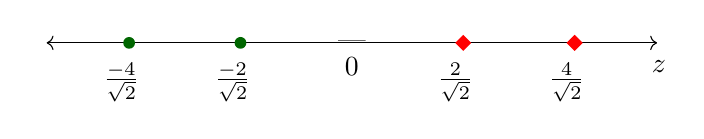
\begin{tikzpicture}
					\node (origin) at (0, 0) {|};
            		%\node (top) at ($(origin) + (0, 4)$) {};
            		%\node (bottom) at ($(origin) + (0, -4)$) {};
            		\node (left) at ($(origin) + (-4, 0)$) {};
            		\node (right) at ($(origin) + (4, 0)$) {};
					\node at ($(origin) + (3.9, -0.3)$) {$z$};
					\node at ($(origin) + (0, -0.3)$) {0};
            		%\draw [->] (bottom) -- (top);
            		\draw [<->] (left) -- (right);

					\node[circle, fill=black!60!green, inner sep=1.5pt] at ($(origin) + (-4/1.414, 0)$) (dp1) {};
					\node at ($(origin) + (-4/1.414 -0.1, -0.5)$) {$\frac{-4}{\sqrt{2}}$};
					\node[circle, fill=black!60!green, inner sep=1.5pt] at ($(origin) + (-2/1.414, 0)$) (dp1) {};
					\node at ($(origin) + (-2/1.414 -0.1, -0.5)$) {$\frac{-2}{\sqrt{2}}$};
					\node[diamond, fill=red, inner sep=1.5pt] at ($(origin) + (2/1.414, 0)$) (dp1) {};
					\node at ($(origin) + (2/1.414 -0.1, -0.5)$) {$\frac{2}{\sqrt{2}}$};
					\node[diamond, fill=red, inner sep=1.5pt] at ($(origin) + (4/1.414, 0)$) (dp1) {};
					\node at ($(origin) + (4/1.414 -0.1, -0.5)$) {$\frac{4}{\sqrt{2}}$};
				\end{tikzpicture}
\end{Described}
				\caption{Plot of Transactions in 1-D}
			\end{figure}
		}

		%Part D:
		
		\qitem	Suppose you are given some transaction datapoint, $\vec{x}_i$ and you project it to be one-dimensional, i.e. $z_i$. \textbf{Based on your plot from part (c), come up with an inequality in terms of $z_i$ to identify if that transaction is fraudulent.}
			
			\textit{Note: There can be more than one answer, but please only give one.}

		\ans{
			$\vec{z}_i > 0$ is a possible answer. In fact any answer in between $\vec{z}_i \geq -\frac{2}{\sqrt{2}}$ and $\vec{z}_i \geq \frac{2}{\sqrt{2}}$ is valid.
		}

		%Part E:
		
		\qitem	It can often be informative to compare our original data with its PCA reconstructions. \textbf{Using PCA, reconstruct $\vec{z}$ back into 2-D as the matrix $\wt{X} \in \mathbb{R}^{2 \times 4}$.}

		\ans{
			Using the reconstruction principle of PCA, we lift the 1D data back into 2 dimensions by doing the following:
			\begin{equation}
				\wt{X} = \vec{u}_1\vec{u}_1^{\top}X = \bmqty{-2 & -1 & 1 & 2 \\ -2 & -1 & 1 & 2}
			\end{equation}
		}

		%Part F:
		
		\qitem	Finally, we visualize our PCA reconstruction. \textbf{On the graph below, draw your first principal component direction (extend it as a solid line in both directions). Draw your reconstructioned points from $\wt{X}$, with dotted lines connecting them with the corresponding point in $X$. } You may draw on the plot on the next page.

			\begin{figure}[H]
				\centering
				\begin{Described}{Scatter plot on x and y axes running about minus 4 to 4, with four transactions marked: circles at (-3, -1) and (0, -2), and diamonds at (2, 0) and (1, 3).}
\begin{tikzpicture}
					\node (origin) at (0, 0) {};
					\node (top) at ($(origin) + (0, 4)$) {};
					\node (bottom) at ($(origin) + (0, -4)$) {};
					\node (left) at ($(origin) + (-4, 0)$) {};
					\node (right) at ($(origin) + (4, 0)$) {};
					\draw [->] (bottom) -- (top);
					\draw [->] (left) -- (right);
			
					\node at (-3, -2.2) (leftendpoint) {};
					\node at (3, 2.2) (rightendpoint) {};
					%\node at ($(origin) + (0.8, 1.3)$) {$y=\alpha x$};
					\node at ($(origin) + (3.9, -0.3)$) {$x$};
					\node at ($(origin) + (0.3, 4.0)$) {$y$};
			
					%\draw[line width=0.75mm] (leftendpoint) -- (rightendpoint);
			
					\node[circle, fill=black!60!green, inner sep=1.5pt] at ($({-3/1.0}, {-1/1.0})$) (dp1) {};
					\node[circle, fill=black!60!green, inner sep=1.5pt] at ($({0/1.0}, {-2/1.0})$) (dp2) {};
					\node[diamond, fill=red, inner sep=1.5pt] at ($({1/1.0}, {3/1.0})$) (dp3) {};
					\node[diamond, fill=red, inner sep=1.5pt] at ($({2/1.0}, {0/1.0})$) (dp4) {};
			
					\node at ($({1/1.0}, 0.1)$) (dp1x) {};
					\node at ($(-0.1, {-2/1.0})$) (dp1y) {};
					\node at ($({1/1.0}, 0.3)$) {$1$};
					\node at ($(-0.3, {-2/1.0})$) {$-2$};
					%\draw[dotted] (dp1) -- (dp1x);
					%\draw[dotted] (dp1) -- (dp1y);
			
					\node at ($({2/1.0}, -0.1)$) (dp2x) {};
					\node at ($(-0.1, {3/1.0})$) (dp2y) {};
					\node at ($({2/1.0}, -0.3)$) {$2$};
					\node at ($(-0.3, {3/1.0})$) {$3$};
					%\draw[dotted] (dp2) -- (dp2x);
					%\draw[dotted] (dp2) -- (dp2y);
			
					\node at ($({-3/1.0}, 0.1)$) (dp3x) {};
					\node at ($(0.1, {-1/1.0})$) (dp3y) {};
					\node at ($({-3/1.0}, 0.3)$) {$-3$};
					\node at ($(-0.3, {-1/1.0 -0.3} )$) {$-1$};
					%\draw[dotted] (dp3) -- (dp3x);
					%\draw[dotted] (dp3) -- (dp3y);
			
			
					\node[inner sep=0pt] at ($(leftendpoint)!(dp1)!(rightendpoint)$) (pdp1) {};
					\node[inner sep=0pt] at ($(leftendpoint)!(dp2)!(rightendpoint)$) (pdp2) {};
					\node[inner sep=0pt] at ($(leftendpoint)!(dp3)!(rightendpoint)$) (pdp3) {};
			
					%\draw[red] (dp1) -- (pdp1);
					%\draw[red] (dp2) -- (pdp2);
					%\draw[red] (dp3) -- (pdp3);
				\end{tikzpicture}
\end{Described}
				\caption{Plot of Transactions in 2-D}
			\end{figure}

		\ans{

			Using the answer from part (d), students should end up with the following graph:
			\begin{figure}[H]
				\centering
				\begin{Described}{The same four transactions, with a solid line through the origin along y = x and reconstructed points on it at (-2, -2), (-1, -1), (1, 1) and (2, 2), each joined to its original point by a dotted line.}
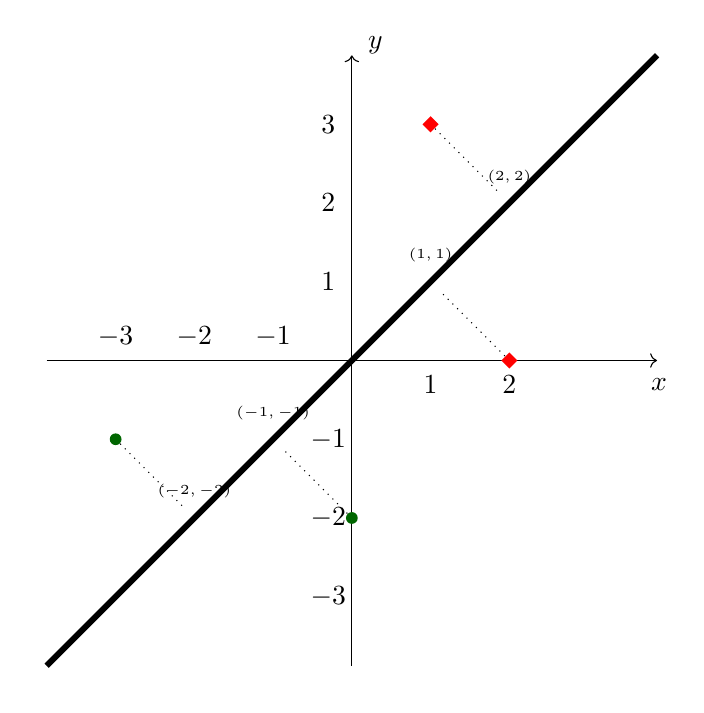
\begin{tikzpicture}
					\node (origin) at (0, 0) {};
					\node (top) at ($(origin) + (0, 4)$) {};
					\node (bottom) at ($(origin) + (0, -4)$) {};
					\node (left) at ($(origin) + (-4, 0)$) {};
					\node (right) at ($(origin) + (4, 0)$) {};
					\draw [->] (bottom) -- (top);
					\draw [->] (left) -- (right);
			
					\node at (-4, -4) (leftendpoint) {};
					\node at (4, 4) (rightendpoint) {};
					%\node at ($(origin) + (0.8, 1.3)$) {$y=\alpha x$};
					\node at ($(origin) + (3.9, -0.3)$) {$x$};
					\node at ($(origin) + (0.3, 4.0)$) {$y$};
			
					\draw[line width=0.75mm] (leftendpoint) -- (rightendpoint);
			
					\node[circle, fill=black!60!green, inner sep=1.5pt] at ($({-3/1.0}, {-1/1.0})$) (dp1) {};
					\node[circle, fill=black!60!green, inner sep=1.5pt] at ($({0/1.0}, {-2/1.0})$) (dp2) {};
					\node[diamond, fill=red, inner sep=1.5pt] at ($({2/1.0}, {0/1.0})$) (dp3) {};
					\node[diamond, fill=red, inner sep=1.5pt] at ($({1/1.0}, {3/1.0})$) (dp4) {};
					

					\node[label= {\tiny $\left( -2, -2\right)$}] at (-2, -2) (r1) {};
					\node[label= {\tiny $\left( -1, -1\right)$}] at (-1, -1) (r2) {};
					\node[label= {\tiny $\left( 1, 1\right)$}] at (1, 1) (r3) {};
					\node[label= {\tiny $\left( 2, 2\right)$}] at (2, 2) (r4) {};

					\draw[dotted] (dp1) -- (r1);
					\draw[dotted] (dp2) -- (r2);
					\draw[dotted] (dp3) -- (r3);
					\draw[dotted] (dp4) -- (r4);
			
					\node at ($({1/1.0}, 0.1)$) (dp1x) {};
					\node at ($(-0.1, {-2/1.0})$) (dp1y) {};
					\node at ($({1/1.0}, -0.3)$) {$1$};
					\node at ($(-0.3, {-2/1.0})$) {$-2$};
					%\draw[dotted] (dp1) -- (dp1x);
					%\draw[dotted] (dp1) -- (dp1y);
			
					\node at ($({2/1.0}, -0.1)$) (dp2x) {};
					\node at ($(-0.1, {3/1.0})$) (dp2y) {};
					\node at ($({2/1.0}, -0.3)$) {$2$};
					\node at ($(-0.3, {1/1.0})$) {$1$};
					\node at ($(-0.3, {2/1.0})$) {$2$};
					\node at ($(-0.3, {3/1.0})$) {$3$};
					%\draw[dotted] (dp2) -- (dp2x);
					%\draw[dotted] (dp2) -- (dp2y);
			
					\node at ($({-3/1.0}, 0.1)$) (dp3x) {};
					\node at ($(0.1, {-1/1.0})$) (dp3y) {};
					\node at ($({-3/1.0}, 0.3)$) {$-3$};
					\node at ($({-2/1.0}, 0.3)$) {$-2$};
					\node at ($({-1/1.0}, 0.3)$) {$-1$};
					\node at ($(-0.3, {-3/1.0} )$) {$-3$};
					\node at ($(-0.3, {-1/1.0} )$) {$-1$};
					%\draw[dotted] (dp3) -- (dp3x);
					%\draw[dotted] (dp3) -- (dp3y);
			
			
					\node[inner sep=0pt] at ($(leftendpoint)!(dp1)!(rightendpoint)$) (pdp1) {};
					\node[inner sep=0pt] at ($(leftendpoint)!(dp2)!(rightendpoint)$) (pdp2) {};
					\node[inner sep=0pt] at ($(leftendpoint)!(dp3)!(rightendpoint)$) (pdp3) {};
			
					%\draw[red] (dp1) -- (pdp1);
					%\draw[red] (dp2) -- (pdp2);
					%\draw[red] (dp3) -- (pdp3);
				\end{tikzpicture}
\end{Described}
				\caption{Plot of Transactions in 2-D}
			\end{figure}
		}


\end{enumerate}

  \newpage
  \qns{Diode System ID (Adapted from EECS 16B Fall 2023 Final)}

    \textbf{Note: This problem does not require knowledge of circuits or diodes.}
    
    Suppose that we want to characterize a diode $D_1$ with parasitic resistance $R_p$, represented by the following model:
    \begin{figure}[H]
        \begin{center}
            \begin{Described}{Voltage source V sub B drives from ground up to the top node, where diode D1 carries current I D to the right with voltage V D across it, in series with resistor R sub p returning to ground.}
\begin{circuitikz}
                \draw (0, 2) to [V, l_=$V_B$] (0, 0) node[ground]{}
                (0, 2) to [Do, l=$D_1$, i=$I_D$, v=$V_D$] (3, 2) to [R, l=$R_p$] (5, 2) node[ground]{}
                ;
            \end{circuitikz}
\end{Described}
        \end{center}
    \end{figure}
    The current through the diode (forward-biased) is modeled as
    \begin{equation}
        I_D = I_0\e^{\frac{V_D}{V_T}}
    \end{equation}
    where $V_D$ is the voltage across the diode (as shown in the diagram), $I_0$ is a parameter associated with the diode, and $V_T$ is the thermal voltage, a temperature dependent variable.
    
    With some analysis, the system equation can be simplified to:
    \begin{equation}
        I_D = I_0 \e^{\frac{V_B - I_D R_p}{V_T}}
    \end{equation}
    To collect data, we will vary the temperature to vary $V_T$ and measure the current $I_D$ through the diode.
    
        \begin{enumerate}

            \qitem    Use the provided system equation to show that
                \begin{equation}
                    I_D R_p - V_T \ln(I_0) = V_B - V_T \ln(I_D)
                \end{equation}
                    is a valid equation to represent the system.
                \begin{hint}
                    Use the logarithm identity $\ln(\frac{a}{b}) = \ln(a) - \ln(b)$.
                \end{hint}
            
    
            \ans{
                \begin{align}
                    I_D &= I_0 \e^{\frac{V_B - I_D R_p}{V_T}} \\
                    V_T\ln(\frac{I_D}{I_0}) &= V_B - I_D R_p \\
                    V_T\ln(I_D) - V_T\ln(I_0) &= V_B - I_D R_p \\
                    I_D R_p - V_T \ln(I_0) &= V_B - V_T \ln(I_D)
                \end{align}
            }
    
            % \begin{problempart}{4}{System ID}{0}{0}
            %     Suppose we use $V_B = 1 \mathrm{V}$ and collect the following data points:
            %     \begin{itemize}
            %         \item For $V_T = 0.025 \mathrm{V}$, $I_D = 0.0185 \mathrm{A}$.
            %         \item For $V_T = 0.05 \mathrm{V}$, $I_D = 0.0172 \mathrm{A}$.
            %         \item For $V_T = 0.0125 \mathrm{V}$, $I_D = 0.0193 \mathrm{A}$.
            %     \end{itemize}
            %     \textbf{Find the matrix $D$ and vector $\vec{s}$ to set up a least-squares problem $D\vec{p} \approx \vec{s}$ where $\vec{p} = \begin{bmatrix} \ln(I_0) \\ R_p \end{bmatrix}$.}
    
            %     You do not have to simplify the elements $D$ and $\vec{s}$, but the elements should be numerical values, not in terms of variables.
            % \end{problempart}
    
            % \begin{solution}{4in}
            %     Each data point can be used with the provided system equation from the first part to create a system of linear equations with the unknowns being $\ln(I_0)$ and $R_p$ (remember that the problem provides that $V_B = 1 \mathrm{V}$):
            %     \begin{itemize}
            %         \item $-0.025\ln(I_0) + 0.0185R_p = 1 - 0.025\ln(0.0185)$
            %         \item $-0.05\ln(I_0) + 0.0172R_p = 1 - 0.05\ln(0.0172)$
            %         \item $-0.0125\ln(I_0) + 0.0193R_p = 1 - 0.0125\ln(0.0193)$
            %     \end{itemize}
            %     The matrix form of this system is:
            %     \begin{equation}
            %         \begin{bmatrix} -0.025 & 0.0185 \\ -0.05 & 0.0172 \\ -0.0125 & 0.0193 \end{bmatrix} \begin{bmatrix} \ln(I_0) \\ R_p \end{bmatrix} = \begin{bmatrix} 1 - 0.025\ln(0.0185) \\ 1 - 0.05\ln(0.0172) \\ 1 - 0.0125\ln(0.0193) \end{bmatrix}
            %     \end{equation}
            %     Thus, for the least-squares problem, $D = \begin{bmatrix} -0.025 & 0.0185 \\ -0.05 & 0.0172 \\ -0.0125 & 0.0193 \end{bmatrix}$ and $\vec{s} = \begin{bmatrix} 1 - 0.025\ln(0.0185) \\ 1 - 0.05\ln(0.0172) \\ 1 - 0.0125\ln(0.0193) \end{bmatrix}$
            % \end{solution}
    
            \vspace{5cm}
            
            \qitem    Suppose we use $V_B = v_B$ and collect the following data points:
                \begin{itemize}
                    \item For $V_T = v_{T1}$, $I_D = i_{D1}$.
                    \item For $V_T = v_{T2}$, $I_D = i_{D2}$.
                    \item For $V_T = v_{T3}$, $I_D = i_{D3}$.
                \end{itemize}
                Find the matrix $\textbf{A}$ and vector $\vec{x}$ to set up a least-squares problem $\textbf{A} \vec{x} \approx \vec{b}$ where $\vec{x} = \begin{bmatrix} \ln(I_0) \\ R_p \end{bmatrix}$
    
            \ans{
                Each data point can be used with the provided system equation from the first part to create a system of linear equations with the unknowns being $\ln(I_0)$ and $R_p$ (remember that the problem provides that $V_B = v_B$):
                \begin{itemize}
                    \item $-v_{T1}\ln(I_0) + i_{D1}R_p = v_B - v_{T1}\ln(i_{D1})$
                    \item $-v_{T2}\ln(I_0) + i_{D2}R_p = v_B - v_{T2}\ln(i_{D2})$
                    \item $-v_{T3}\ln(I_0) + i_{D3}R_p = v_B - v_{T3}\ln(i_{D3})$
                \end{itemize}
                The matrix form of this system is:
                \begin{equation}
                    \begin{bmatrix} -v_{T1} & i_{D1} \\ -v_{T2} & i_{D2} \\ -v_{T3} & i_{D3} \end{bmatrix} \begin{bmatrix} \ln(I_0) \\ R_p \end{bmatrix} = \begin{bmatrix} v_B - v_{T1}\ln(i_{D1}) \\ v_B - v_{T2}\ln(i_{D2}) \\ v_B - v_{T3}\ln(i_{D3}) \end{bmatrix}
                \end{equation}
                Thus, for the least-squares problem, $\textbf{A} = \begin{bmatrix} -v_{T1} & i_{D1} \\ -v_{T2} & i_{D2} \\ -v_{T3} & i_{D3} \end{bmatrix}$ and $\vec{b} = \begin{bmatrix} v_B - v_{T1}\ln(i_{D1}) \\ v_B - v_{T2}\ln(i_{D2}) \\ v_B - v_{T3}\ln(i_{D3}) \end{bmatrix}$
            }
            
            \vspace{5cm}
            
            \qitem    Explain how you would use the least-squares system from the previous part to find model parameters $I_0$ and $R_p$. You do not need to use actual values for this part; you explanation can just use $\textbf{A}$ and $\vec{b}$ as known variables to show what calculations you would do to find $I_0$ and $R_p$.
            
    
            \ans{
                We would first find the optimal parameter $\hat{\vec{x}}$ with the least squares formula:
                \begin{equation}
                    \hat{\vec{x}} = (\textbf{A}^\top \textbf{A})^{-1} \textbf{A}^{\top} \vec{b}
                \end{equation}
                The elements of $\hat{\vec{x}}$ represent optimal values for $\ln(I_0)$ and $R_p$ so we set the elements of $\hat{\vec{x}}$ equal to those parameters for our model:
                \begin{align}
                    \hat{x}_{v_B} = \ln(I_0) &\rightarrow I_0 = \e^{\hat{x}_1} \\
                    \hat{x}_2 = R_p &\rightarrow R_p = \hat{x}_2
                \end{align}
                Thus, we have found parameter values for $I_0$ and $R_p$ from the least-squares system.
            }
    
        \end{enumerate}

\end{qunlist}

\end{document}
